\chapter{Search for standard model~\tttt production in \runtwo at $\sqrt{s} =$~13~TeV \label{c:Run2}}
\section{Introduction}
In this chapter, an analysis of the 2015 CMS data set with 2.6~\fbinv of data is presented where the SM production of four top quarks (\tttt) is sought in pp collisions at $\sqrt{s} =$~13~TeV. SM \tttt production has a cross section of $\sigmattttSM \approx 9.2$ fb at NLO with NNLO corrections~\cite{Alwall2014,Bevilacqua2012}. The focus of this chapter is on the single lepton channel where only the $\mu$ + jets and e + jets final states are considered. The combination of this analysis with an opposite-sign dilepton analysis and a same-sign dilepton analysis is discussed in Section~\ref{sec:combo13}.

All sections apart from the training of the hadronic top quark reconstruction in Section~\ref{sec:topContent13} are the author's personal contribution to the analysis.

\section{Data and Simulation}
\label{sec:datasimulation13}
This analysis uses data from proton-proton collisions at the CMS experiment in 2015 at $\sqrt{s}=13$~TeV.
Data were collected using a trigger based on the presence of at least one muon (electron) candidate with $\pt > $~18~(23)~GeV for the muon (electron) channel and correspond to an integrated luminosity of 2.6~\fbinv .
% The full 2012 SingleElectron dataset is used for the electron channel, which requires an electron candidate with $\pt > $ 27 GeV and corresponds to an integrated luminosity of 19.7 \fbinv.
The signal SM \tttt MC samples and the background MC samples are given in Table~\ref{tab:datasets_sim_13tev}, along with the MC generator used to produce these samples, the order at which they were produced and the number of events produced. MC samples were produced for the some systematic uncertainties, which can be found in Table~\ref{tab:datasets_sys_13tev}. In this analysis the ME scale and PS scale are treated as separate uncertainties.

\begin{table}[ht!]
% \tiny
\centering
\begin{tabular}{| l | l | l | p{2cm} |}
 \hline 
 Dataset & Events & Generator & Order \\
\hline \hline
\tttt & 960K & \MADGRAPH\aMCATNLO & NLO \\
\hline
\ttbar &97M & \POWHEG  & NLO \\
\hline
W$+$Jets$\rightarrow l\nu$ & 47M & \MLM & LO \\
\hline
Tbar\_tW-channel & 1M & \POWHEG & NLO\\
\hline
T\_tW-channel & 1M & \POWHEG & NLO \\
\hline
DYJetsToLL & 9M & \MLM & LO \\
\hline
TTZ  & 400K & \MADGRAPH\aMCATNLO & NLO \\
\hline
TTW & 250K & \MADGRAPH\aMCATNLO~FxFx & NLO \\
\hline
TTH\_HToBB & 4M & \POWHEG & NLO \\
% \hline
% ZZ & 10M & \PYTHIA 6 & O \\
% \hline
% WZ &10M & \PYTHIA 6 & O \\
% \hline
% WW &10M & \PYTHIA 6 & O \\
\hline
\end{tabular}
 \caption{Dataset name, total number of events, MC generator and order of the simulated samples. \PYTHIA~8 was used to hadronise all samples in this table.}
  \label{tab:datasets_sim_13tev}
  \end{table}


\begin{table}[ht!]
% \tiny
\centering
\begin{tabular}{| l | l | l | p{2cm} |}
 \hline \hline
Dataset & Events & Generator & Order \\
\hline
TTJets\_scaledown & 10M  & \POWHEG & NLO \\
\hline
TTJets\_scaleup & 10M  & \POWHEG & NLO \\
\hline
TTJets & 5M & \MLM & LO  \\
\hline
TTJets & 5M & \MADGRAPH\aMCATNLO~FxFx & NLO \\
\hline
\end{tabular}
 \caption{Dataset name, total number of events, MC generator and order of the simulated systematic samples. \PYTHIA~8 was used to hadronise all samples in this table.}
  \label{tab:datasets_sys_13tev}
\end{table}

Comparisons of the alternative \ttbar samples used for the \ttbar generator systematics can be found in Appendix~\ref{app:ttbargen}. Studies of the \ttW, \ttZ and \ttH backgrounds can be found in Appendix~\ref{app:TTX}, where merging these backgrounds into the main \ttbar sample is motivated (indicated on the plots as \ttbar+X).

\section{Baseline Event Selection}
\label{sec:baseline13}
The set of criteria applied to the reconstructed objects in events, to preferentially select \tttt events and suppress background events, is detailed below. The exact definition of these objects are described in Chapter~\ref{c:recon}.

For the muon channel these are:
\begin{itemize}
\setlength\itemsep{0em}
\item Exactly one tight muon
\item Exactly zero additional loose muons
\item Exactly zero loose electrons
\item At least 6 jets with $\pt >$ 30 \GeV
\item At least 2 CSVM tagged b-jets
\end{itemize}
For the electron channel these are:
\begin{itemize}
\itemsep0em 
\item Exactly one tight electron
\item Exactly zero additional loose electrons
\item Exactly zero loose muons
\item At least 6 jets with $\pt >$ 30 \GeV
\item At least 2 CSVM tagged b-jets
\end{itemize}

\section{Corrections to the simulation}
\label{sec:Calibrations13}
All corrections are described in Section~\ref{sec:Calibrations}. The PU corrections are applied, producing a good agreement in the distribution of the number of vertices as seen in Fig.~\ref{fig:PUReWeight13}. Muon scale factors~\cite{muonSFtwiki} and electron scale factors~\cite{electronSFtwiki} are applied. By comparing the efficiencies in data with the efficiencies in simulation, a value was obtained of $1.0001\pm0.0001$ for the electron trigger scale factor which was taken to be 1 in the analysis. 

\begin{figure}[h!]
\begin{center}
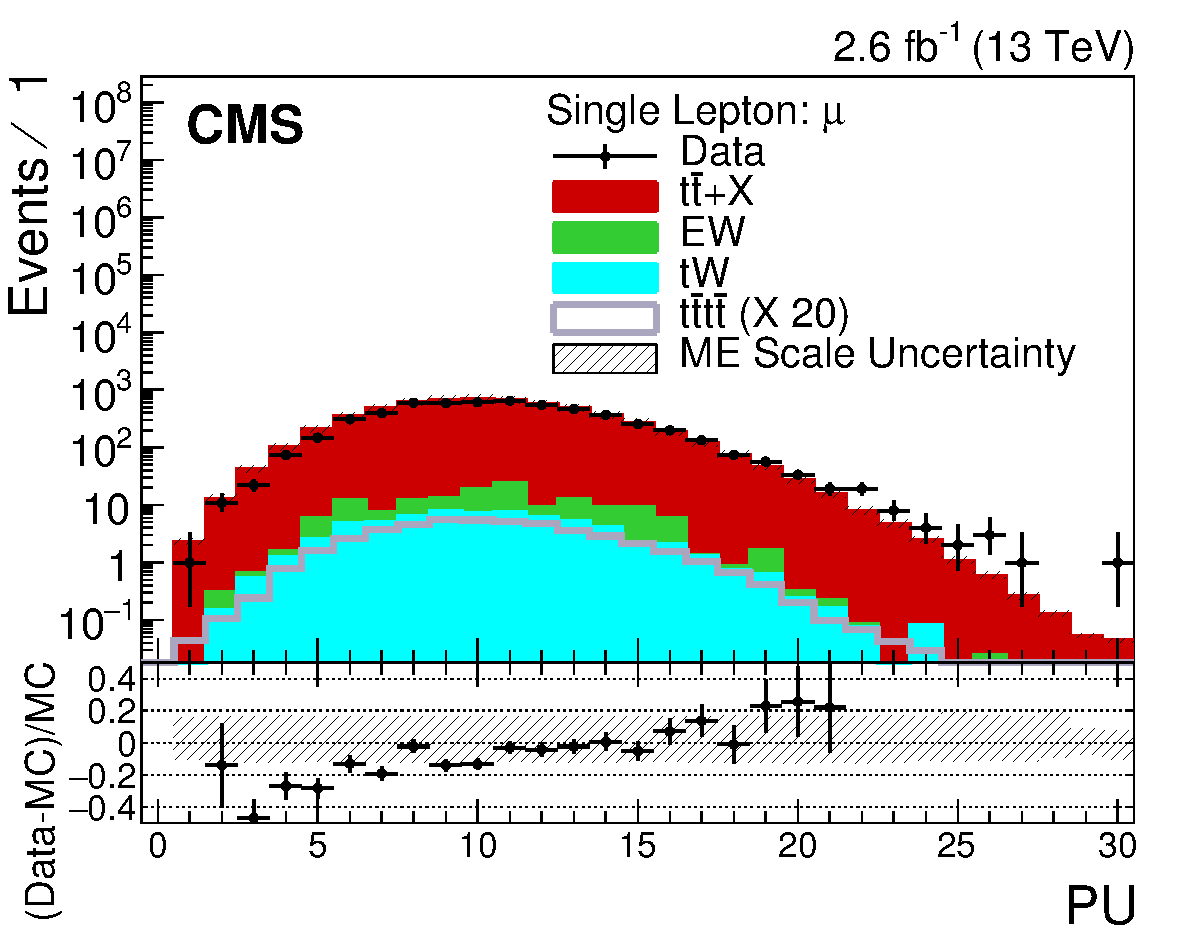
\includegraphics[width=0.67\textwidth]{images/Run2/PU_StackLogY.pdf}
\end{center}
\caption{The number of primary vertices for data and simulation after application of PU corrections for $\mu$ + jets.}
\label{fig:PUReWeight13}
\end{figure}

The method in Section~\ref{subsec:method2btag} was used to derive the b tagging scale factors. Figures~\ref{fig:csvJet3SF} and~\ref{fig:csvJet4SF} show the affect of applying the b-tagging scale factor to correct the CSV discriminator distributions and it can be seen that the agreement between data and simulation has been improved.

\begin{figure}[ht!]
    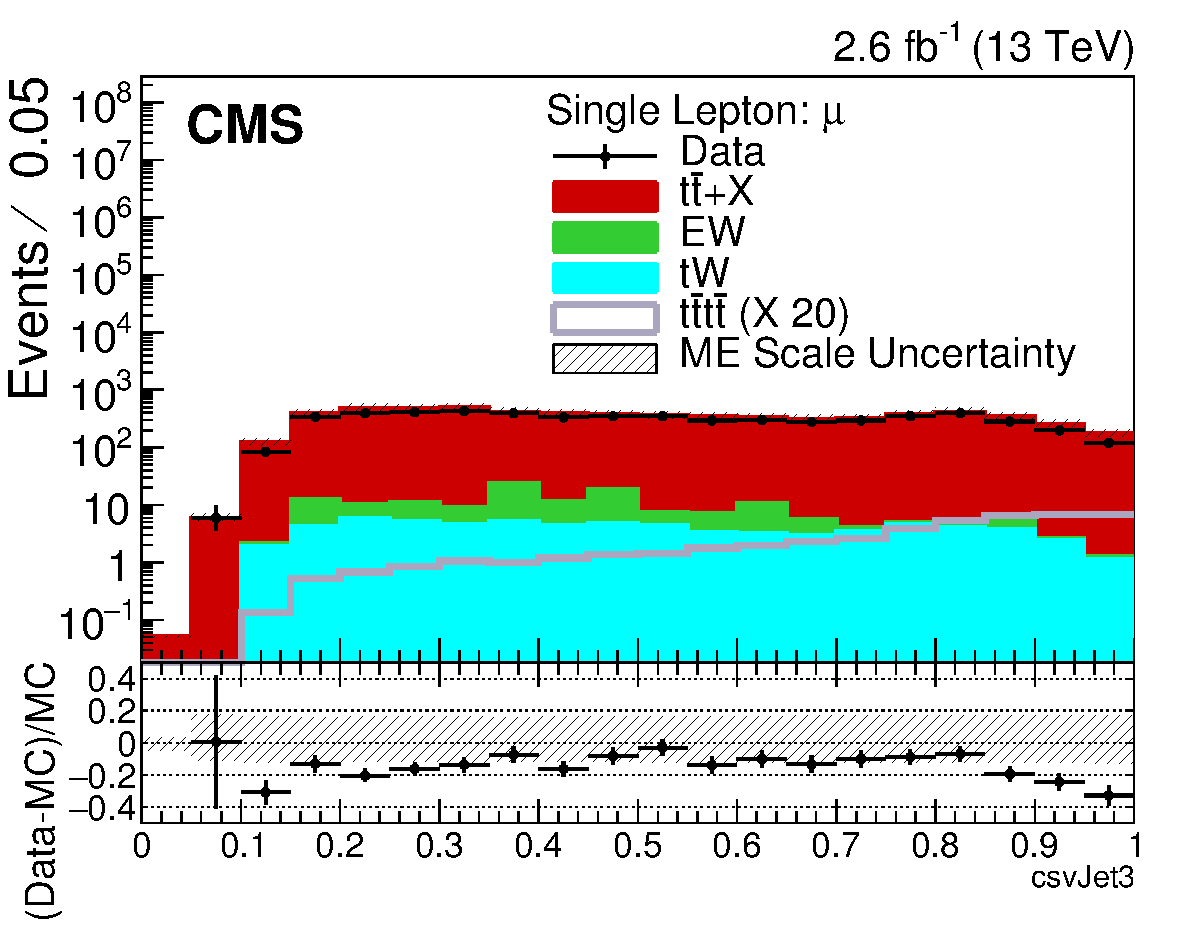
\includegraphics[width=0.48\textwidth]{images/Run2/csvJet3_StackLogY_noSF.pdf}
    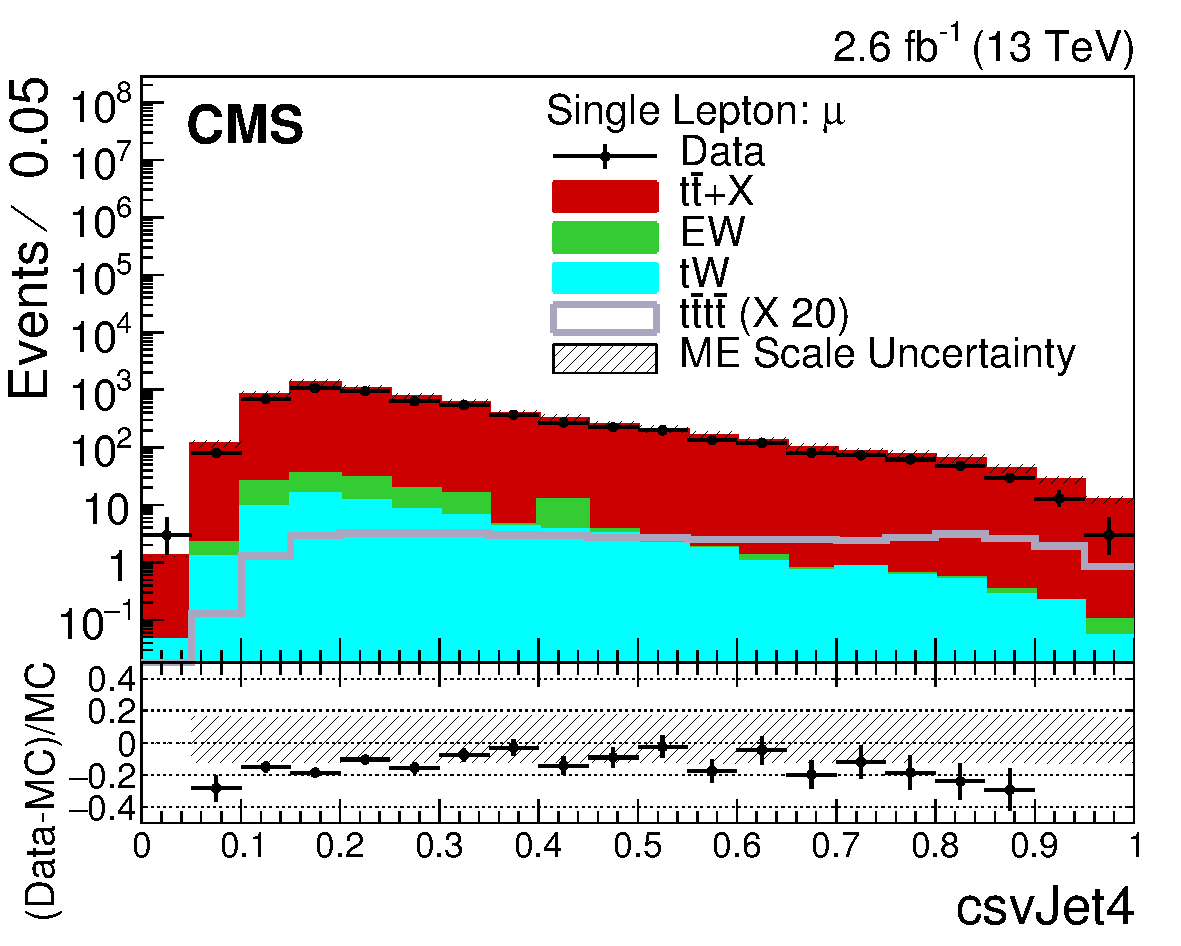
\includegraphics[width=0.48\textwidth]{images/Run2/csvJet4_StackLogY_noSF.pdf}
    \caption{ The third-highest and fourth-highest ranked CSV jet distributions for data and simulation in the $\mu$ + jets channel before b-tagging corrections, left and right respectively.}
    \label{fig:csvJet3SF}
\end{figure}
\begin{figure}[ht!]
    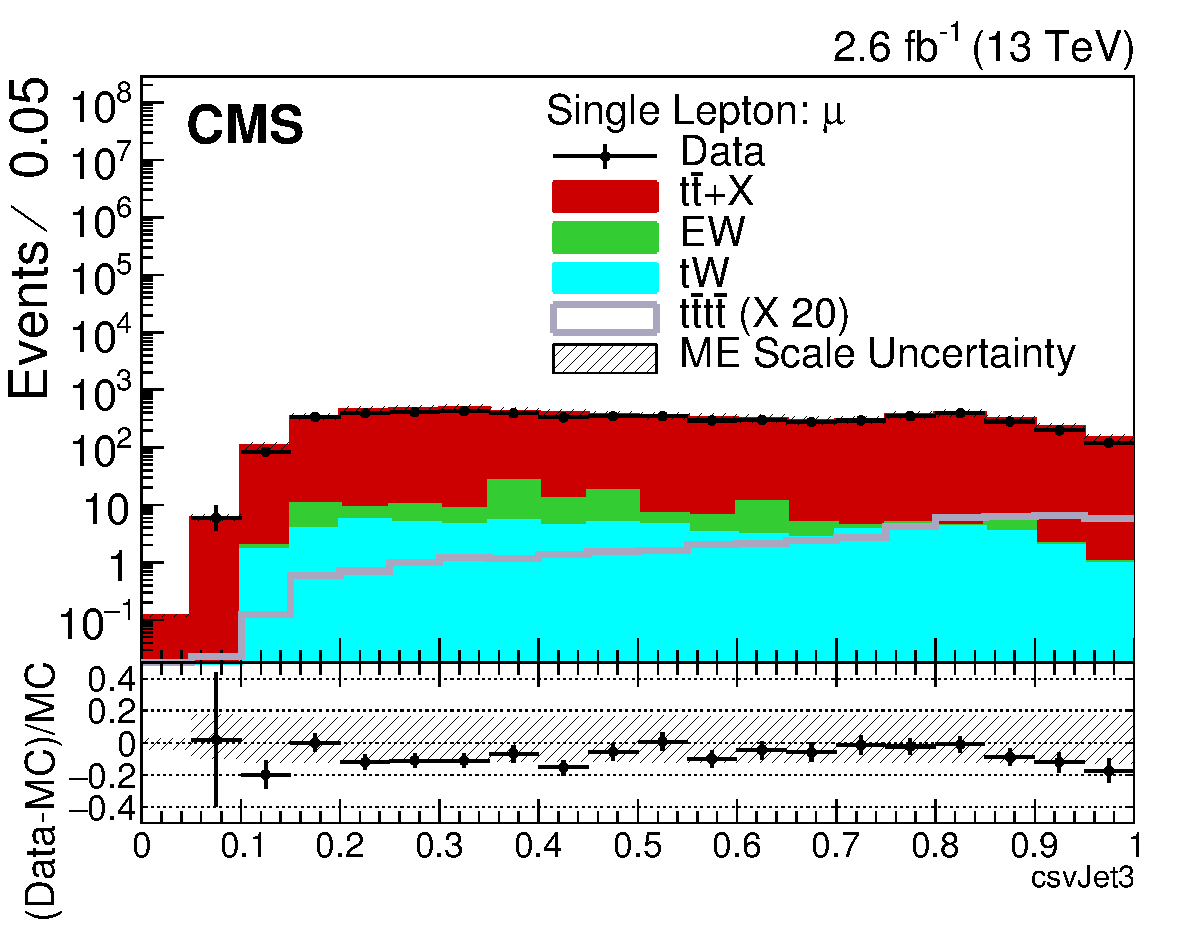
\includegraphics[width=0.48\textwidth]{images/Run2/csvJet3_StackLogY.pdf}
    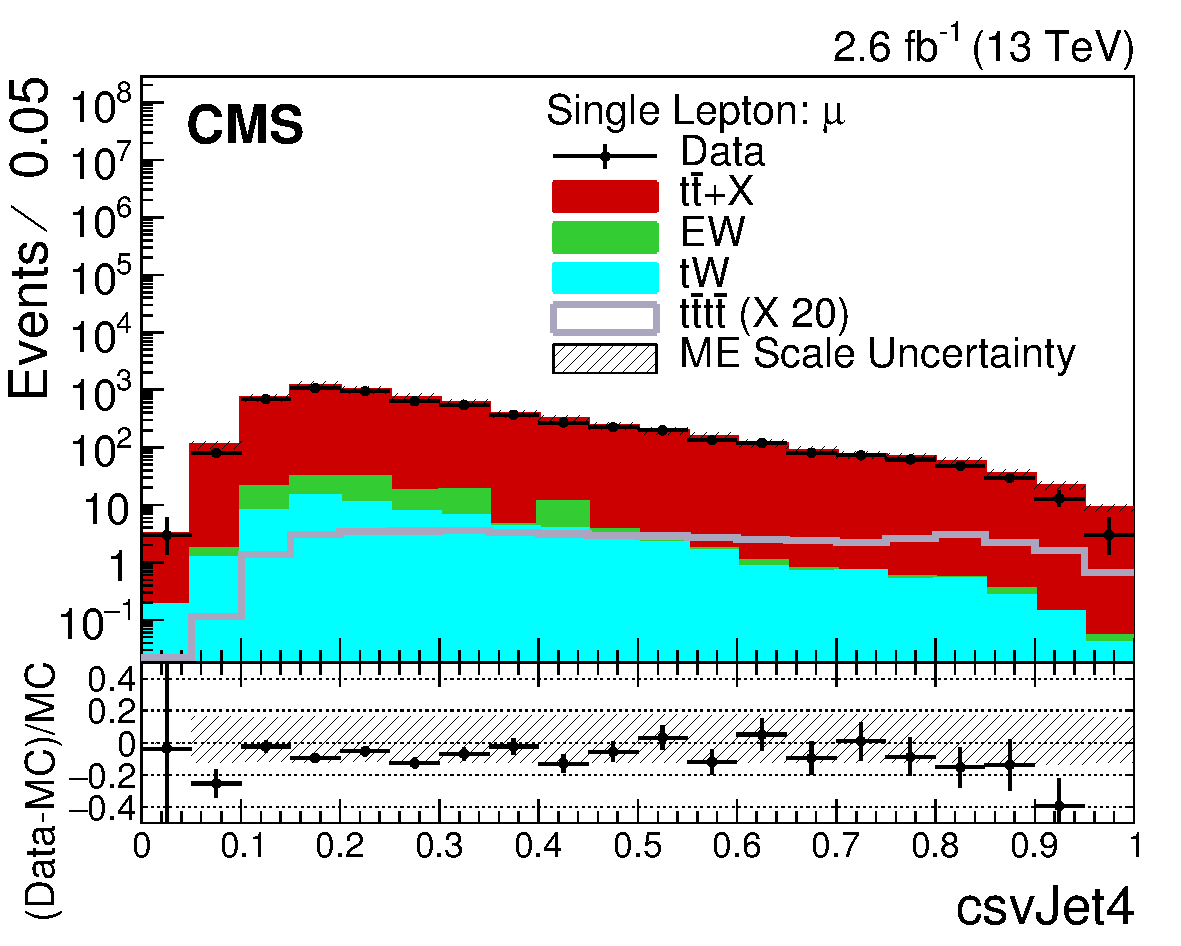
\includegraphics[width=0.48\textwidth]{images/Run2/csvJet4_StackLogY.pdf}
    \caption{The third-highest and fourth-highest ranked CSV jet distributions for data and simulation in the $\mu$ + jets channel after b-tagging corrections, left and right respectively.}
    \label{fig:csvJet4SF}
\end{figure}
 

The jet multiplicity modelling from Section~\ref{subsec:alphaS}, which corrects the MC to correspond to the best tune of $\alpha_S$ in simulation, was applied. It can be seen from Figs.~\ref{fig:withAlpha} and~\ref{fig:withoutAlpha} that the jet multiplicity modelling is greatly improved by applying this correction.

\begin{figure}[ht!]
    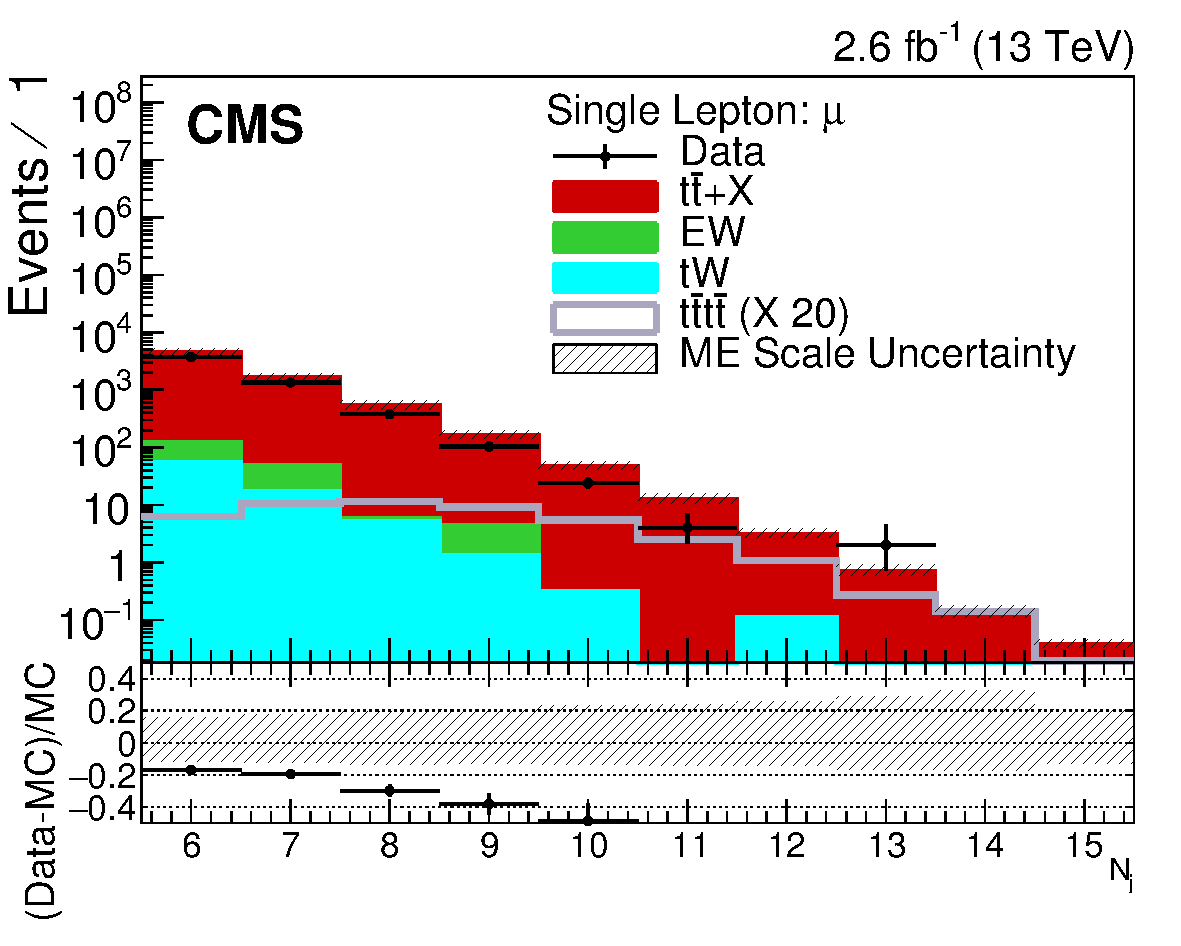
\includegraphics[width=0.48\textwidth]{images/Run2/nJets_StackLogY_woAlphaS.pdf}
    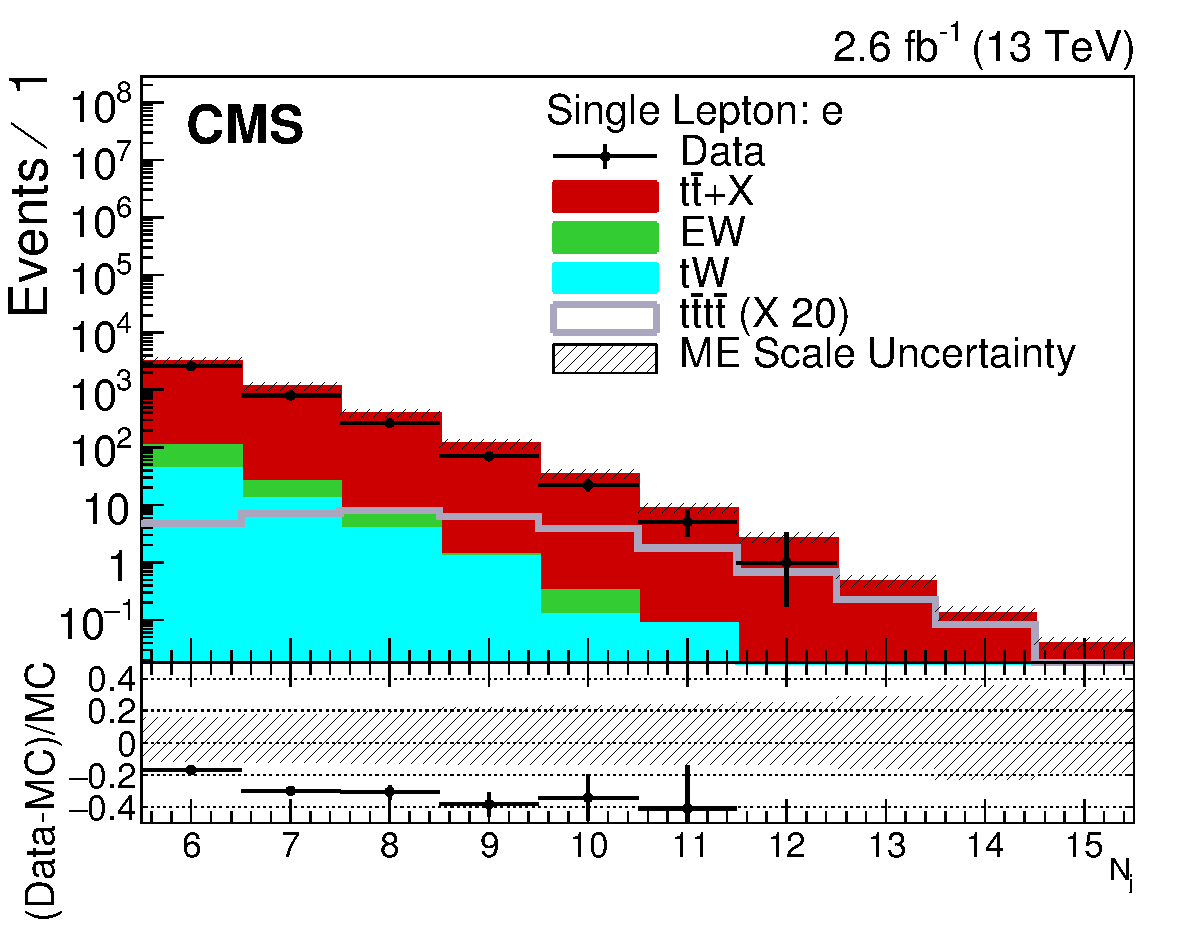
\includegraphics[width=0.48\textwidth]{images/Run2/nJets_StackLogY_e_woAlphaS.pdf}
    \caption{The \njets distributions for data and simulation in the $\mu$ + jets channel (left) and $e$ + jets channel (left) without jet multiplicity modelling scale factors applied.}
    \label{fig:withoutAlpha}
\end{figure}

\begin{figure}[ht!]
    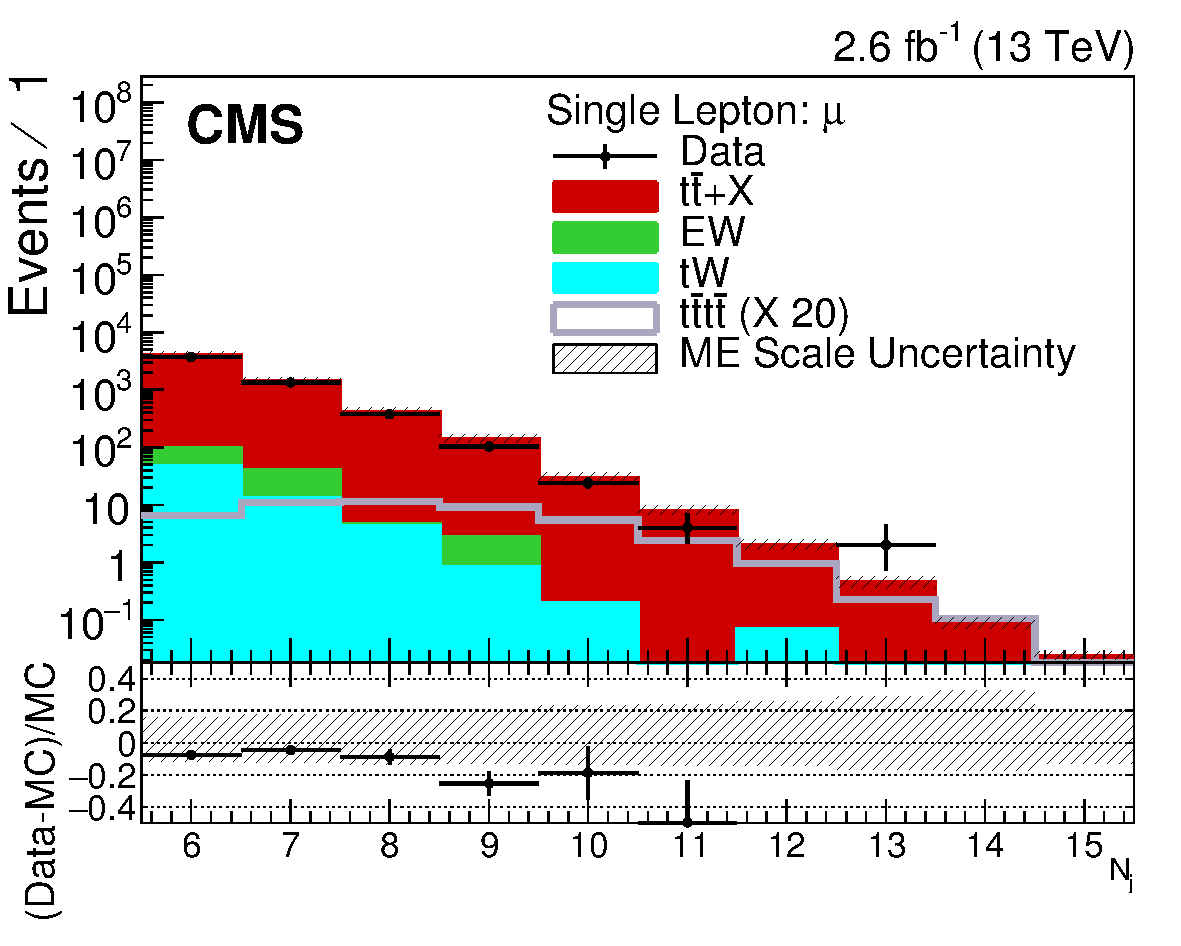
\includegraphics[width=0.48\textwidth]{images/Run2/nJets_StackLogY.pdf}
    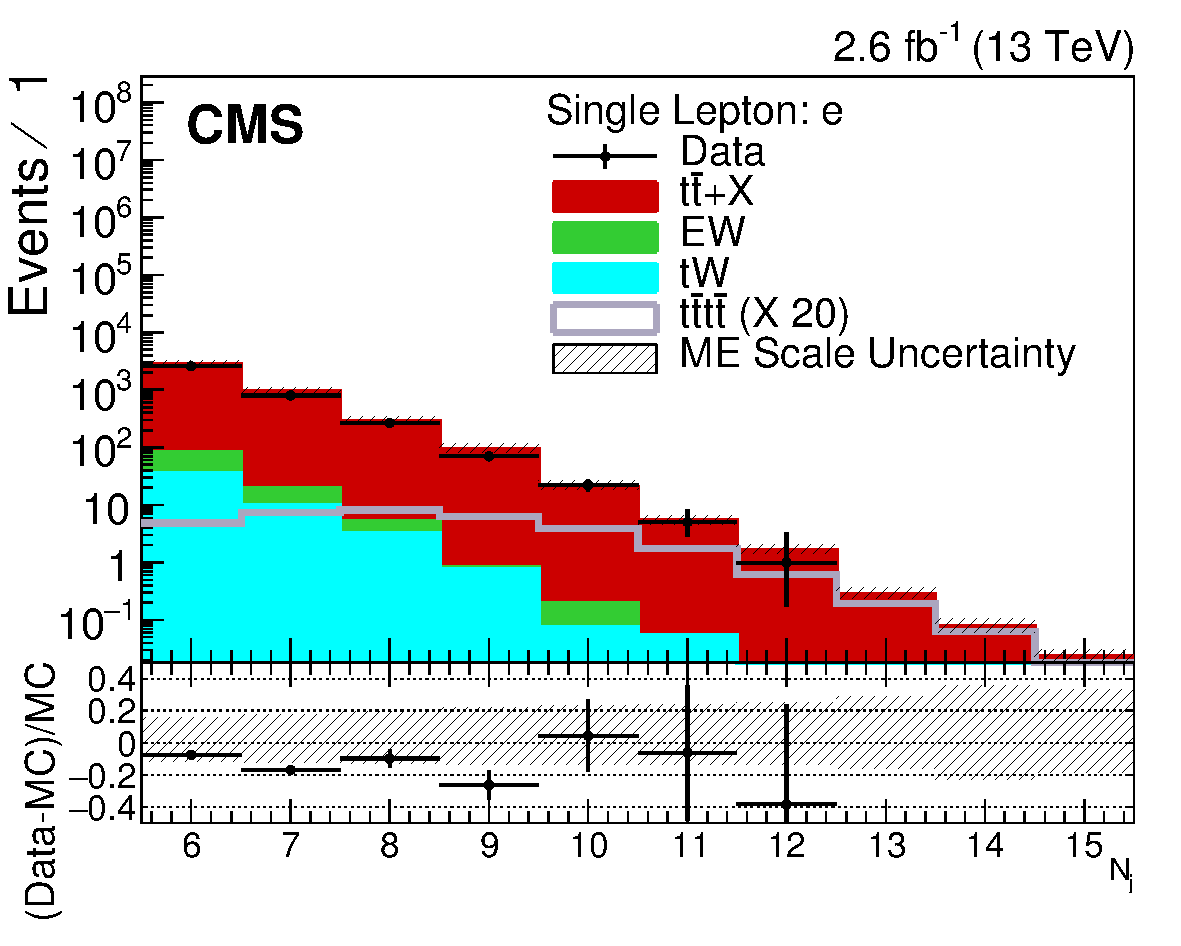
\includegraphics[width=0.48\textwidth]{images/Run2/nJets_StackLogY_e.pdf}
    \caption{The \njets distributions for data and simulation in the $\mu$ + jets channel (left) and $e$ + jets channel (left) with jet multiplicity modelling scale factors applied.}
    \label{fig:withAlpha}
\end{figure}


The scale factors applied for the heavy flavour modelling are described in Section~\ref{ttbbmod}. The distributions for the \nMtags are shown with and without the heavy flavour modelling scale factors applied. It is not obvious that there is a significant improvement in the \nMtags after the scale factors have been applied but the heavy flavour fraction is allowed to float as a shape nuisance parameter in the template fit.

\begin{figure}[ht!]
    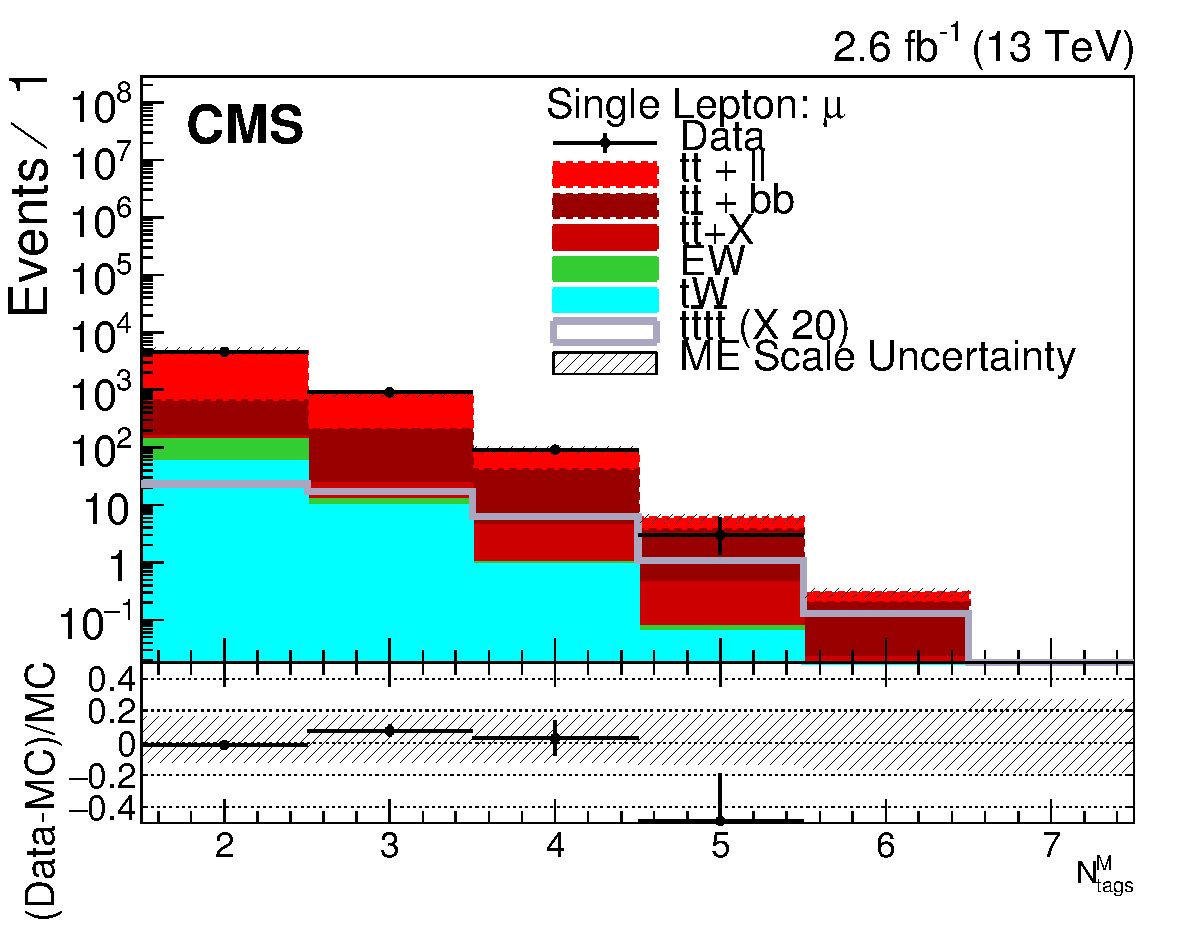
\includegraphics[width=0.47\textwidth]{images/Run2/nMtags_StackLogY_HF_wo_reweight.pdf} 
    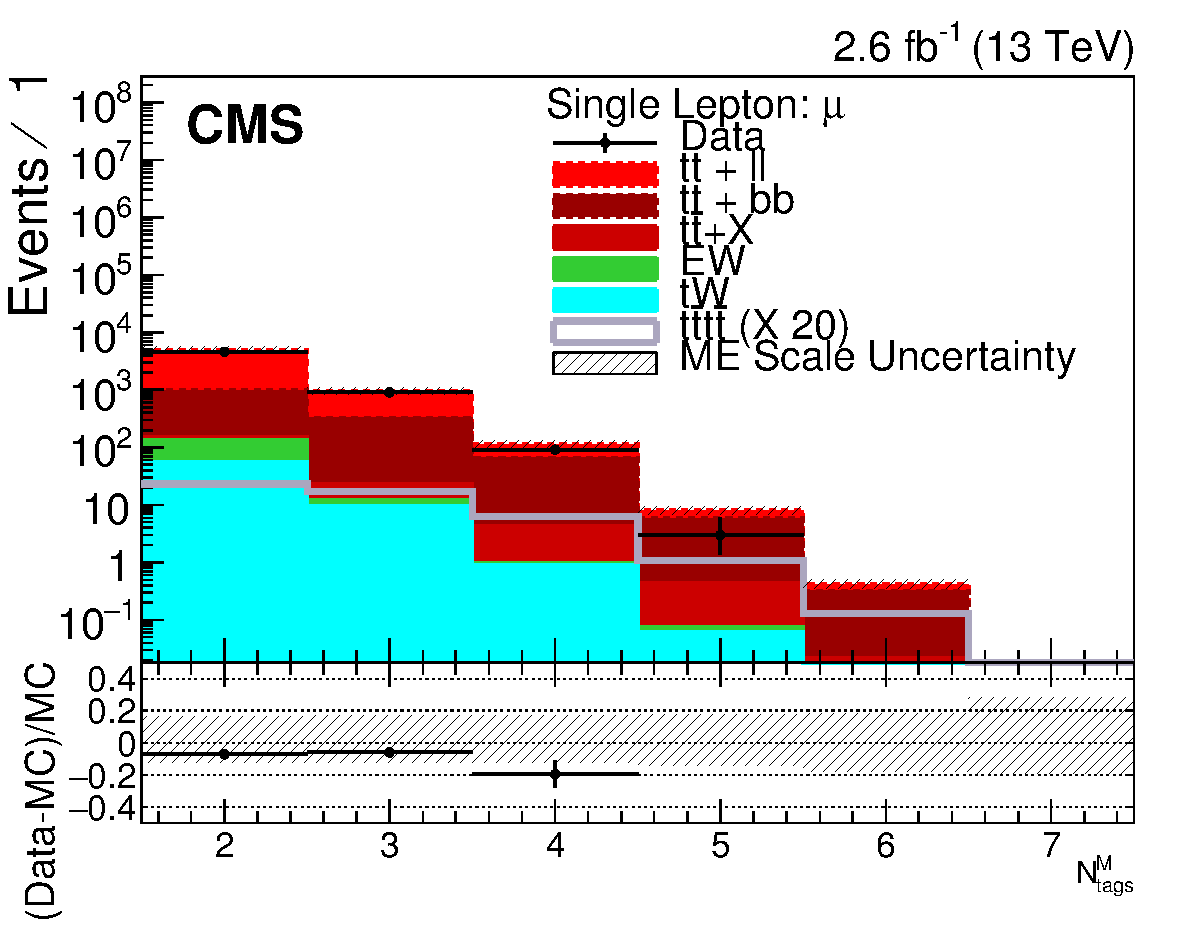
\includegraphics[width=0.47\textwidth]{images/Run2/nMtags_StackLogY_HF_w_reweight.pdf} 
    \caption{\nMtags are shown for the muon channel with heavy flavour reweighting (right) and without(left).}
    \label{fig:HF_reweight}
\end{figure}

\clearpage

\section{Effect of selection requirements \label{cutflow13}}

The event counts, weighted by each correction factor in MC, are given after each selection requirement for $\mu$ + jets in Table~\ref{tab:museltable} and e + jets in Table~\ref{tab:eseltable}.
% In tables~\ref{tab:museltable} and~\ref{tab:eseltable}, the numbers of data events selected and the weighted number of simulated events expected after each step of the $\mu$ + jets and e + jets baseline selections are detailed respectively. 
Small discrepancies between the initial simulated events in each table are due to different lepton scale factors being applied in each case.
After the baseline selection has been applied the \ttbar component represents $\approx 97\%$ of the background samples combined. The ttbb and ttll/ttcc components of the main \ttbar sample are also given in the tables. \ttZ and \ttW have been merged into TTV for the tables.
Note that these studies were performed when method 1 from Section~\ref{subsec:method1btag} was used for b-tagging before the analysis was updated to using method 2 from Section~\ref{subsec:method2btag}.

\begin{table}[ht!]
\small
\caption{Number of events after successive selection requirements in the $\mu$ + jets channel ($\mathcal{L}=2.6~\fb$)}
\label{tab:museltable}
\centering
\begin{tabular}{c|cccccccc|cc}

\hline

& \tiny Data & \tiny  \tttt     & \tiny Single top      & \tiny DY   & \tiny W   & \tiny \ttH   & \tiny TTV  & \tiny \ttbar & \tiny ttbb & \tiny ttll\&ttcc \\

\hline
\tiny initial&       \tiny 85493692     & \tiny 24.83  & \tiny 90650       & \tiny 16047092   & \tiny 164877974  & \tiny 751.39 & \tiny 1310 & \tiny 2129712 &      \tiny    104490.21       & \tiny 2025221.86     \\

\tiny Is Good PV&    \tiny 85162369     & \tiny 24.82  & \tiny 90614       & \tiny 15965470   & \tiny 164144695  & \tiny 751.11 & \tiny 1309.5 & \tiny 2128929 &    \tiny   104462.79       & \tiny 2024466.92   \\

\tiny Trigger&        \tiny55410616     & \tiny 6.66   & \tiny 14609       & \tiny 3878887    & \tiny 27271551   & \tiny 112.68 & \tiny 371 & \tiny 327184 &       \tiny   15017.71        & \tiny 312166.40     \\

\tiny Exactly 1 mu&  \tiny 21066450     & \tiny 4.57   & \tiny 11204       & \tiny 1573769    & \tiny 18270602   & \tiny 82.65  & \tiny 248 & \tiny 243848  &  \tiny   11164.52        & \tiny 232684.31    \\

\tiny lepton Veto&   \tiny 20175902     & \tiny 3.16   & \tiny 9715        & \tiny 889705.6     & \tiny 18258830   & \tiny 72.03  & \tiny 161.9  & \tiny 211962  &   \tiny   9861.60 & \tiny 202101.02       \\

\tiny $\geq$ 1 Jets&       \tiny 4620960      & \tiny 3.16   & \tiny 9442.02        & \tiny 265849.57      & \tiny 3055360.09     & \tiny 72   & \tiny 161.3  & \tiny 210197 &      \tiny    9839.65 & \tiny 200357.37    \\

\tiny $\geq$ 6 Jets&        \tiny13642        & \tiny 2.84   & \tiny 171.23 & \tiny 195.01 & \tiny 1533.65        & \tiny 24.78  & \tiny 29.9  & \tiny 11621   &        \tiny  1319.14 & \tiny 10302.68      \\

\tiny $\geq$ 2 CSVM bs&  \tiny 5134 & \tiny 2.14   & \tiny 62.73  & \tiny 10.40  & \tiny 63.76  & \tiny 20.02  & \tiny 12.6   & \tiny 5169    &  \tiny   656.85  & \tiny 4512.54    \\


\hline
\end{tabular}
\end{table}

%\begin{landscape}
\begin{table}[ht!]
\small
\caption{Number of events after successive selection requirements in the e + jets channel ($\mathcal{L}=2.6~\fb$)} %(2.6 \fbinv of int. lumi.)}
\label{tab:eseltable}
\centering
\begin{tabular}{c|cccccccc|cc}
\hline
& \tiny Data & \tiny  \tttt     & \tiny Single top      & \tiny DY   & \tiny W   & \tiny \ttH   & \tiny TTV  & \tiny \ttbar & \tiny ttbb & \tiny ttll\&ttcc \\

\hline
\tiny initial& \tiny         124817372    & \tiny 24.85  & \tiny 90654.24       & \tiny 16064098    & \tiny 165066697   & \tiny 751.61 & \tiny 1311 & \tiny 2130186  &    \tiny    104478.04       & \tiny 2025708.35   \\

\tiny Is Good PV& \tiny      124485606    & \tiny 24.85  & \tiny 90617.89       & \tiny 15982367    & \tiny 164331394   & \tiny 751.32 & \tiny 1310  & \tiny 2129403 &   \tiny  104450.58       & \tiny 2024952.90      \\

\tiny Trigger& \tiny         110109139    & \tiny 5.72   & \tiny 12032.47       & \tiny 3197556     & \tiny 20048189    & \tiny 93.63  & \tiny 327.3 & \tiny 265851  &   \tiny     12262.32        & \tiny 253589.27      \\

\tiny Exactly 1 e& \tiny     13274896     & \tiny 3.45   & \tiny 8047.12        & \tiny 1413711     & \tiny 10109490    & \tiny 59.11  & \tiny 196.3 & \tiny 170369  &  \tiny  7805.28 & \tiny 162564.24      \\

\tiny lepton Veto& \tiny     12501476     & \tiny 2.24   & \tiny 6809.00        & \tiny 692211      & \tiny 10102672    & \tiny 50.38  & \tiny 117.6  & \tiny 144686  & \tiny   6751.00 & \tiny 137935.73       \\

\tiny $\geq$ 1 Jets& \tiny         3802752      & \tiny 2.24   & \tiny 6620.41        & \tiny 374277      & \tiny 1927106     & \tiny 111.3  & \tiny 56.25  & \tiny 143511  &   \tiny     6736.26 & \tiny 136775.28     \\

\tiny $\geq$ 6 Jets& \tiny         9930 & \tiny 2.01   & \tiny 128.79 & \tiny 214.01 & \tiny 1071.71        & \tiny 17.54  & \tiny 22.6   & \tiny 8086.18   &      \tiny  922.58  & \tiny 7163.61       \\

\tiny $\geq$ 2 CSVM bs& \tiny    3577 & \tiny 1.51   & \tiny 48.82  & \tiny 12.54  & \tiny 42.87  & \tiny 14.16  & \tiny 9.4  & \tiny 3592.65    & \tiny  461.90  & \tiny 3130.74          \\

\hline
\end{tabular}
\end{table}

\section{Control distributions between data and simulation}
Distributions are shown for HTb, \HTrat, $p_{\textrm{T trijet1}}$, \nLtags, \nTtags, \redhadmass, \HTX and lepton isolation. Good agreement is seen between data and simulation in all distributions with almost all data points within the ME scale uncertainty, the dominant systematic uncertainty, represented by the hatched band.

\begin{figure}[ht!]
    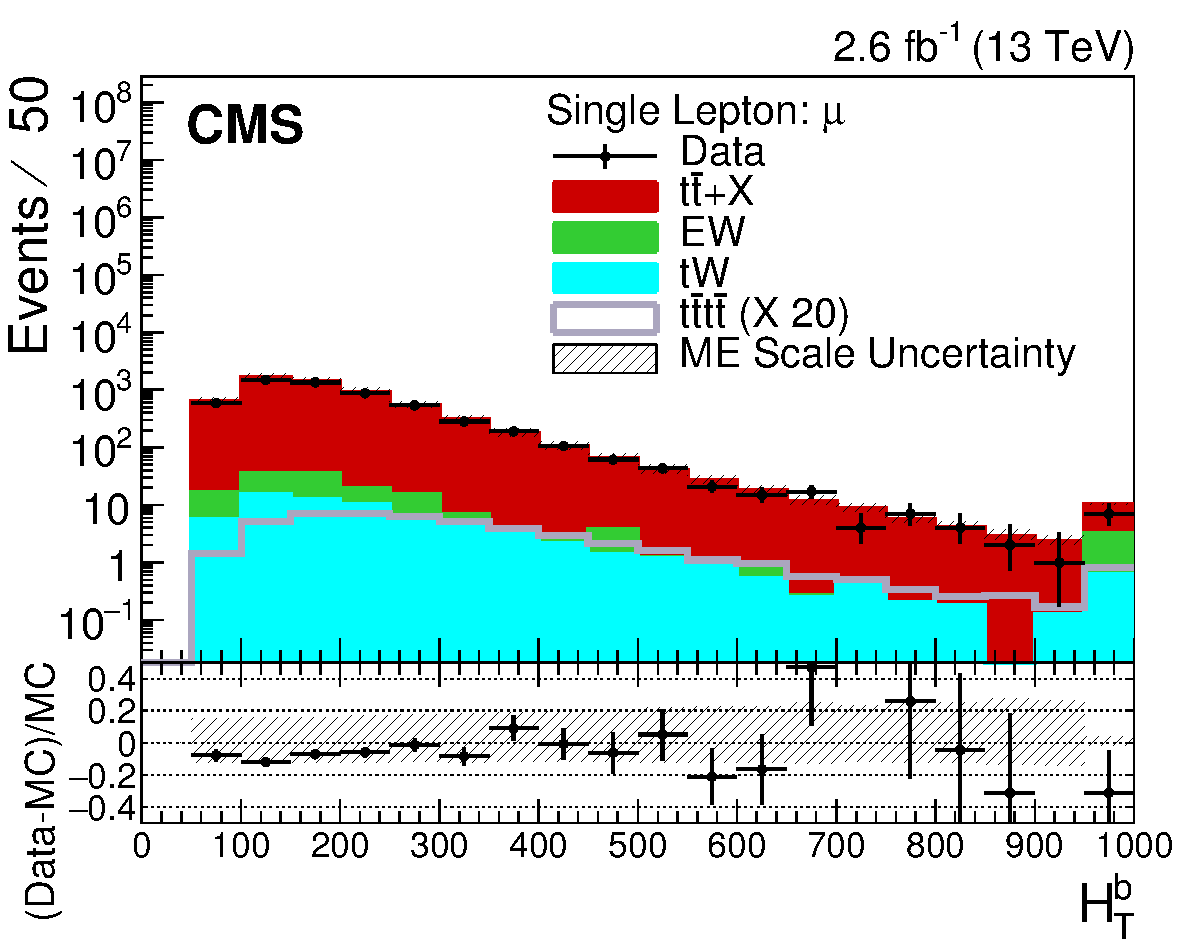
\includegraphics[width=0.48\textwidth]{images/Run2/HTb_StackLogY.pdf}
    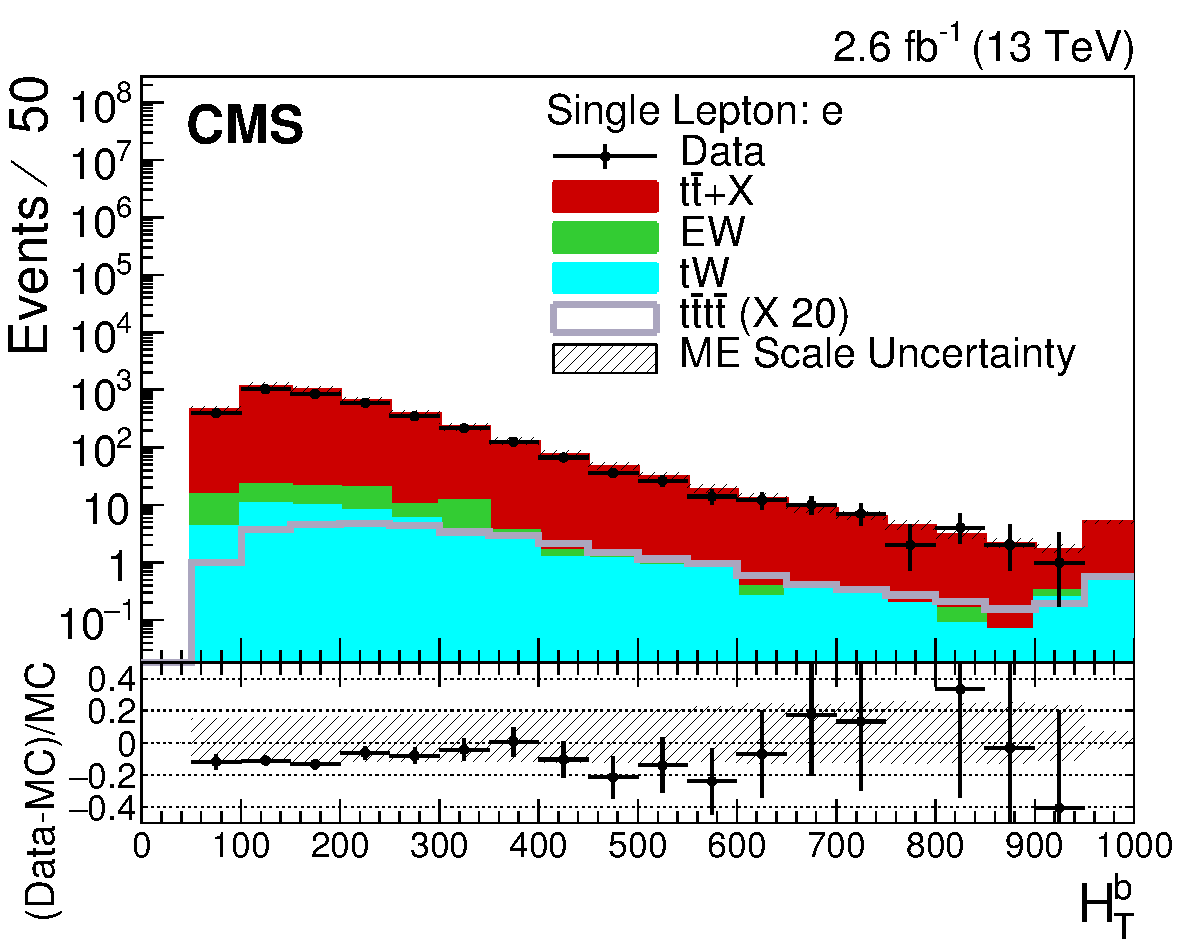
\includegraphics[width=0.48\textwidth]{images/Run2/HTb_StackLogY_e.pdf}
    \caption{The HTb distributions for data and simulation in the $\mu$ + jets channel (left) and $e$ + jets channel (left).}
    \label{fig:HTB}
\end{figure}


\begin{figure}[ht!]
    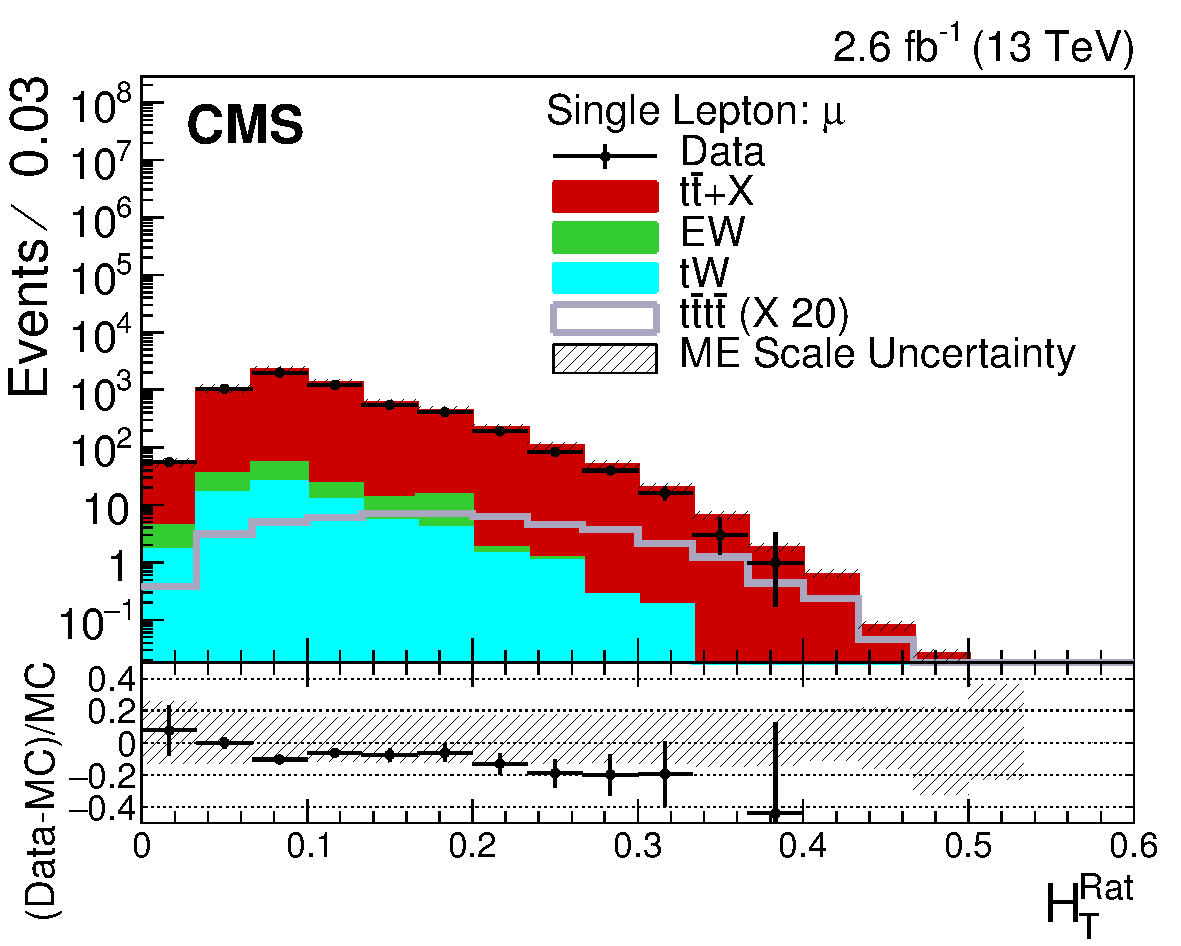
\includegraphics[width=0.48\textwidth]{images/Run2/HTRat_StackLogY.pdf}
    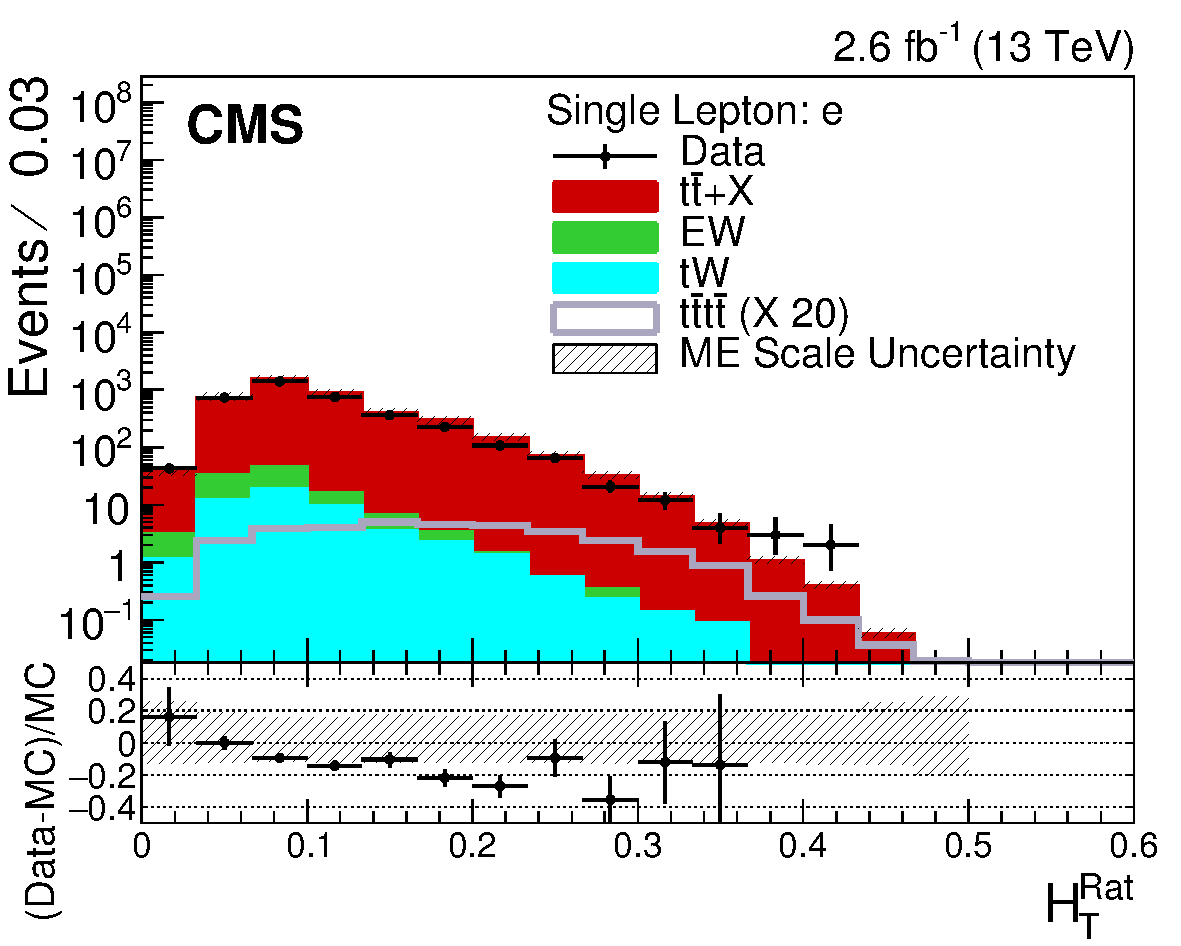
\includegraphics[width=0.48\textwidth]{images/Run2/HTRat_StackLogY_e.pdf}
    \caption{The \HTrat distributions for data and simulation in the $\mu$ + jets channel (left) and $e$ + jets channel (left).}
    \label{fig:HTRat}
\end{figure}



% \begin{figure}[ht!]
%     \includegraphics[width=0.48\textwidth]{images/Run2/LeadingBJetPt_StackLogY.pdf}
%     \includegraphics[width=0.48\textwidth]{images/Run2/LeadingBJetPt_StackLogY.pdf}
%     \caption{The \leadbpt distributions for data and simulation in the $\mu$ + jets channel (left) and $e$ + jets channel (left).}
%     \label{fig:LeadingBJetPt}
% \end{figure}

    
\begin{figure}[ht!]
    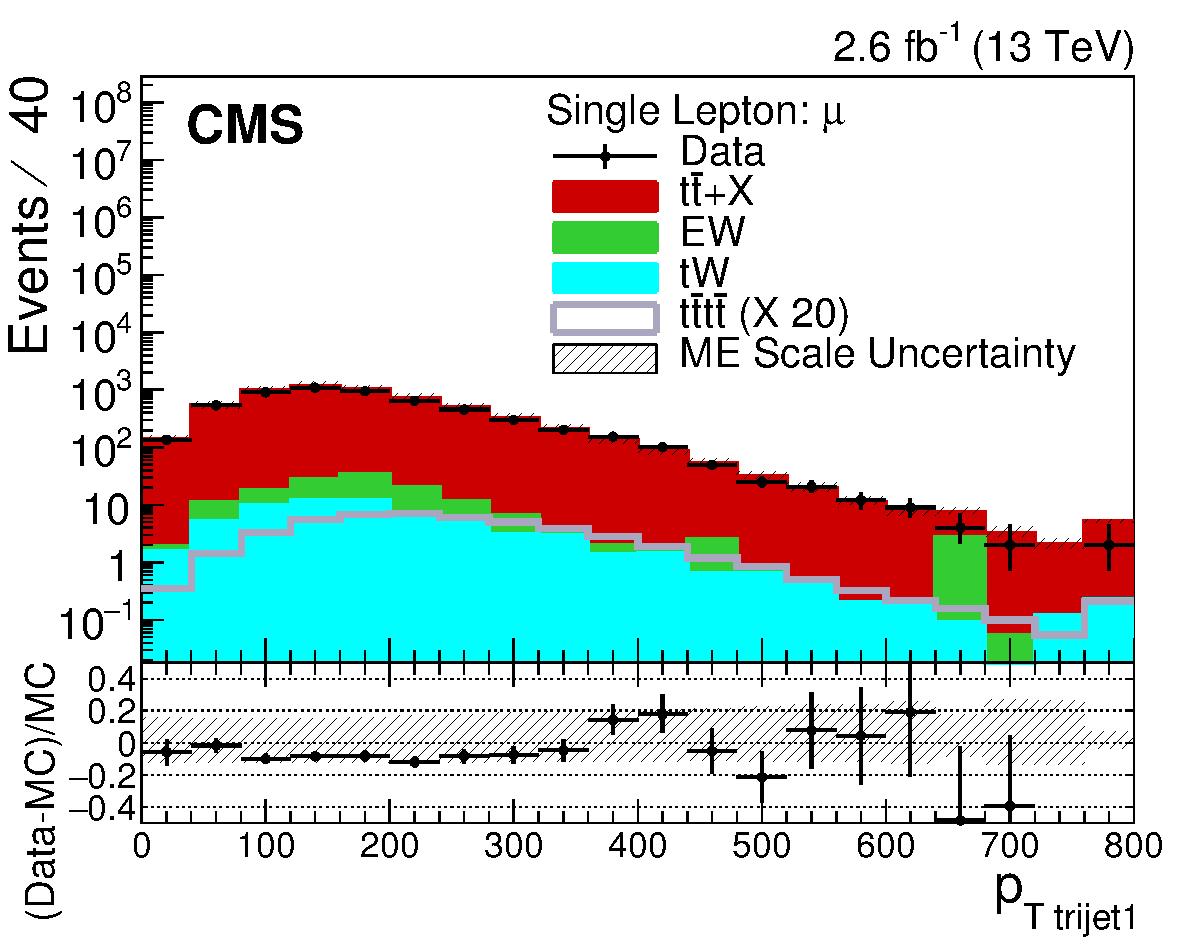
\includegraphics[width=0.48\textwidth]{images/Run2/bestTopPt_StackLogY.pdf}
    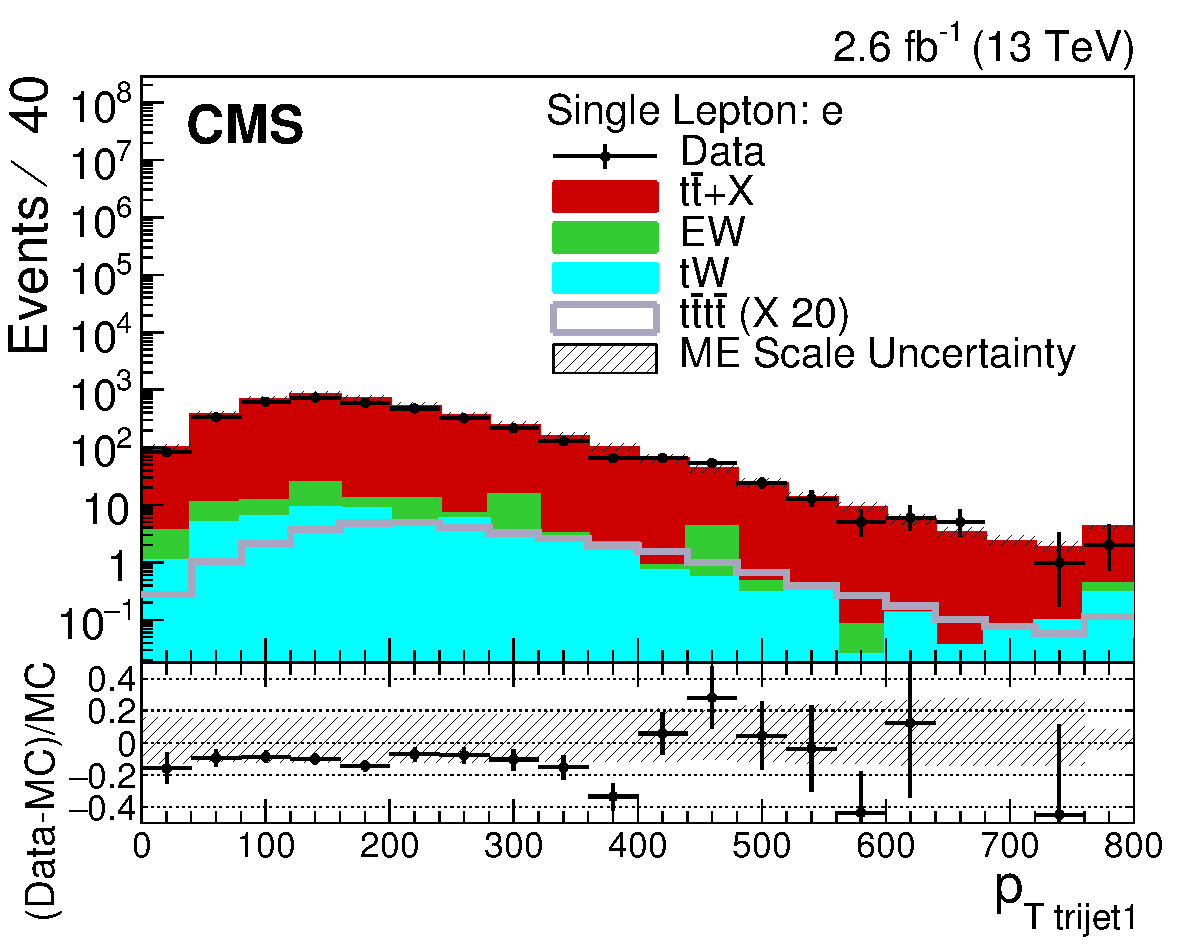
\includegraphics[width=0.48\textwidth]{images/Run2/bestTopPt_StackLogY_e.pdf}
    \caption{The $p_{\textrm{T trijet1}}$ distributions for data and simulation in the $\mu$ + jets channel (left) and $e$ + jets channel (left).}
    \label{fig:bestTopPt}
\end{figure}
   

\begin{figure}[ht!]
    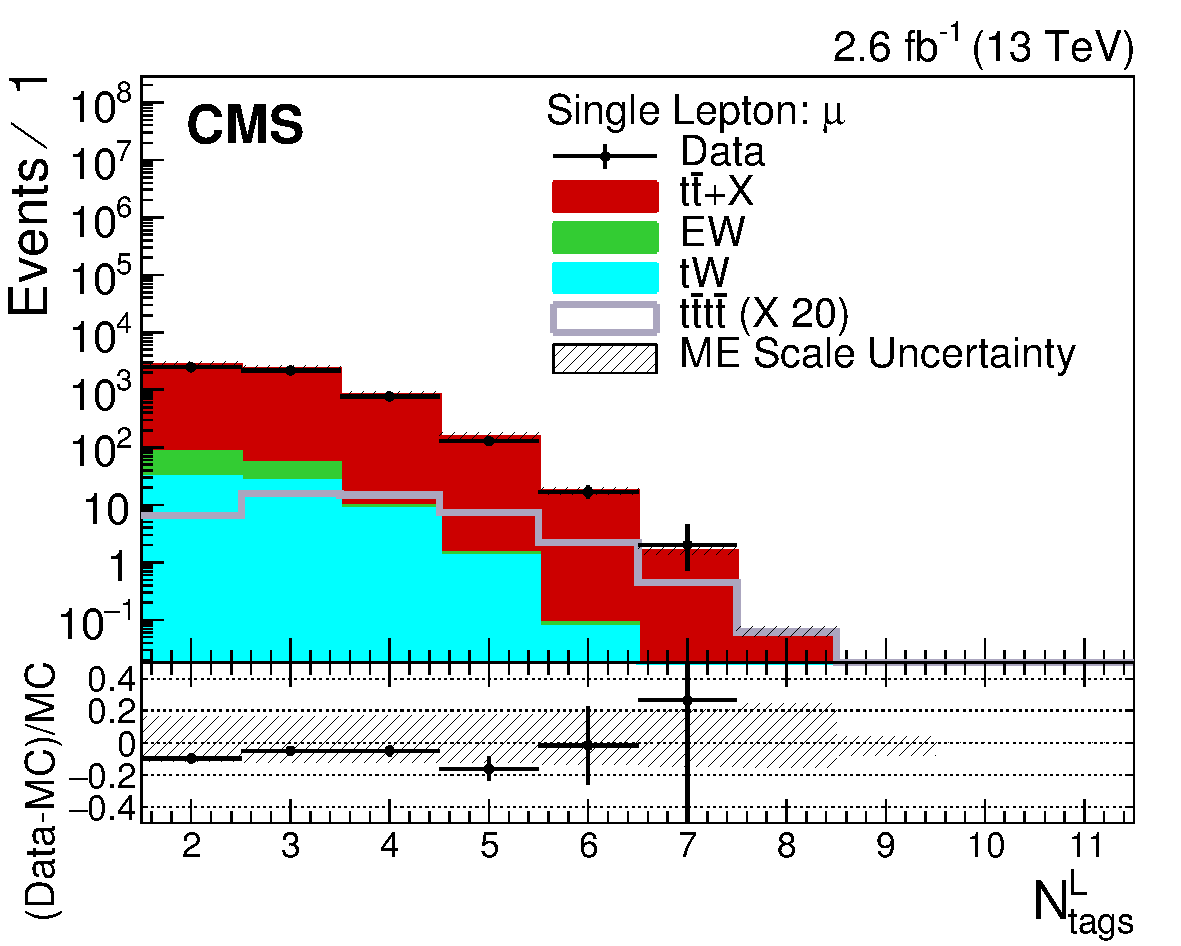
\includegraphics[width=0.48\textwidth]{images/Run2/nLtags_StackLogY.pdf}
    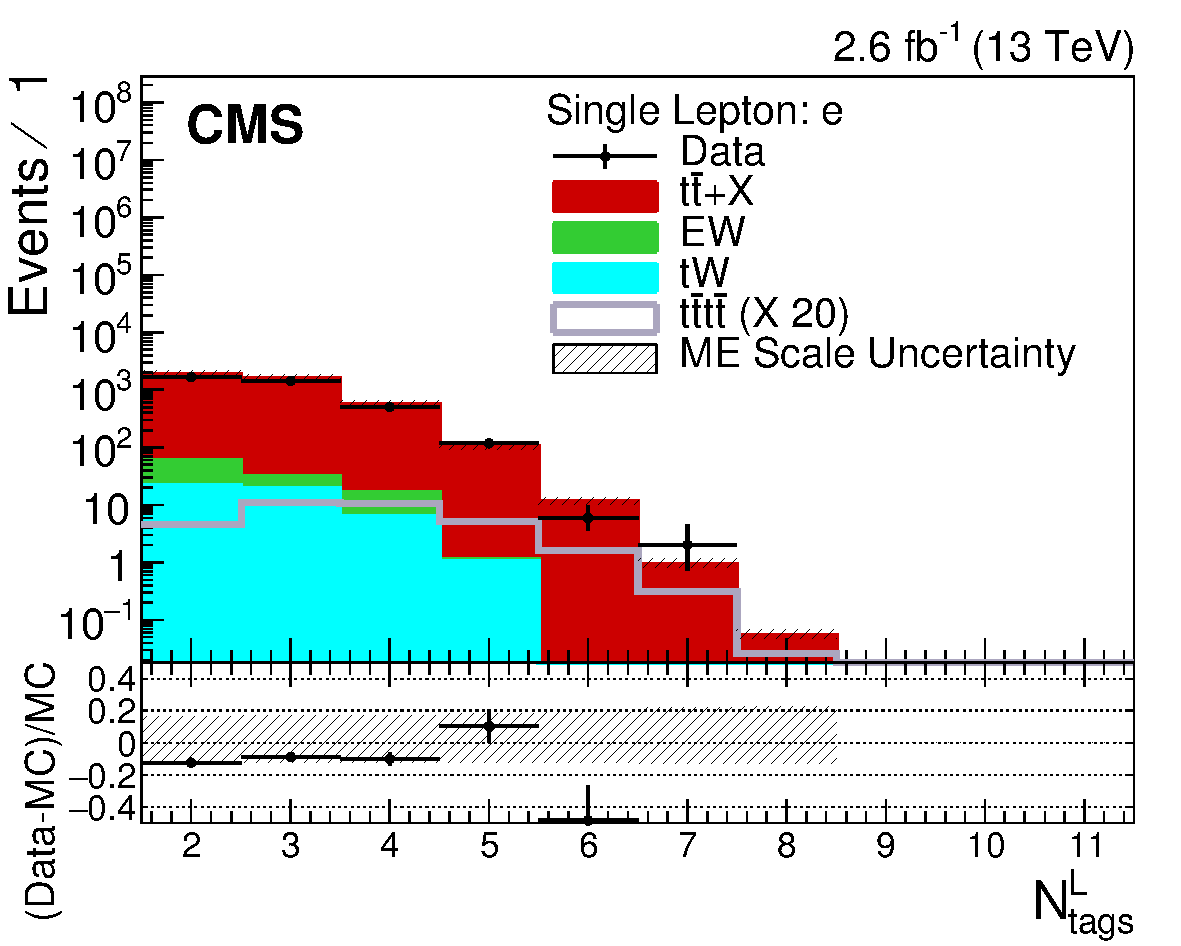
\includegraphics[width=0.48\textwidth]{images/Run2/nLtags_StackLogY_e.pdf}
    \caption{The \nLtags distributions for data and simulation in the $\mu$ + jets channel (left) and $e$ + jets channel (left).}
    \label{fig:nLtagsInc}
\end{figure}

\begin{figure}[ht!]
    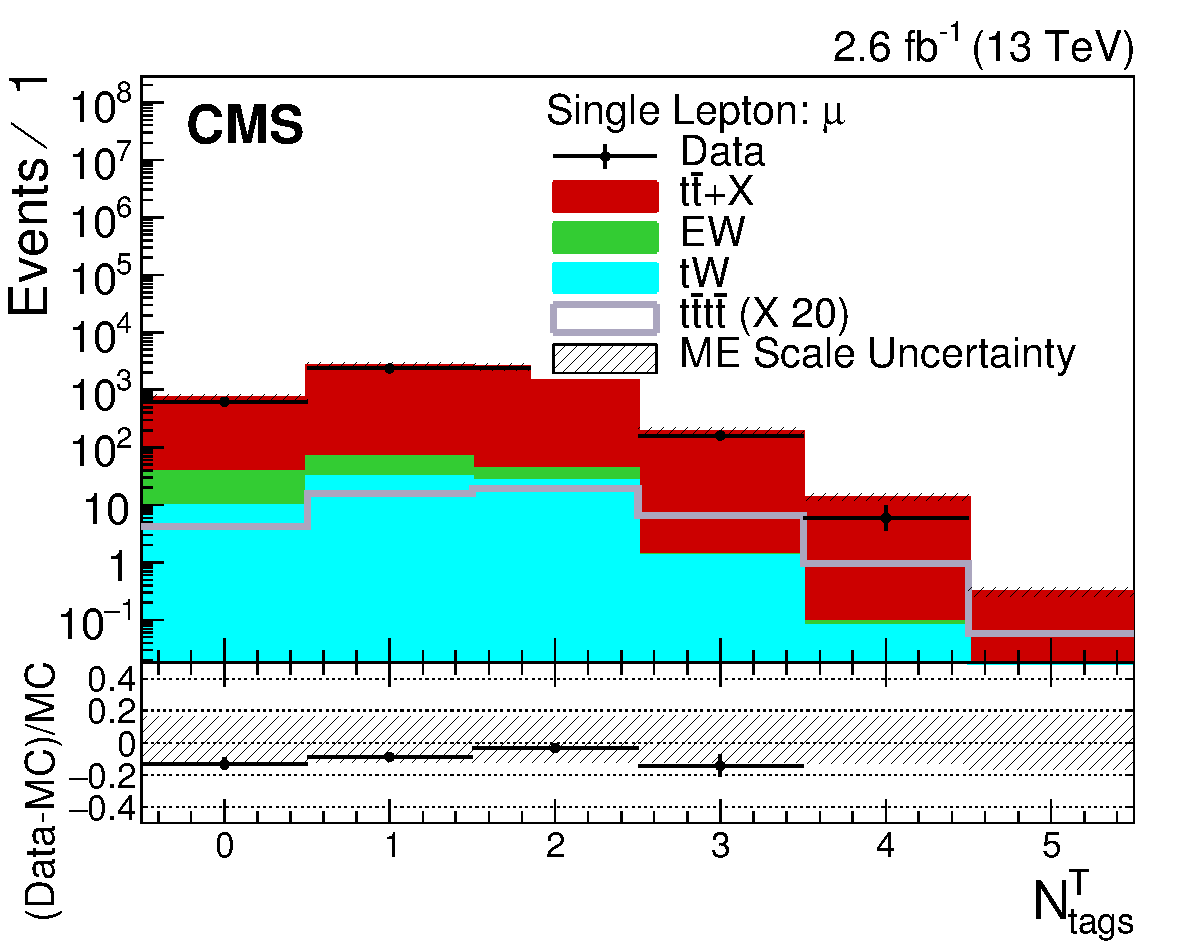
\includegraphics[width=0.48\textwidth]{images/Run2/nTtags_StackLogY.pdf}
    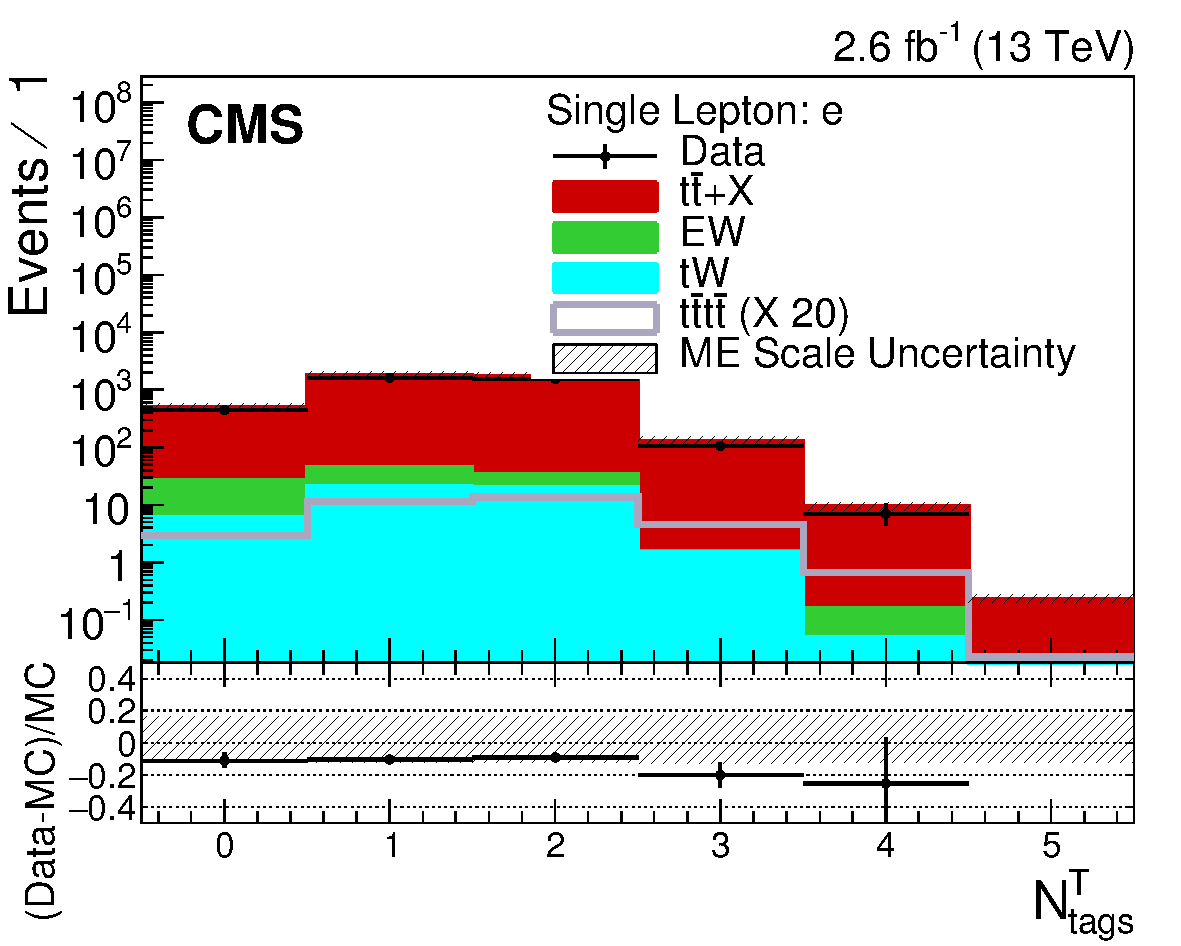
\includegraphics[width=0.48\textwidth]{images/Run2/nTtags_StackLogY_e.pdf}
    \caption{The \nTtags distributions for data and simulation in the $\mu$ + jets channel (left) and $e$ + jets channel (left).}
    \label{fig:nTtagsInc}
\end{figure}

\begin{figure}[ht!]
    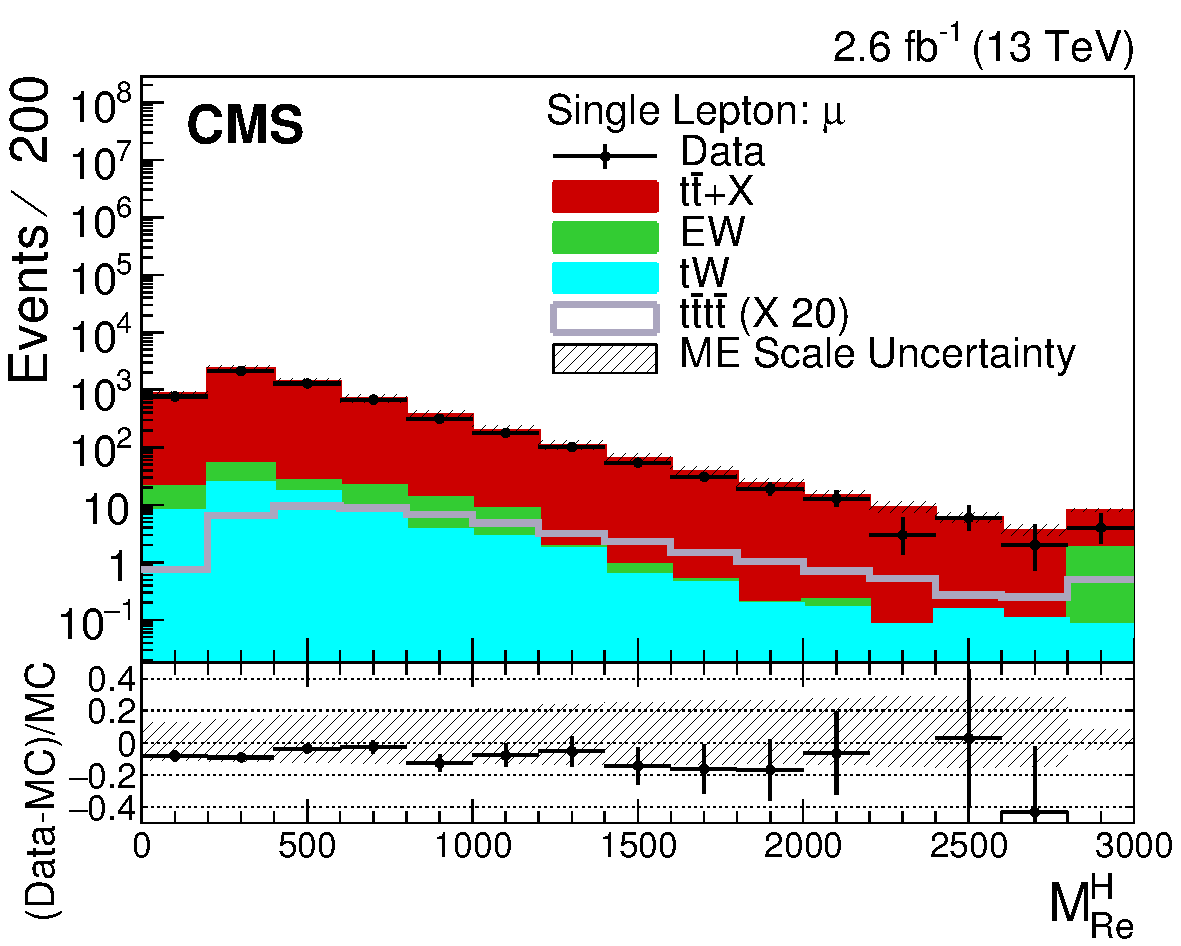
\includegraphics[width=0.48\textwidth]{images/Run2/SumJetMassX_StackLogY.pdf}
    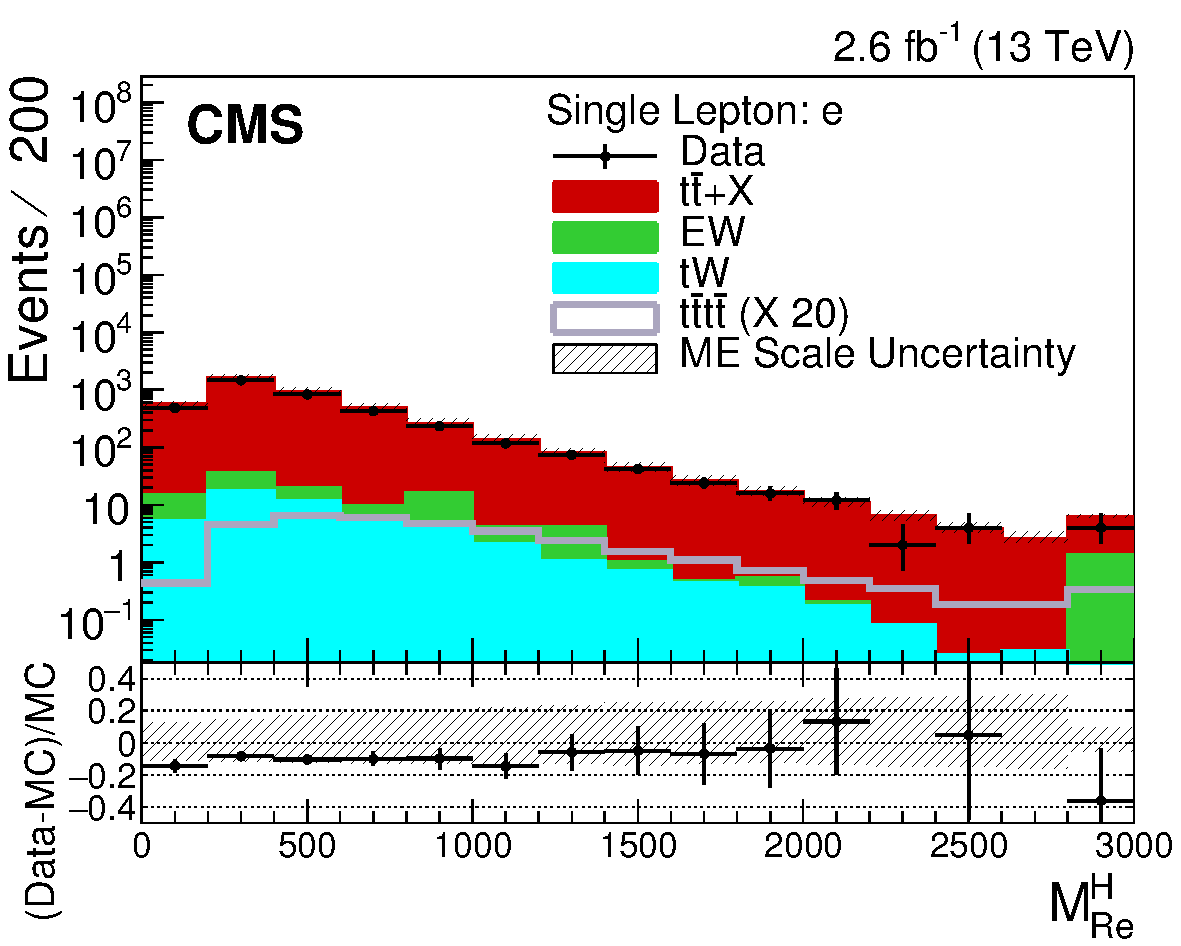
\includegraphics[width=0.48\textwidth]{images/Run2/SumJetMassX_StackLogY_e.pdf}
    \caption{The \redhadmass distributions for data and simulation in the $\mu$ + jets channel (left) and $e$ + jets channel (left).}
    \label{fig:SumJetMassX}
\end{figure}

\begin{figure}[ht!]
    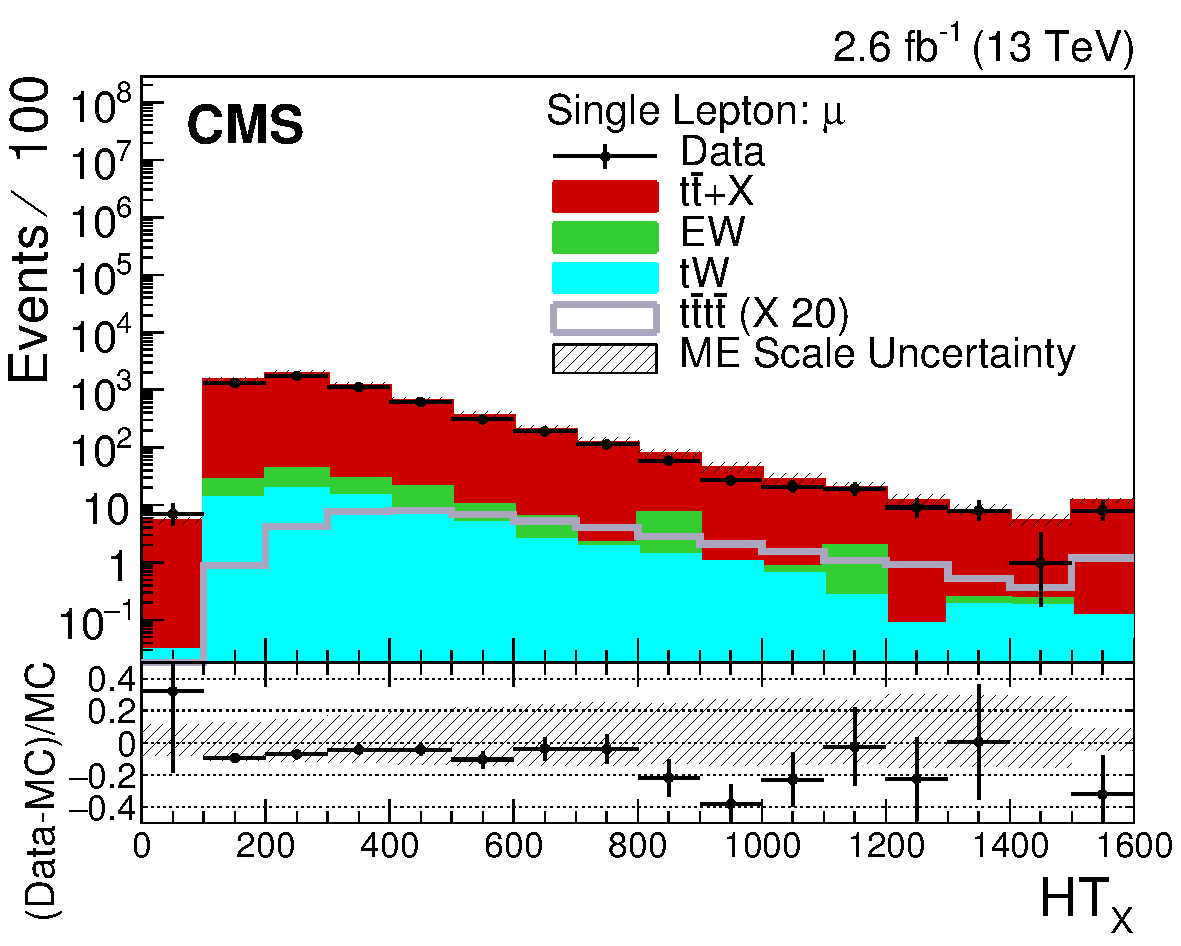
\includegraphics[width=0.48\textwidth]{images/Run2/HTX_StackLogY.pdf}
    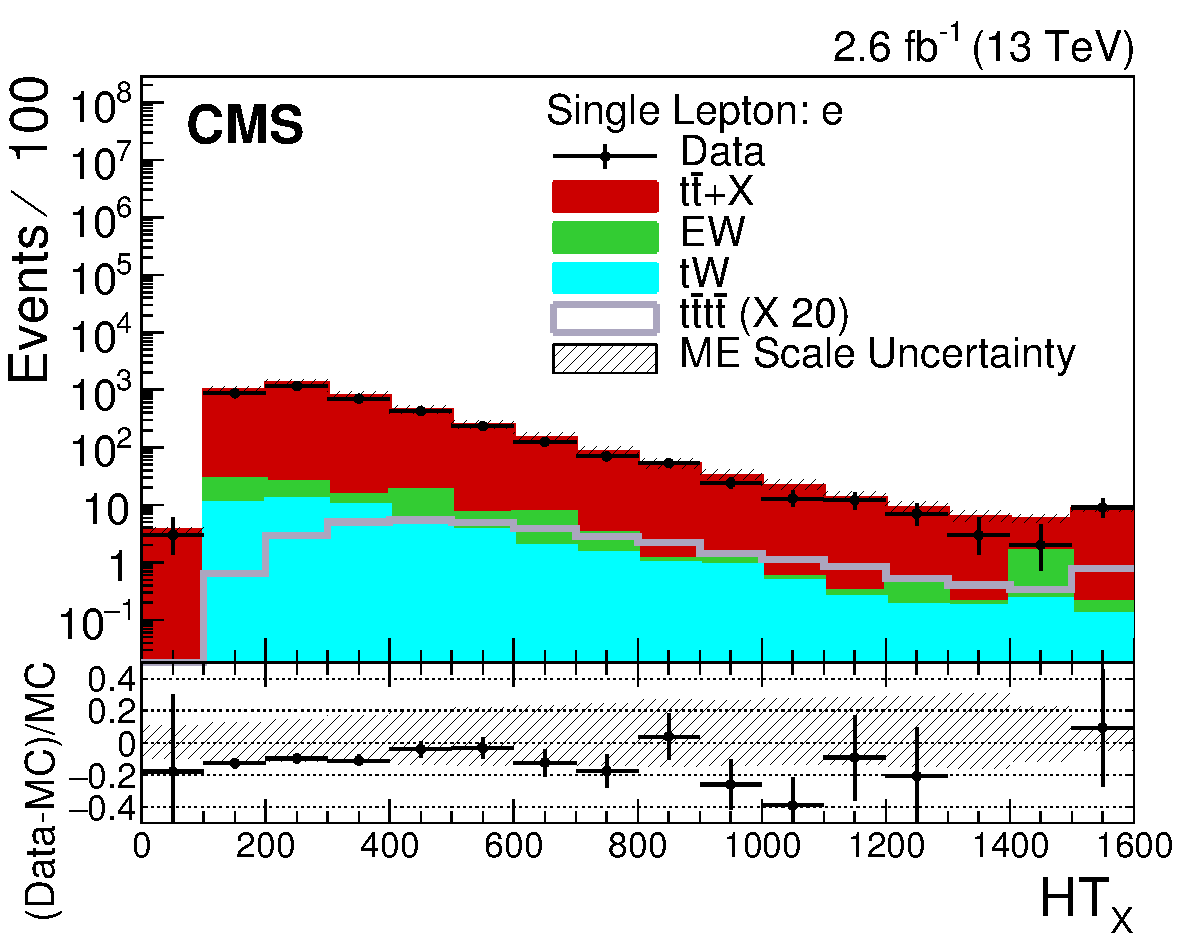
\includegraphics[width=0.48\textwidth]{images/Run2/HTX_StackLogY_e.pdf}
    \caption{The \HTX distributions for data and simulation in the $\mu$ + jets channel (left) and $e$ + jets channel (left).}
    \label{fig:HTX}
\end{figure} 

\begin{figure}
    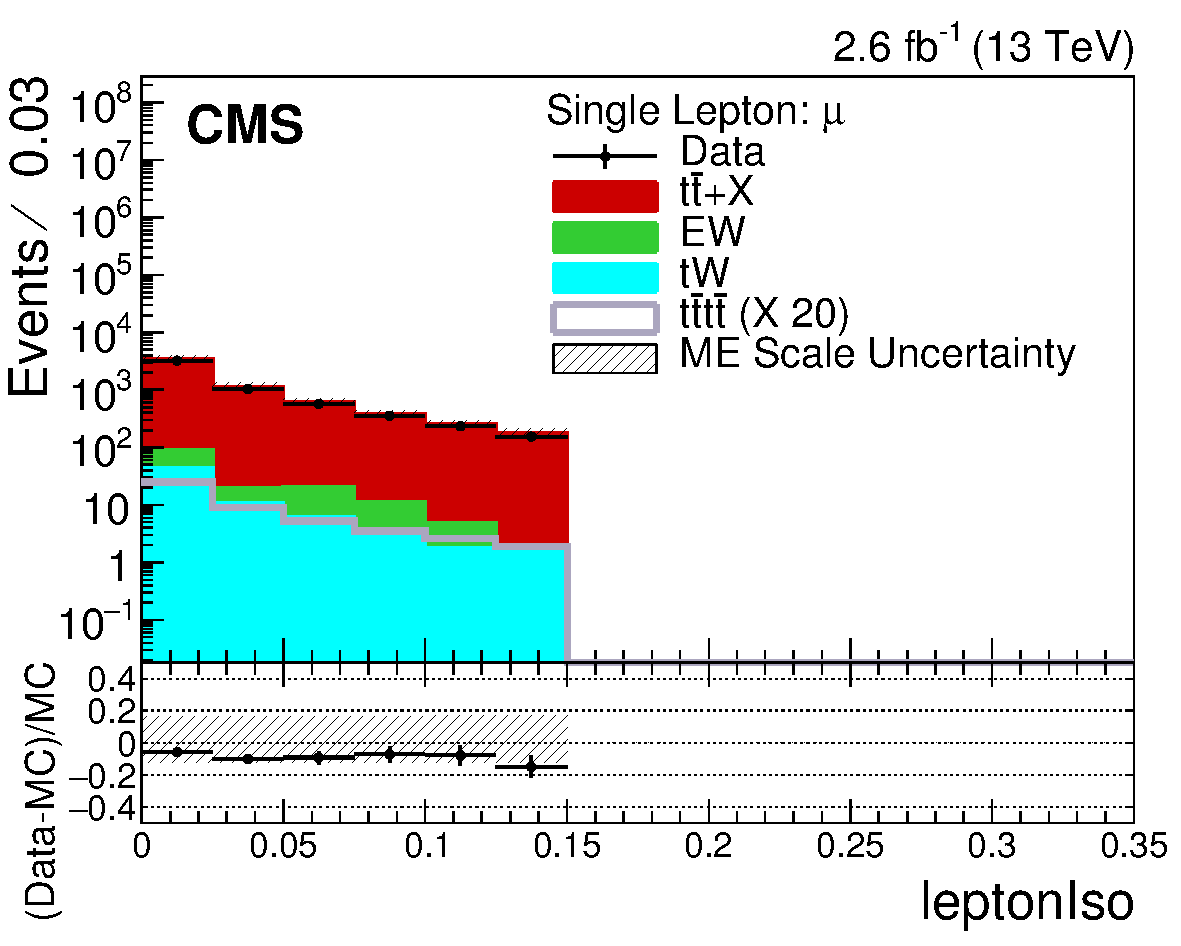
\includegraphics[width=0.48\textwidth]{images/Run2/leptonIso_StackLogY.pdf}
    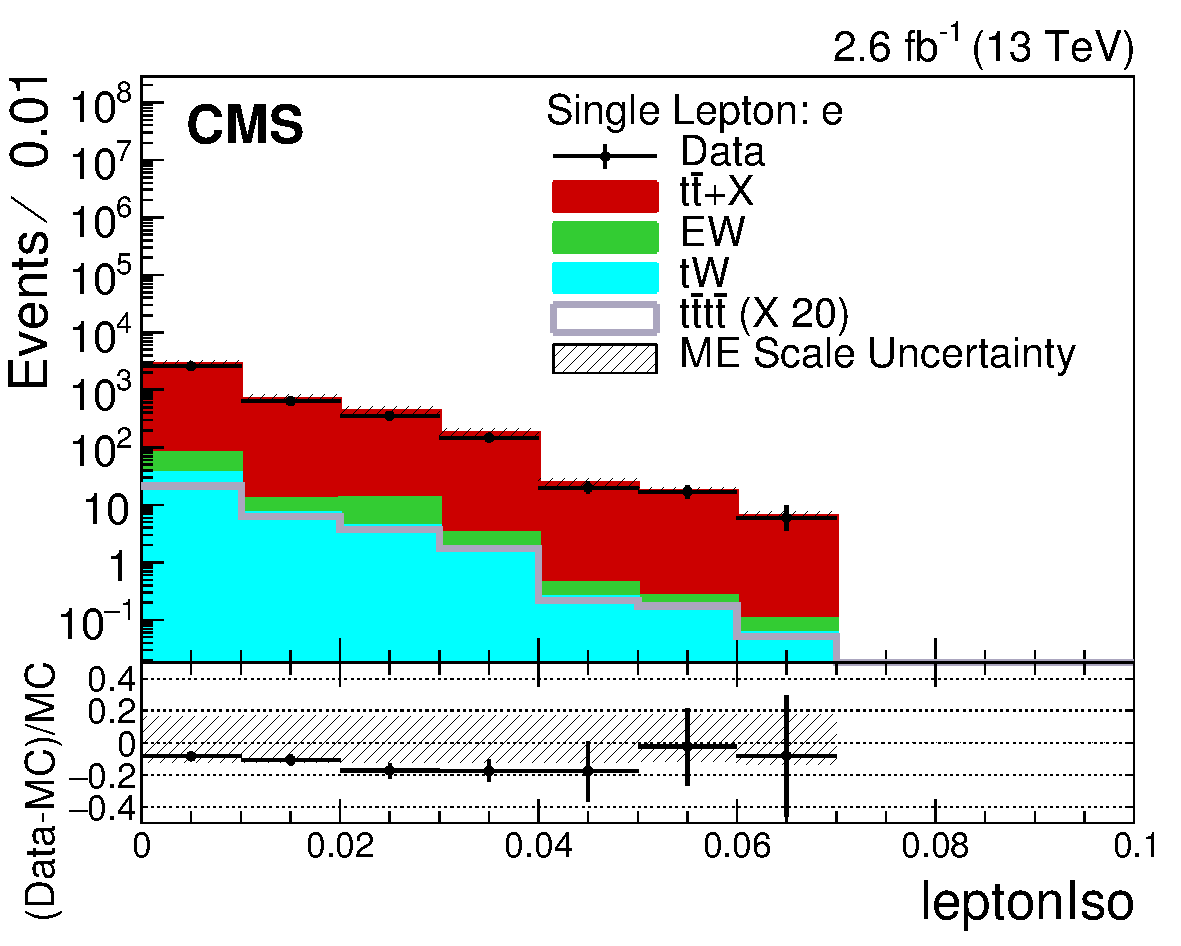
\includegraphics[width=0.48\textwidth]{images/Run2/leptonIso_StackLogY_e.pdf}
    \caption{The lepton isolation distributions for data and simulation in the $\mu$ + jets channel (left) and $e$ + jets channel (left) where the selection requirements on lepton isolation are evident.}
    \label{fig:lepiso}
\end{figure}
\pagebreak

\section{Discriminating between signal and background}
\label{sec:discriminating13}
It can be seen in Section~\ref{cutflow13} that the \ttbar background is three orders of magnitude larger than the \tttt signal in the signal region. The variables used to discriminate between \ttbar and \tttt are described below.
% There are three main features which can be used to discriminate; the number of top quarks which can be reconstructed in the event, the number of b-jets found in each event, and event activity such as \HT.

\subsection{Hadronic top quark content}
\label{sec:topContent13}
The hadronic top quark reconstruction, which is described in Section~\ref{sec:topreco}, is now discussed.

As the \antikt algorithm cannot resolve jets which have $\Delta R = \sqrt{  \eta^{2} + \phi^{2} } < 0.4$, a hadronically decaying top quark can only be deemed \emph{reconstructible} if the minimal $\Delta R$ between all three jets is $> 0.4$ which happens $> 98\%$ of the time in \ttbar and \tttt simulation when studying the decay products of the top quarks.\\
 % leptons and partons, and pairs of partons.\\
The BDT training was performed on 273~K \ttbar events. The input variables to the hadronic top quark reconstruction BDT are shown in Fig.~\ref{fig:TrijetBDTInputFeatures13}. The separation power for each of these variables and for the output BDT discriminator distribution in Fig.~\ref{fig:TrijetBDTOutput13} is evident as in the \runone studies in Chapter~\ref{c:Run1}. 

\begin{figure}[ht!]
\centering
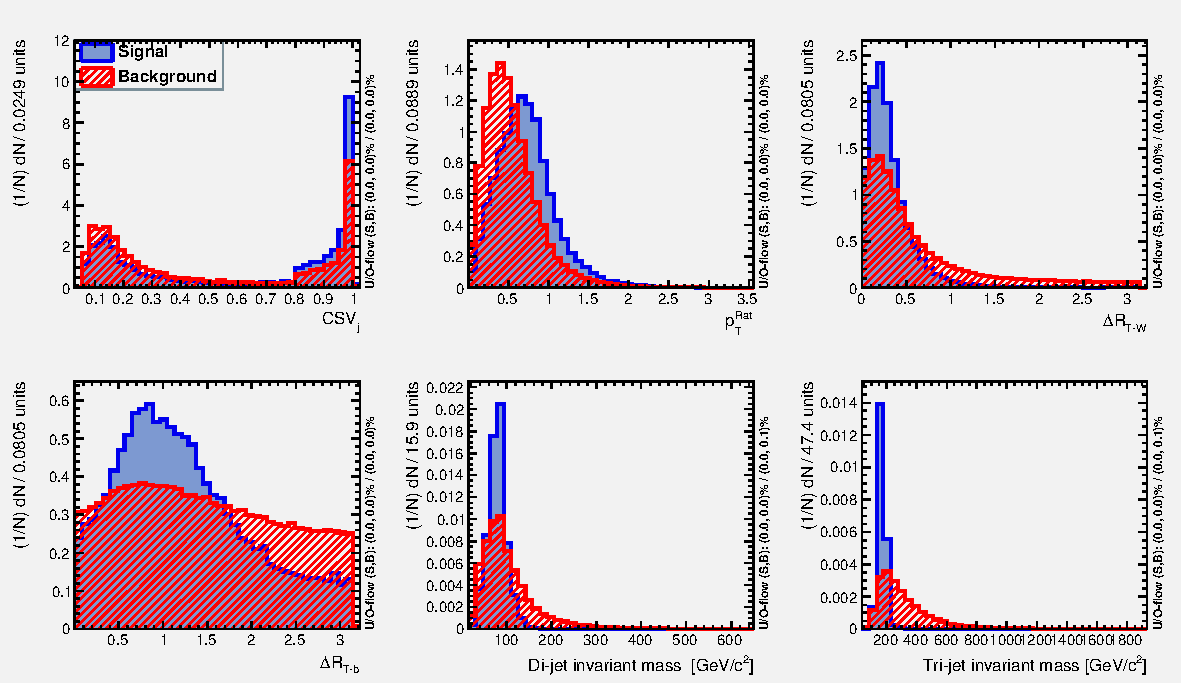
\includegraphics[width=\linewidth]{images/Run2/variables_id_c1.pdf}
\caption{Normalised distributions of the six variables used the MVA hadronic Top kinematic reconstruction are shown for good (hatched-red histograms) and bad (solid-blue histograms) trijets.}
\label{fig:TrijetBDTInputFeatures13}
\end{figure}

\begin{figure}[ht!]
\begin{center}
    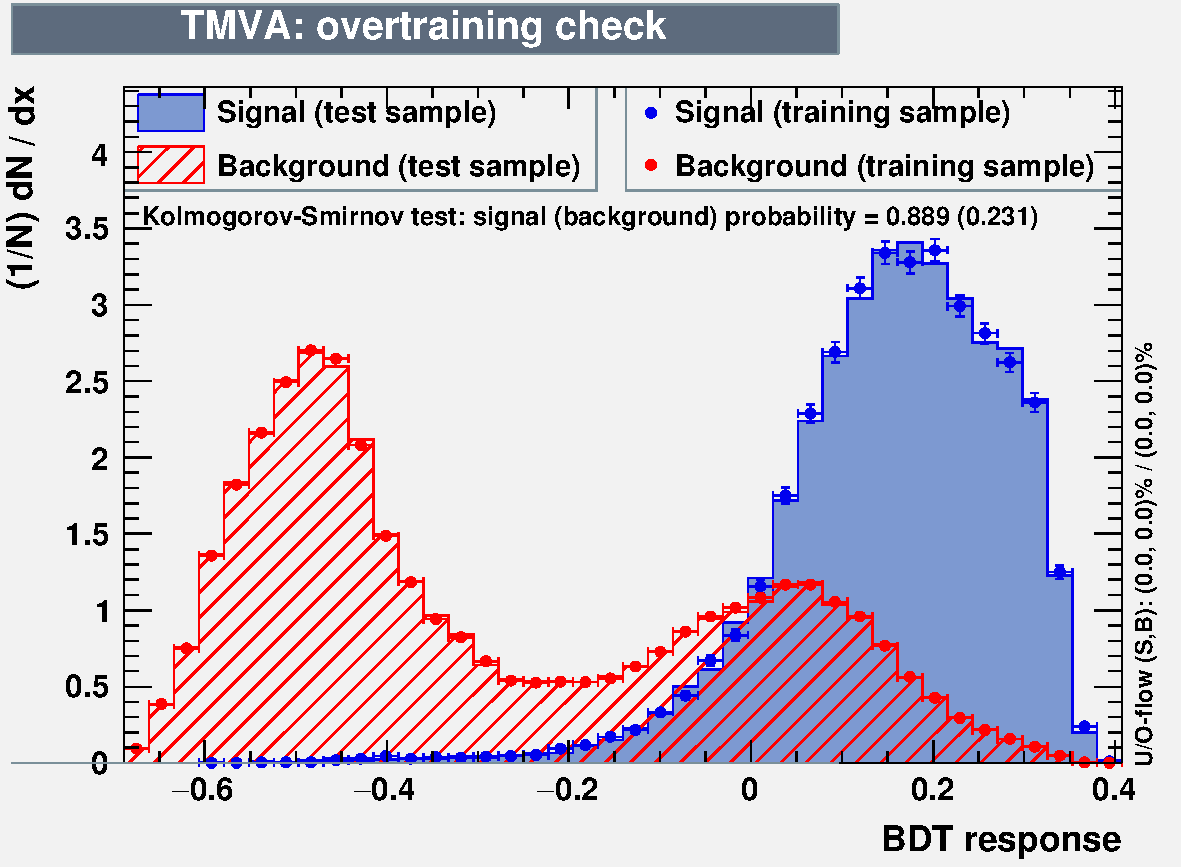
\includegraphics[width=0.55\textwidth]{images/Run2/overtrain_BDT.pdf}
    \caption{The discriminator distributions for the BDT classifier for good (solid blue) and bad (hatched-red) trijets in training and validation samples.}
    \label{fig:TrijetBDTOutput13}
\end{center}
\end{figure}

The effect of the tri-jet invariant mass variable in the BDT is shown in Fig.~\ref{fig:multimode13} where it can be clearly seen that this variable contributes to the strong splitting of the BDT output distribution at a value of $\approx-0.2$.

\begin{figure}[ht!]
\begin{center}
    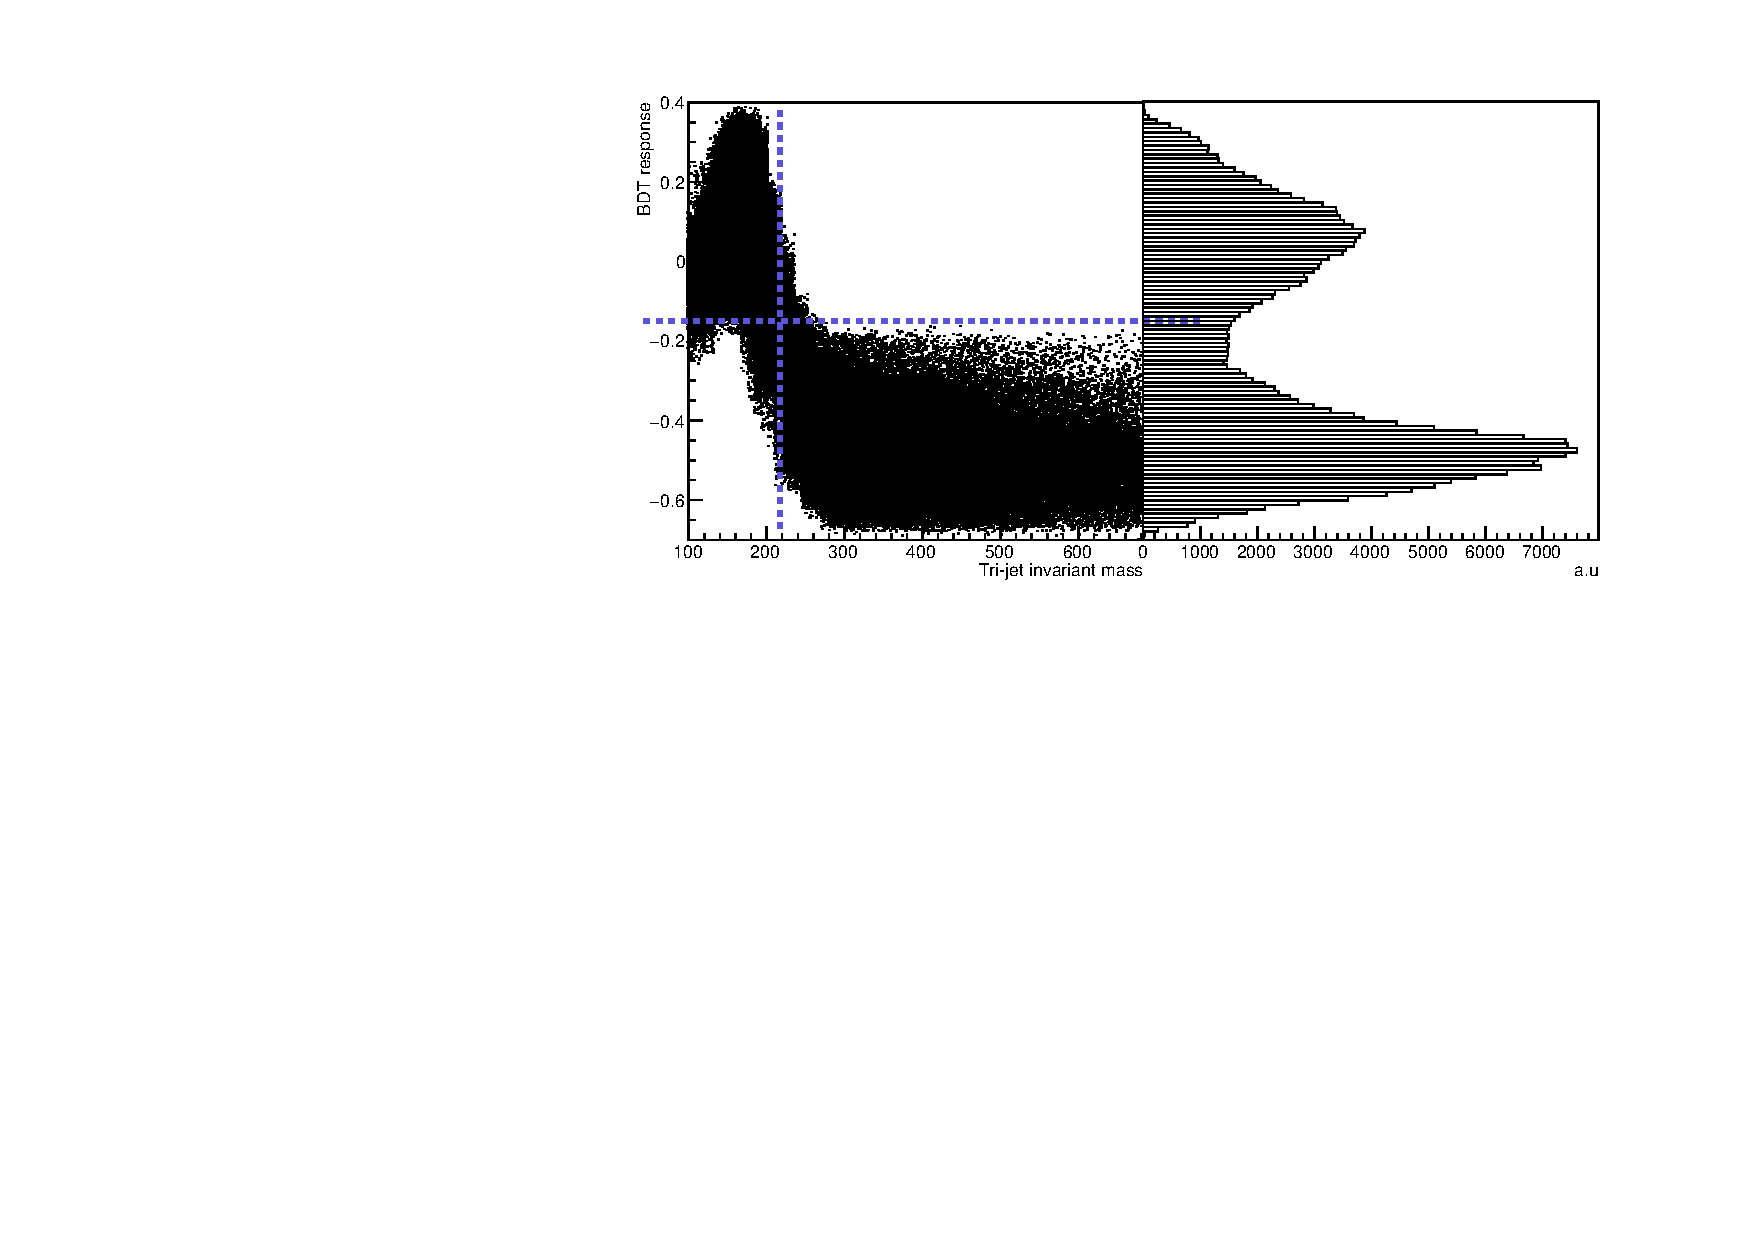
\includegraphics[width=0.85\textwidth]{images/Run2/multimode.pdf}
    \caption{The discriminator distributions for the BDT classifier versus trijet invariant mass and the projection on the vertical axis. Dashed lines indicate the cut value on trijet invariant mass at the BDT root node.}
    \label{fig:multimode13}
\end{center}
\end{figure}

Figure~\ref{fig:ContoursTopMassHadrWmass13}~(left) shows the distribution of good and bad tri-jet combinations in the phase space of tri-jet and di-jet invariant mass. It can be seen from Fig.~\ref{fig:ContoursTopMassHadrWmass13}~(right) that high BDT discriminator values are found in the region where the good tri-jet combinations are clustered at the top mass.
\begin{figure}[ht!]
\begin{center}
    \includegraphics[width=\textwidth]{images/Run2/ContoursHadrWmassTopMass.pdf}
    \caption{(Left)  Di-jet versus trijet invariant mass distribution for good (blue) and bad (red) trijet combination (Right) The average BDT response as a function of Di-jet versus trijet invariant mass input variables.}
    \label{fig:ContoursTopMassHadrWmass13}
\end{center}
\end{figure}

\subsubsection*{BDT$_{tri-jet2}$}

The BDT score of the second highest ranked tri-jet combination, BDT$_{tri-jet2}$ , as discussed in Section~\ref{sec:topreco}, is shown in Fig.~\ref{fig:bdtTrijet213}. There is good agreement between the data and simulation and sufficient discrimination power to be used in the event-level BDT.

\begin{figure}[ht!]
    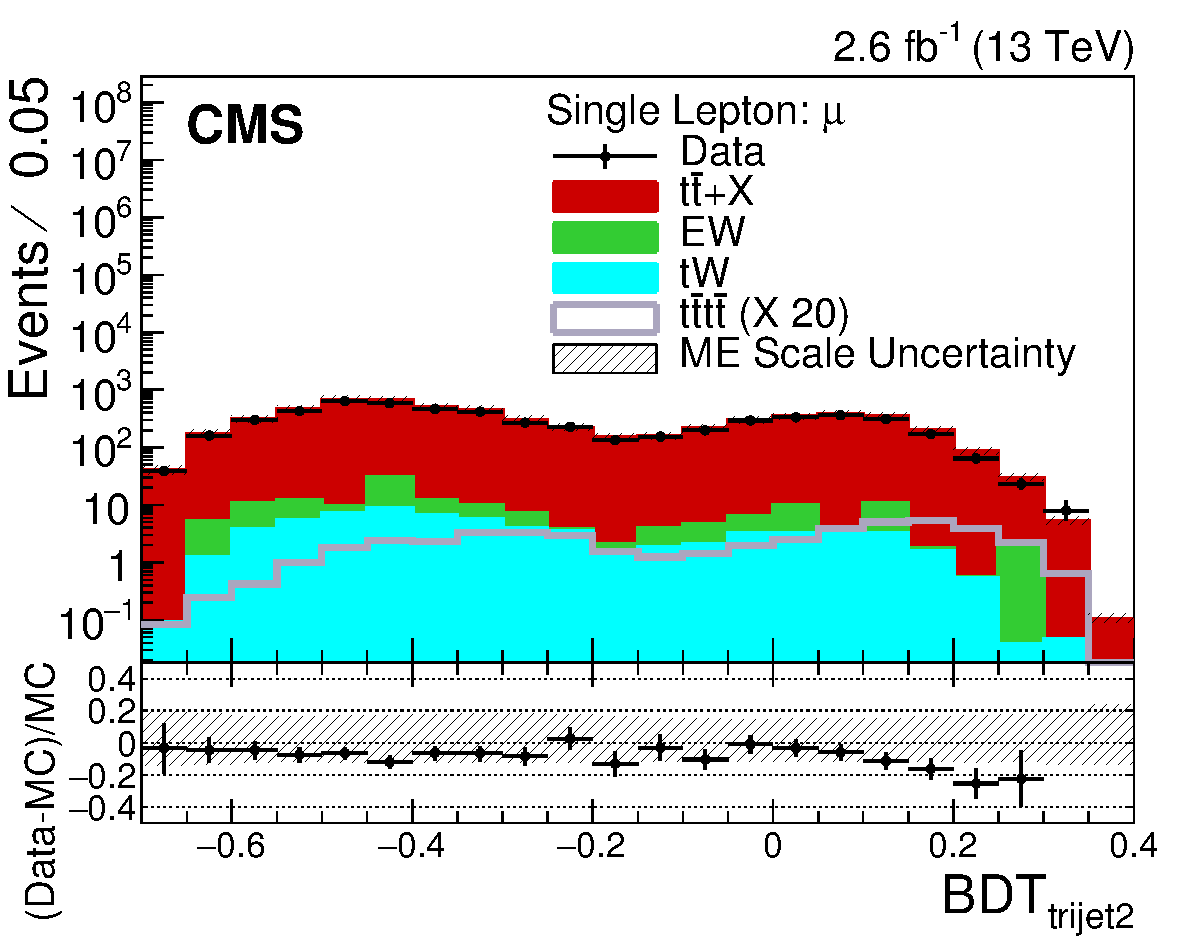
\includegraphics[width=0.44\textwidth]{images/Run2/BDT_trijet2_StackLogY.pdf}
    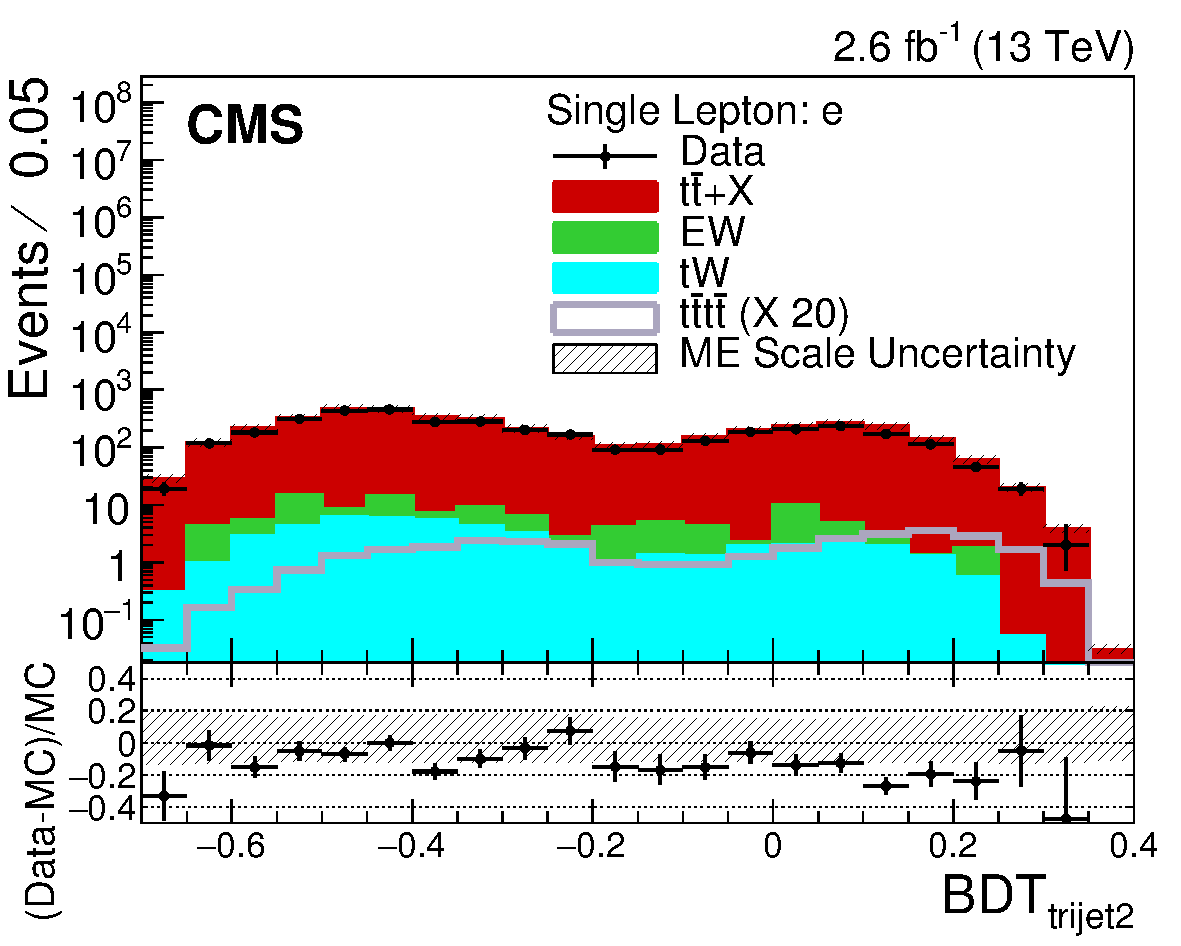
\includegraphics[width=0.44\textwidth]{images/Run2/BDT_trijet2_StackLogY_e.pdf}
    \caption{ The BDT$_{trijet2}$ distributions for data and simulation event in the $\mu$ + jets channel (left) and $e$ + jets channel (right).}
    \label{fig:bdtTrijet213}
\end{figure}

\subsubsection*{Reduced Event Variables}
The reduced variables formed from the reduced event, where the jets from the highest-ranked hadronic top quark have been removed from the collection of jets, are shown in Figs.~\ref{fig:htx13} and~\ref{fig:sumjetmassx13}. Again, good agreement is observed between the data and simulation and both variables were found to have good discrimination power in the event-level BDT.

\begin{figure}[ht!]
    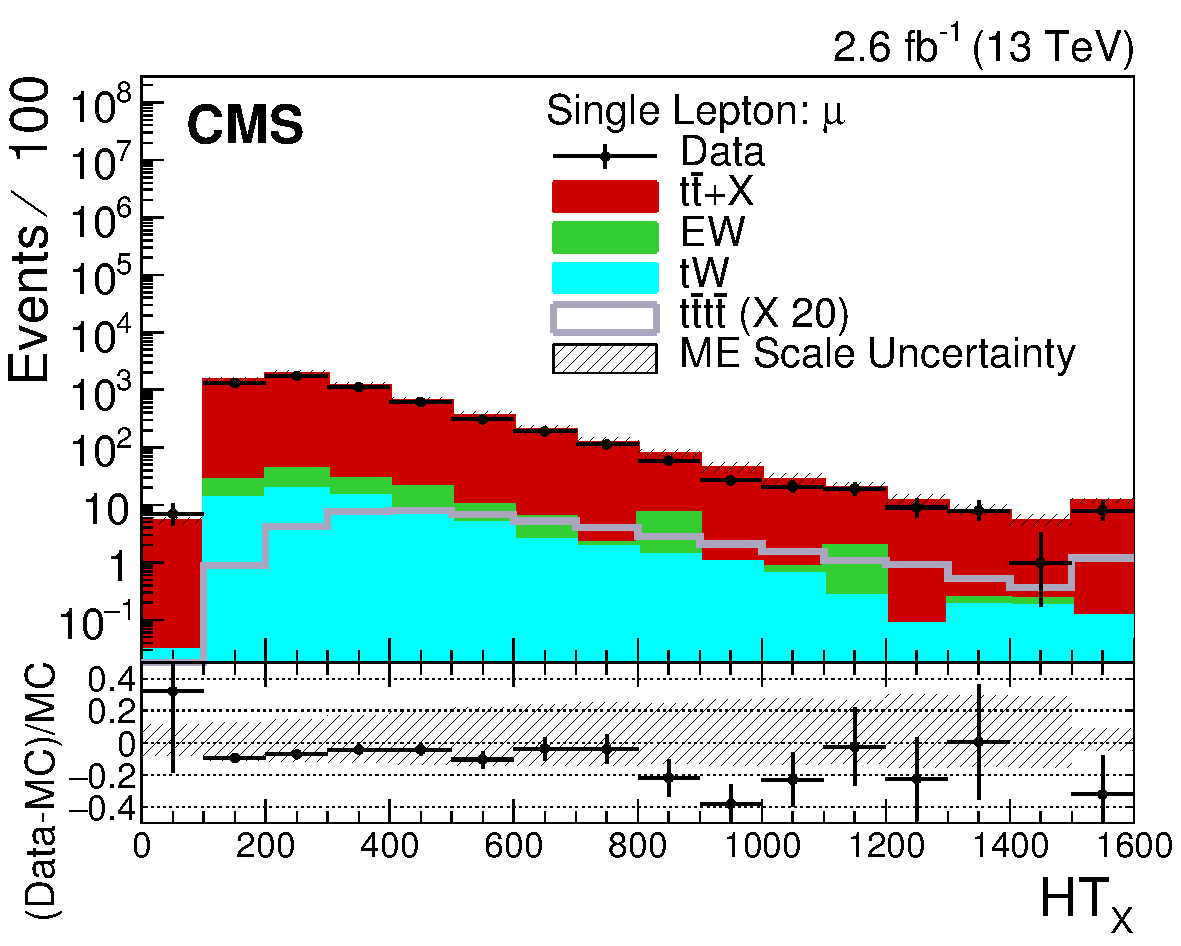
\includegraphics[width=0.44\textwidth]{images/Run2/HTX_StackLogY.pdf}
    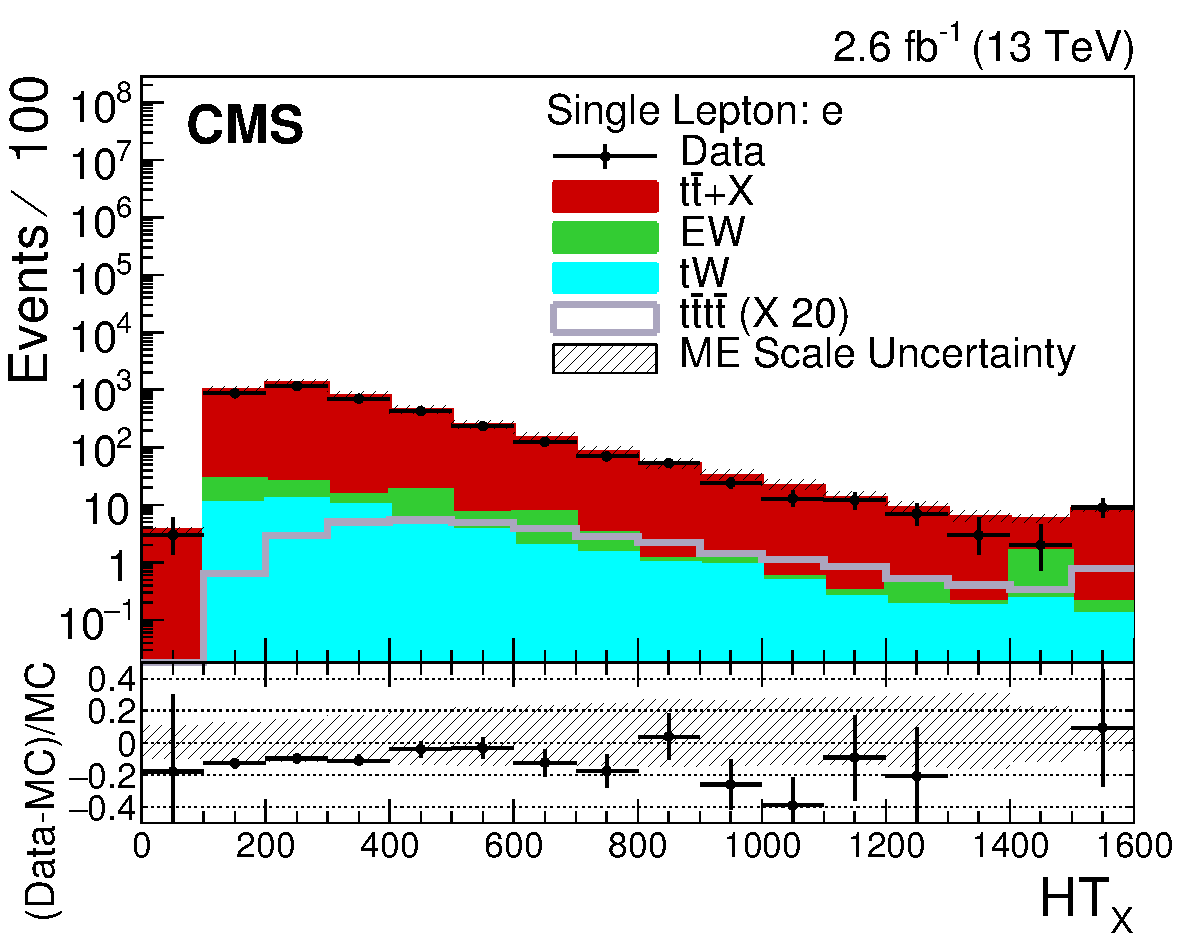
\includegraphics[width=0.44\textwidth]{images/Run2/HTX_StackLogY_e.pdf}
    \caption{ The \HTX distributions for data and simulation event in the $\mu$ + jets channel (left) and $e$ + jets channel (right).}
    \label{fig:htx13}
\end{figure}

\begin{figure}[ht!]
    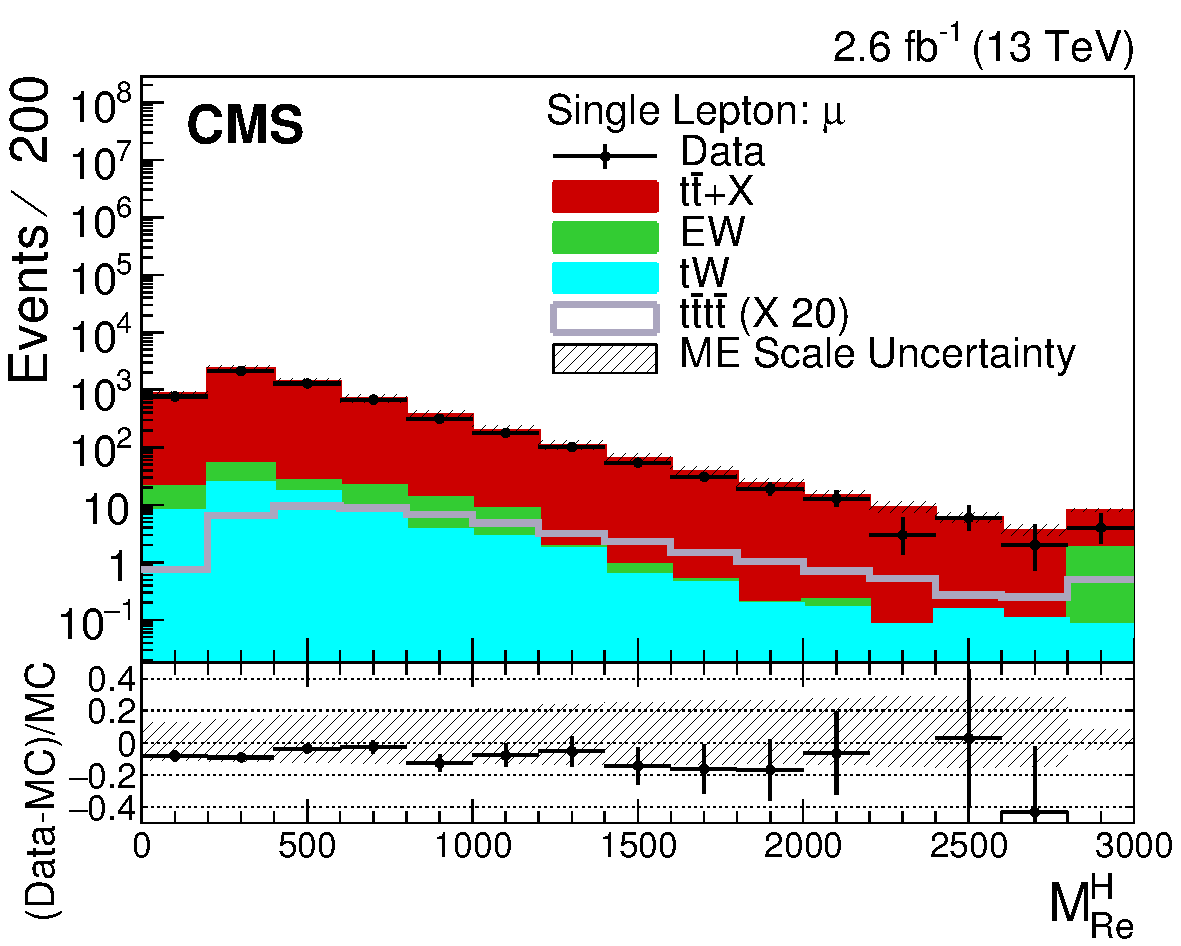
\includegraphics[width=0.44\textwidth]{images/Run2/SumJetMassX_StackLogY.pdf}
    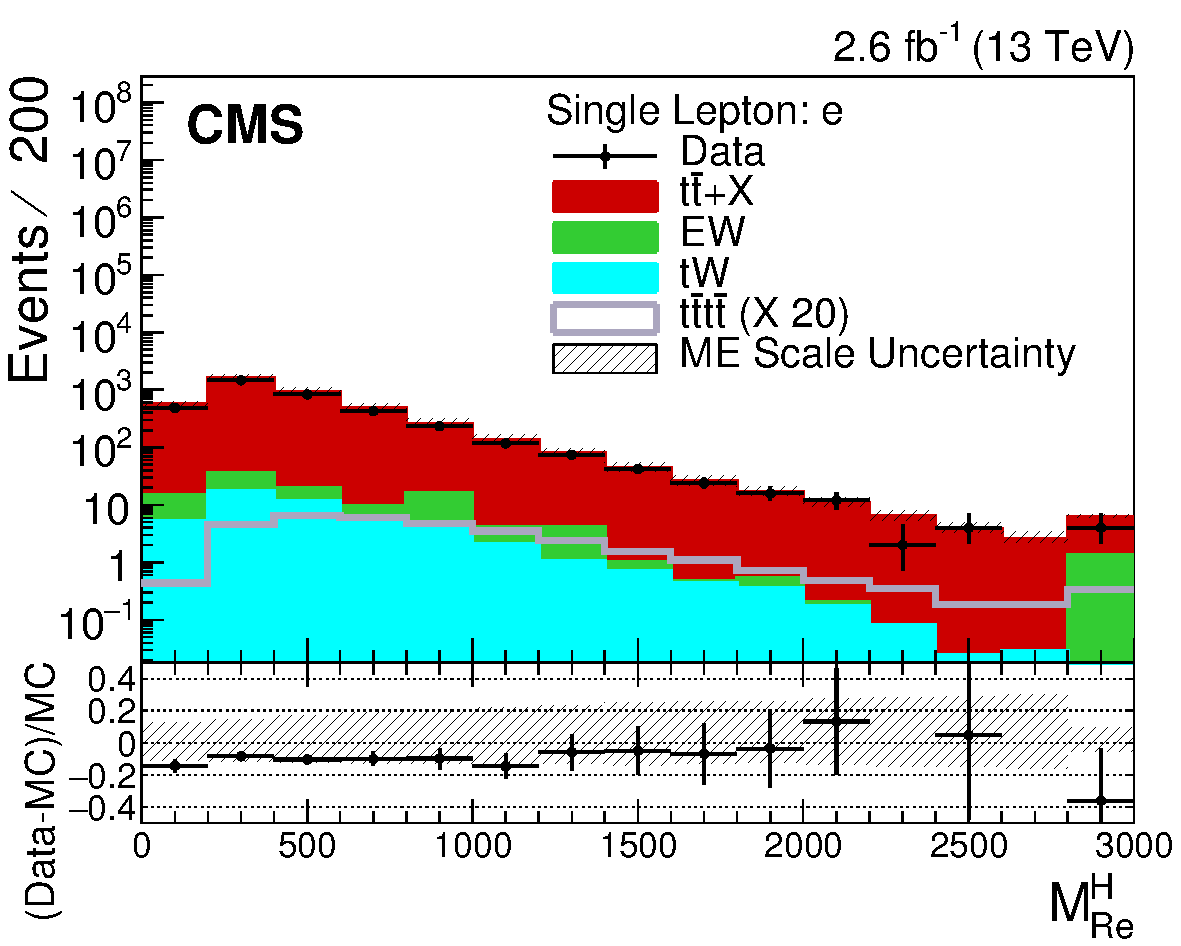
\includegraphics[width=0.44\textwidth]{images/Run2/SumJetMassX_StackLogY_e.pdf}
    \caption{ The \redhadmass distributions for data and simulation event in the $\mu$ + jets channel (left) and $e$ + jets channel (right).}
    \label{fig:sumjetmassx13}
\end{figure}


\subsection{Event activity and b-jet content variables chosen for the event-level BDT}
The following variables were chosen for their discrimination power within the event-level BDT and were previously described in Section~\ref{sec:Strategy}. It should be noted that the third-highest CSV and fourth-highest CSV values can be used in the $\sqrt{s} = 13$~TeV analysis as the CSV distributions have been corrected by the modelling in Section~\ref{subsec:method2btag}.


\begin{multicols}{2}
\setlength{\columnseprule}{0pt} 

\begin{itemize}
\item \htb
\item \htrat
\item \njets
\item lepton \pt, \leadleppt
\item \njetsw
\item third-highest CSV
\item fourth-highest CSV
\end{itemize}

\end{multicols}

\subsection{Event-level BDT}
A \ttbar sample and a \tttt sample are provided to the TMVA package to train and test the performance of the event-level BDT using the AdaBoost boosting algorithm~\cite{FREUND1997119}. The \MADGRAPH\aMCATNLO \tttt sample was used with all negative weights set to one in the training. The gradient boosting algorithm~\cite{mason1999boosting} can be used with negative weights, hence it was used to verify that the inclusion of negative weights had negligible impact on the final limit compared to set all weights to unity (See Appendix~\ref{app:gradBoost}). Ultimately the AdaBoost algorithm produced a stronger expected limit on the \tttt cross section than the gradient boosting algorithm with the negative weights set to one so it was the algorithm of choice for this analysis. The jet modelling scale factor weight from Section~\ref{subsec:alphaS} is supplied to the BDT as it is important to correct the mismodelling of the most powerful variable input into the BDT.\\
The separation of the input variables, before any boost weights are applied, is shown in Fig.~\ref{fig:BDTInputVars} and the ranking of the variables in terms of variable importance are shown for the muon channel in Table~\ref{tab:BDTrankings}. The variables \njets, third-highest CSV and \htrat are the highest ranked variables and their discriminating power is evident in their initial separation power. The lowest ranked variable is \leadleppt, which is also seen in Fig.~\ref{fig:BDTInputVars} to have poor separation power initially. However it still enhances the discrimination power of the BDT to include the \leadleppt variable and it is preferable to have at least one leptonic variable in the list of input variables rather than all hadronic variables.

\begin{figure}[h!]
    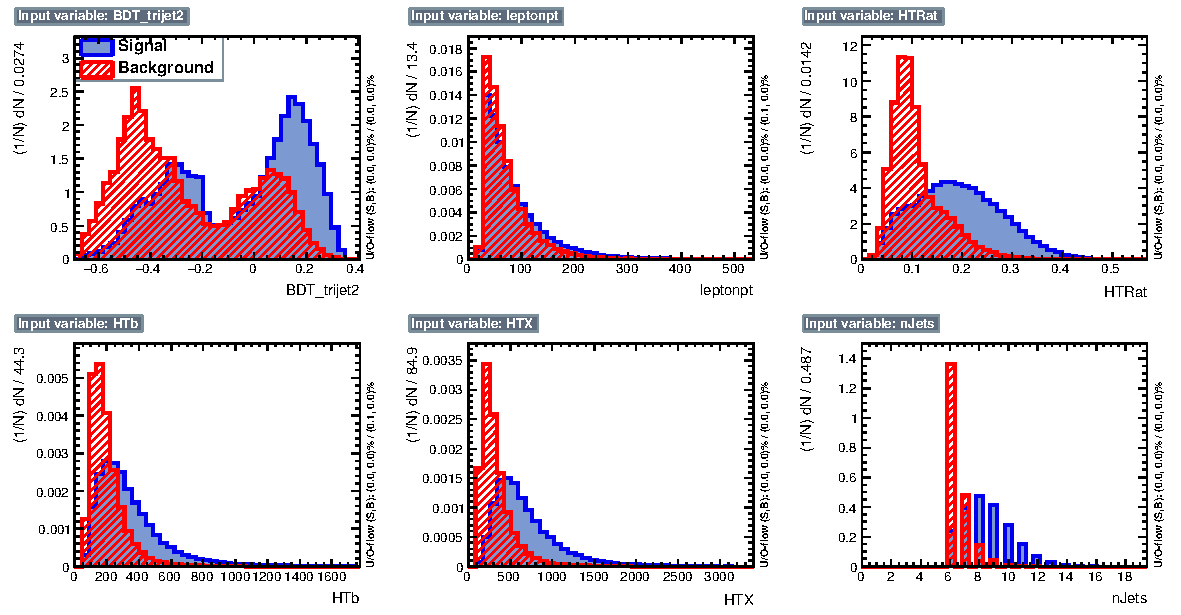
\includegraphics[width=\textwidth]{images/Run2/variables_id_c1_ELBDT13.pdf}\\
    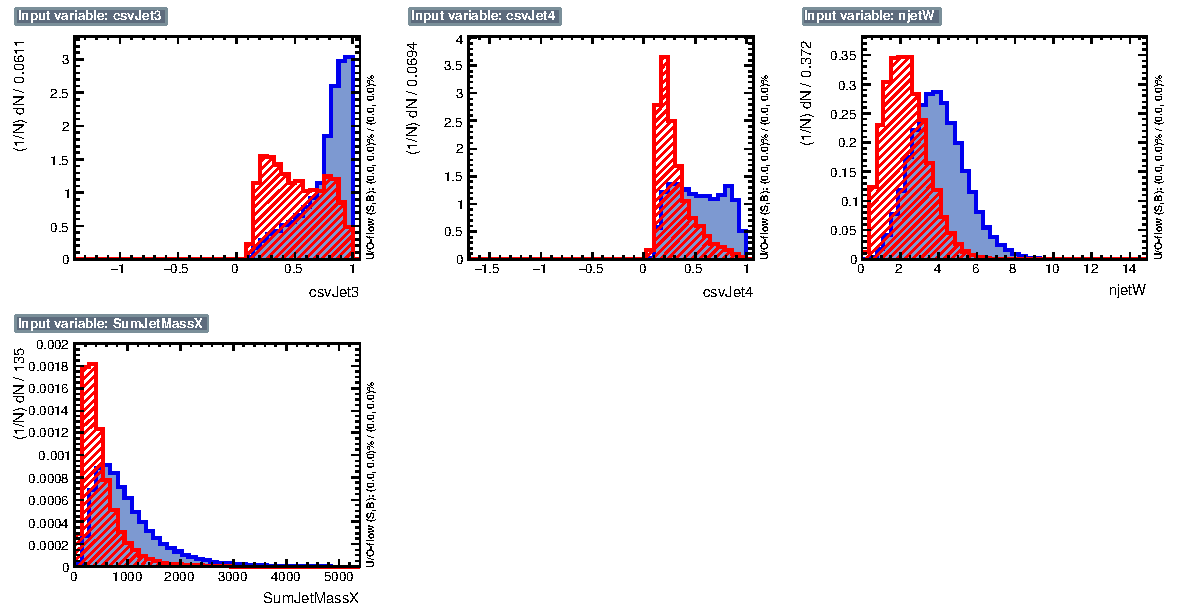
\includegraphics[width=\textwidth]{images/Run2/variables_id_c2_ELBDT13.pdf}
    \caption{Normalised distributions of the input variables in the muon channel taken from TMVA}
    \label{fig:BDTInputVars}
\end{figure}

\begin{table}[ht!]
\centering
\begin{tabular}{| l | l | l | p{5cm} |}
  \hline
Rank & Variable & Importance \\
 \hline
1 & \njets & 1.340e-01\\
2 & third-highest CSV &1.180e-01\\
3 & \htrat & 1.133e-01\\
4 & BDT$_{trijet2}$ & 1.091e-01 \\
5 & \njetsw &1.082e-01\\
6 & \redhadmass& 1.026e-01\\
7 & \HTX & 9.867e-02\\
8 & \htb & 8.650e-02 \\
9 & fourth-highest CSV & 7.630e-02\\
10 & \leadleppt & 5.334e-02  \\
\hline
\end{tabular}
 \caption{Ranking of variables in order of discrimination power within the BDT.}
  \label{tab:BDTrankings}
  \end{table}

The output discriminator value for the event level BDT is split into \njets categories of 6, 7, 8 and $\geq$9 jets . Further to the \runone analysis in Chapter~\ref{c:Run1}, the distributions are also split into \nMtags categories of 2, 3 and $\geq$4 b-tags which further categorises the distributions into regions which are more sensitive to the signal and regions which are better for constraining the background.
The output BDT plots are shown for the $\njets=6$ and $\nMtags=2$ category in Fig.~\ref{fig:BDT_Mu29Aug400trees_5MinNodeSize_20nCuts_3MaxDepth_5adaboostbeta_adaBoost_alphaSTune_noMinEvents62}, which has a large background to signal ratio. Comparatively in the $\njets=6$ and $\nMtags=3$ category and $\njets=6$ and $\nMtags\geq4$ category, in Figs.~\ref{fig:BDT_Mu29Aug400trees_5MinNodeSize_20nCuts_3MaxDepth_5adaboostbeta_adaBoost_alphaSTune_noMinEvents93} and~\ref{fig:BDT_Mu29Aug400trees_5MinNodeSize_20nCuts_3MaxDepth_5adaboostbeta_adaBoost_alphaSTune_noMinEvents94} respectively, it can be seen that the background contribution is a lot smaller and there is better separation between signal and background. The other BDT categories can be found in Appendix~\ref{app:BDTtemp}.
 % in Figs.~\ref{fig:BDT_Mu29Aug400trees_5MinNodeSize_20nCuts_3MaxDepth_5adaboostbeta_adaBoost_alphaSTune_noMinEvents62}~-~\ref{fig:BDT_Mu29Aug400trees_5MinNodeSize_20nCuts_3MaxDepth_5adaboostbeta_adaBoost_alphaSTune_noMinEvents94}. It can be seen that the signal becomes more separated from the background in the higher \njets and \nMtags categories as it moves towards higher BDT discriminator values.
The lower \njets and \nMtags categories are still included as they can be used to help to constrain the \ttbar background. These categories act like control regions due to the very large background to signal ratio. 

\begin{figure}[ht!]
    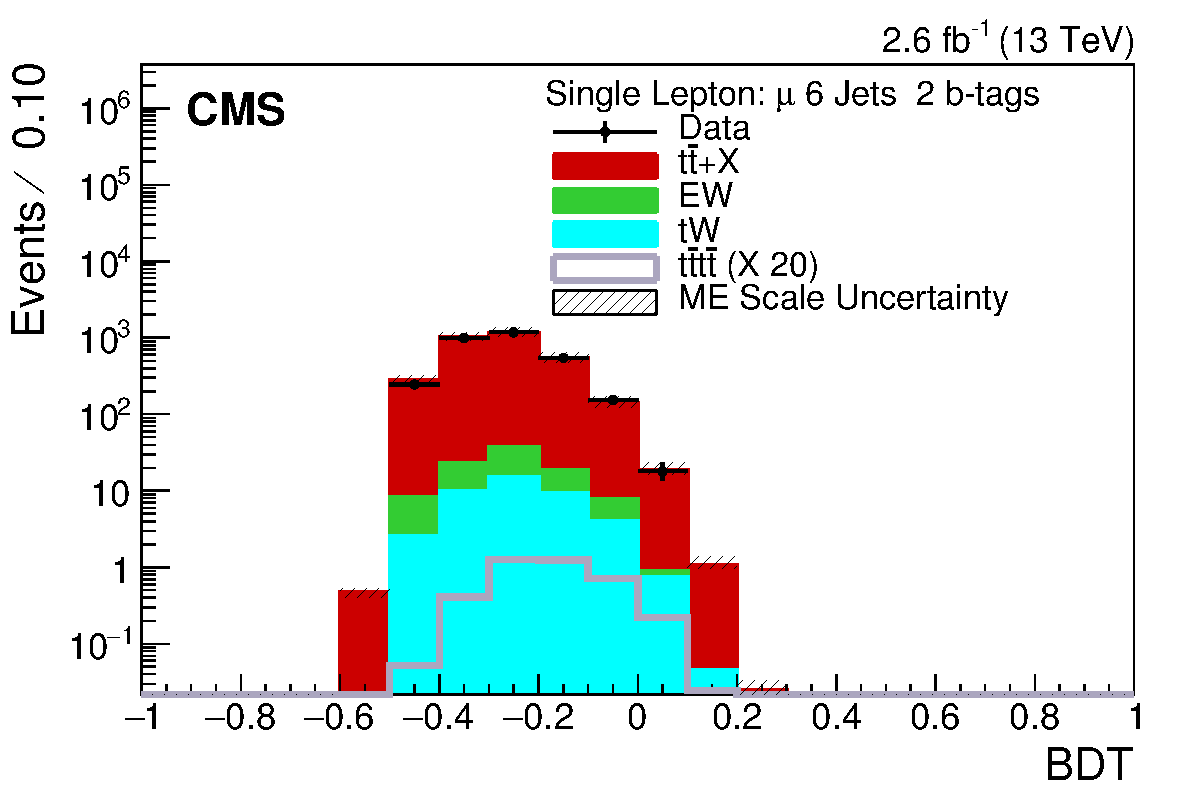
\includegraphics[width=0.48\textwidth]{images/Run2/BDT_Mu29Aug400trees_5MinNodeSize_20nCuts_3MaxDepth_5adaboostbeta_adaBoost_alphaSTune_noMinEvents6nJets2nMtags_StackLogY.pdf}
    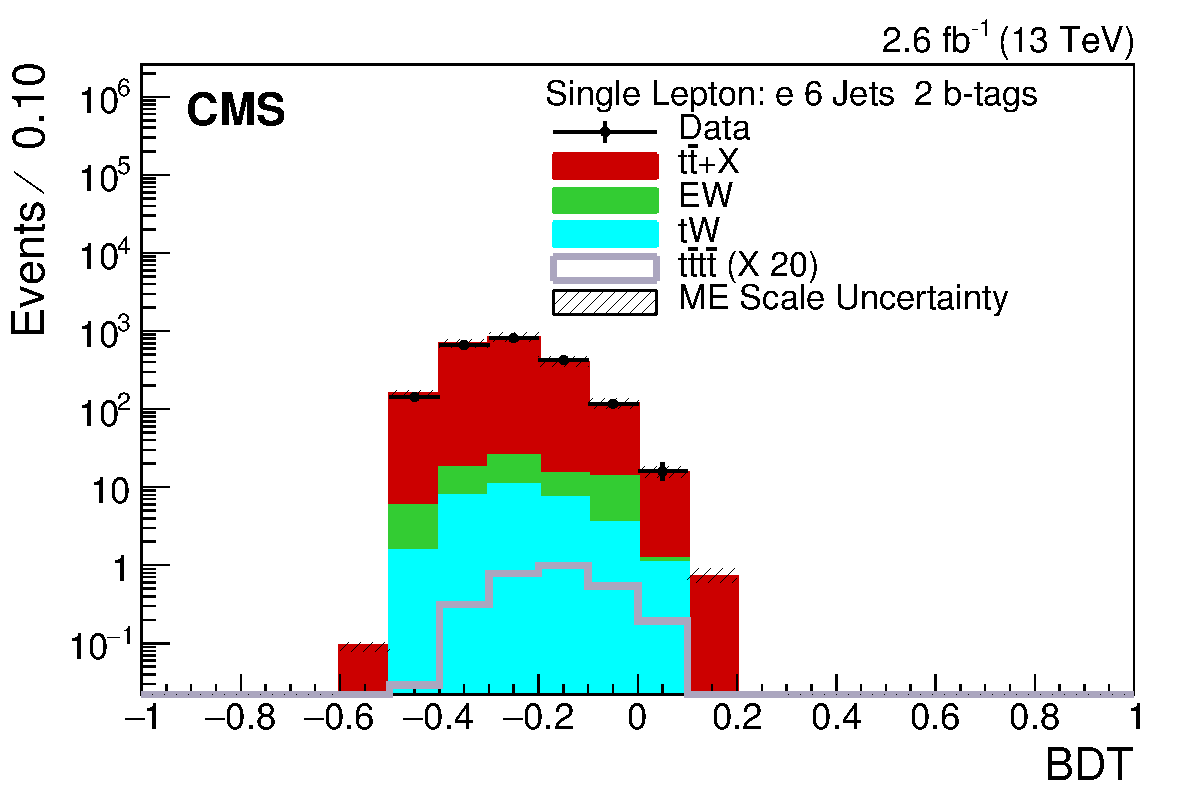
\includegraphics[width=0.48\textwidth]{images/Run2/BDT_El29Aug400trees_5MinNodeSize_20nCuts_3MaxDepth_5adaboostbeta_adaBoost_alphaSTune_noMinEvents6nJets2nMtags_StackLogY.pdf} 
    \caption{The BDT output distributions for AdaBoost for data and simulation in the $\mu$ + jets channel (left) and e + jets channel (left) are shown for the 6 \njets and 2\nMtags category.}
    \label{fig:BDT_Mu29Aug400trees_5MinNodeSize_20nCuts_3MaxDepth_5adaboostbeta_adaBoost_alphaSTune_noMinEvents62}
\end{figure}

\begin{figure}[ht!]
    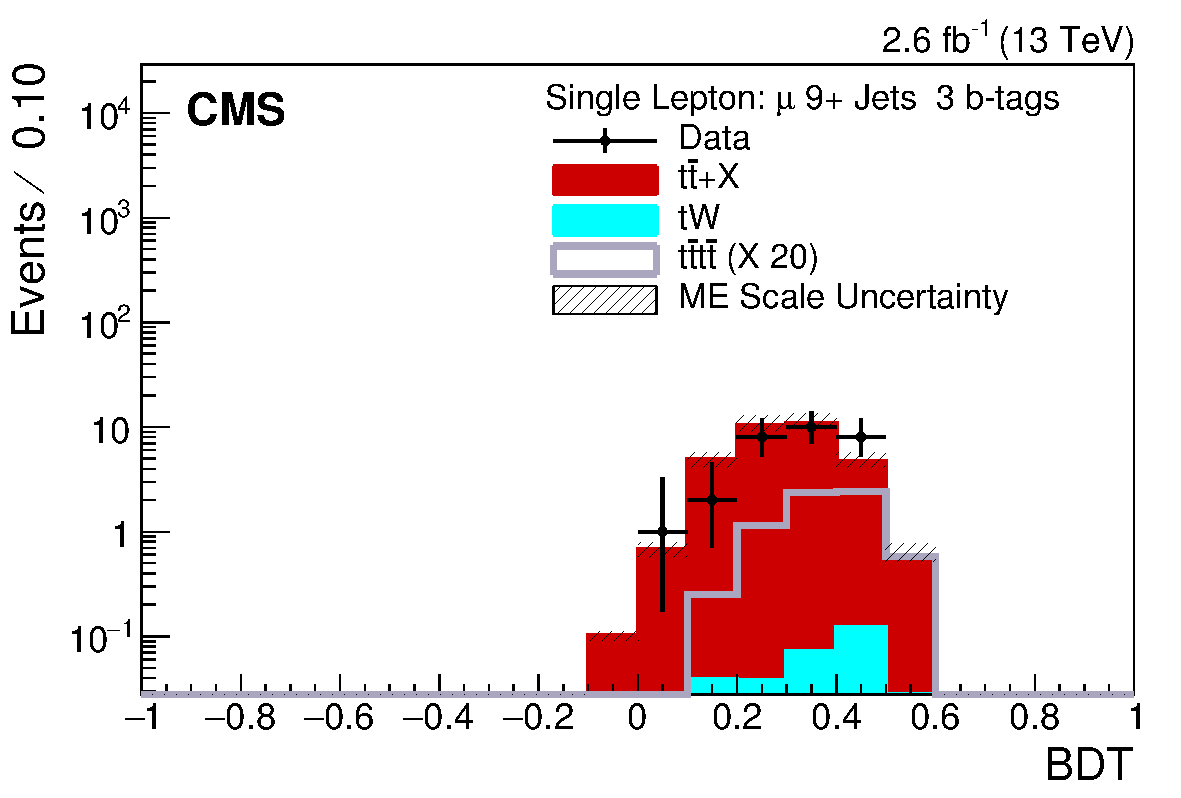
\includegraphics[width=0.48\textwidth]{images/Run2/BDT_Mu29Aug400trees_5MinNodeSize_20nCuts_3MaxDepth_5adaboostbeta_adaBoost_alphaSTune_noMinEvents9nJets3nMtags_StackLogY.pdf}
    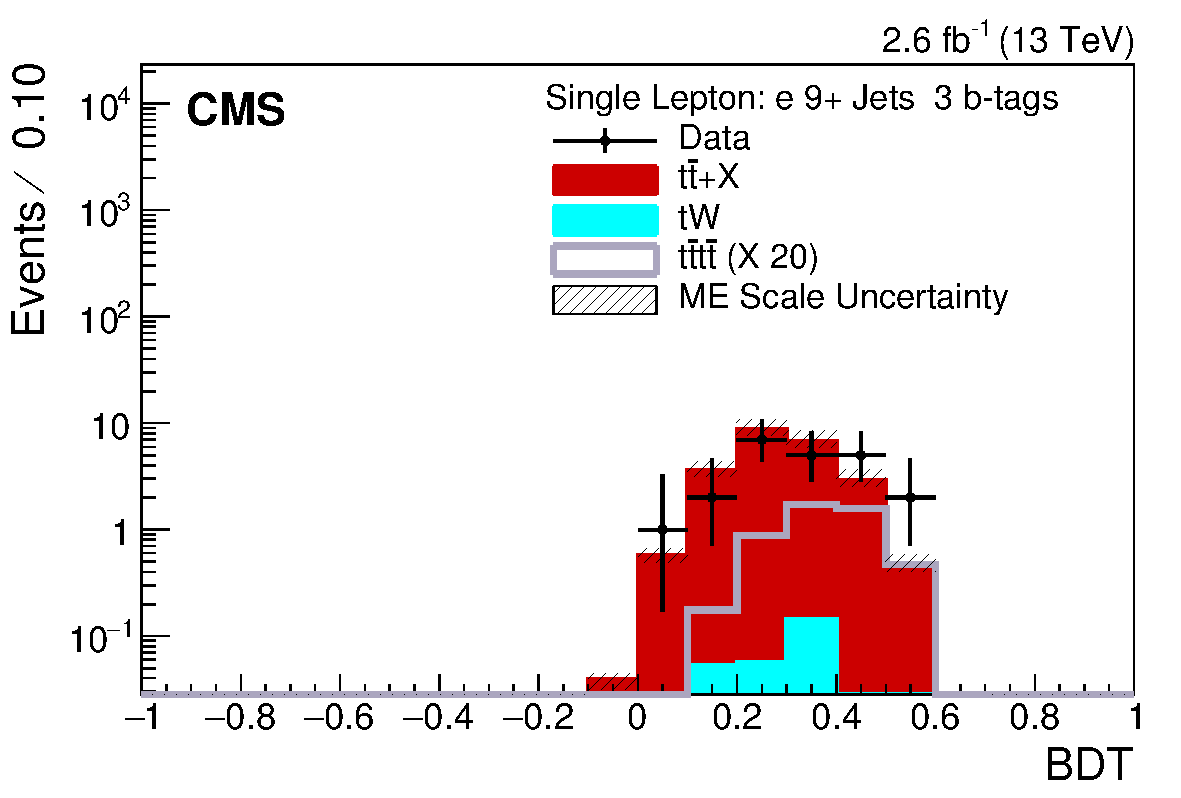
\includegraphics[width=0.48\textwidth]{images/Run2/BDT_El29Aug400trees_5MinNodeSize_20nCuts_3MaxDepth_5adaboostbeta_adaBoost_alphaSTune_noMinEvents9nJets3nMtags_StackLogY.pdf}
    \caption{The BDT output distributions for AdaBoost for data and simulation in the $\mu$ + jets channel (left) and $e$ + jets channel (left) are shown for the $\geq9$ \njets  and 3 \nMtags category.}
    \label{fig:BDT_Mu29Aug400trees_5MinNodeSize_20nCuts_3MaxDepth_5adaboostbeta_adaBoost_alphaSTune_noMinEvents93}
\end{figure}

\begin{figure}[ht!]
    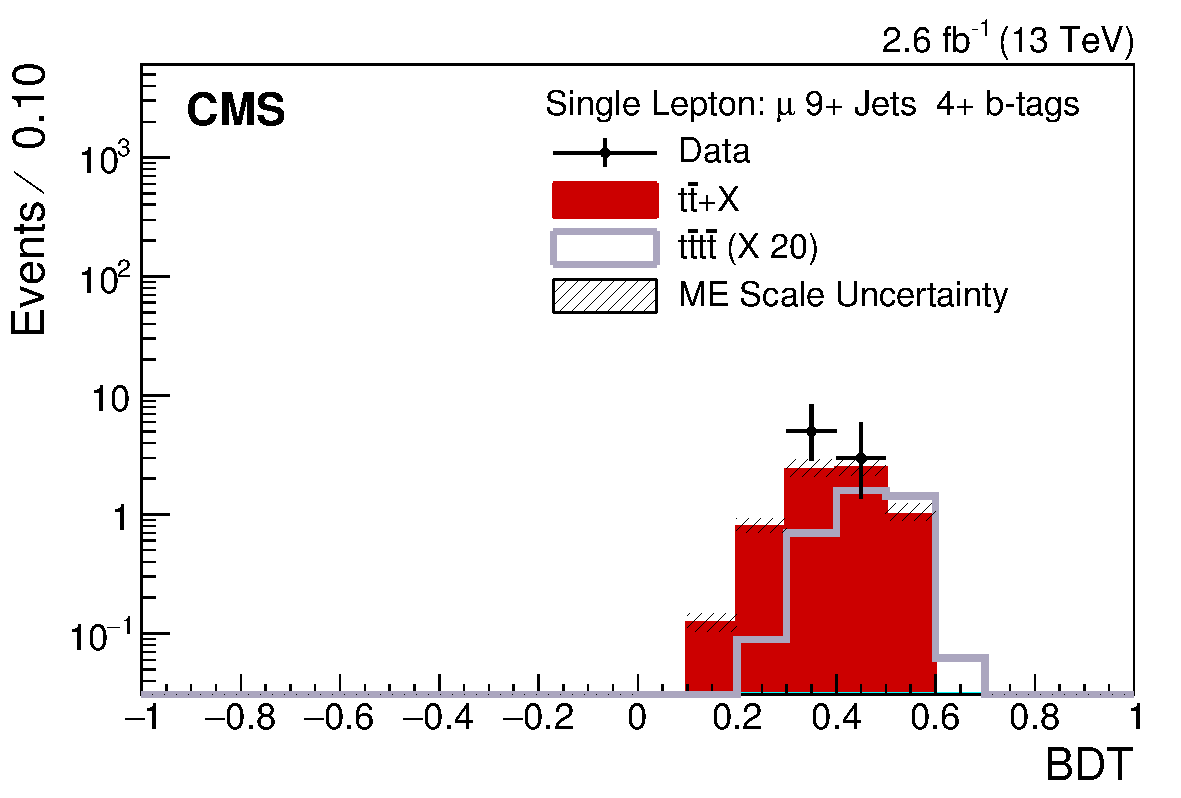
\includegraphics[width=0.48\textwidth]{images/Run2/BDT_Mu29Aug400trees_5MinNodeSize_20nCuts_3MaxDepth_5adaboostbeta_adaBoost_alphaSTune_noMinEvents9nJets4nMtags_StackLogY.pdf}
    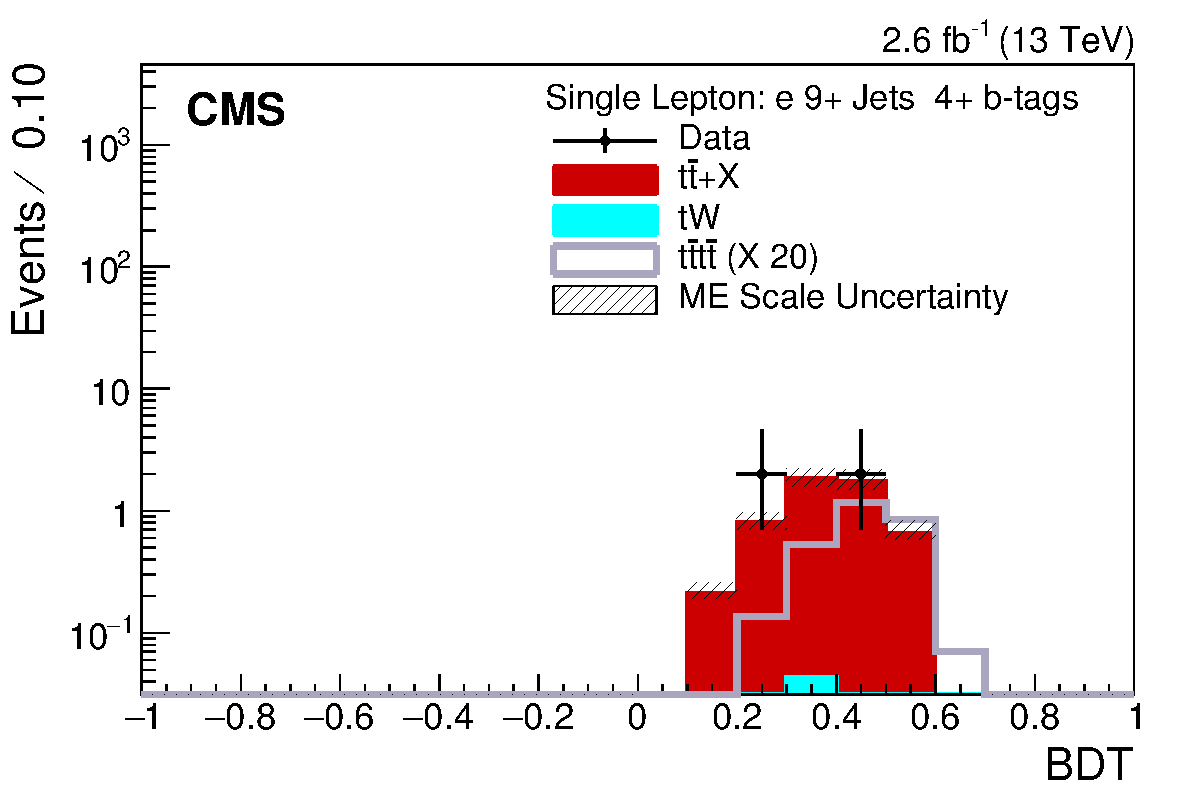
\includegraphics[width=0.48\textwidth]{images/Run2/BDT_El29Aug400trees_5MinNodeSize_20nCuts_3MaxDepth_5adaboostbeta_adaBoost_alphaSTune_noMinEvents9nJets4nMtags_StackLogY.pdf}    
    \caption{The BDT output distributions for AdaBoost for data and simulation in the $\mu$ + jets channel (left) and $e$ + jets channel (right) are shown for the $\geq9$ \njets and $\geq4$ \nMtags category.}
    \label{fig:BDT_Mu29Aug400trees_5MinNodeSize_20nCuts_3MaxDepth_5adaboostbeta_adaBoost_alphaSTune_noMinEvents94}
\end{figure}

\subsubsection{Stability of the event-level BDT}

The BDT was seen to be very stable with respect to changes in the number of trees used and to the minimum number of events required at a node for further splitting to occur. The impact on the final expected limit was negligible when changing these BDT hyperparameters. Training was also performed in jet categories of 6-7 jets and $\geq$8 jets separately to study whether a separate training in the $\geq8$ jets category would improve the power of the BDT to separate \ttbar and \tttt events in a signal-rich region. However the expected limit derived from this alternative training was not enhanced with respect to the inclusive training in all jet categories. The most significant improvement in the expected limit comes from optimising the \njets and \nMtags categories. Further categorisation into higher \njets and \nMtags categories improves the expected limit however these categories become very statistically limited with 2.6~\fbinv of data.

\subsubsection{Correlation matrices for BDT input variables}

% The correlation matrices for signal and background are shown in Fig.~\ref{fig:corrMat}. The largest correlation exists between \njetsw and \redhadmass. This is not surprising as \njetsw takes into account the weight of jets above a pt threshold and \redhadmass is the invariant mass of the reduced event. Many high pt jets in an event will correspond to a larger value of \redhadmass. 
% Correlated variables are handled well within a BDT and that was one of the reasons for the choice of this type of multivariate algorithm. The correlation matrices were used at an earlier stage in the analysis to assess what variables were very highly correlated and could be removed from the input BDT variables as they would serve little use within the BDT.

Figure~\ref{fig:corrMat} shows the correlation matrices for the input BDT variables for the background \ttbar (left) and signal \tttt (right). It can be seen that the most highly correlated variables are \njetsw and \redhadmass. This correlation arises from the fact that the \njetsw variable weights events by the \pt of jets and more additional higher-\pt jets will lead to a larger value of \redhadmass. BDTs are effective at handling correlated variables and this was one reason for the chosen of using this multivariate algorithm.

\begin{figure}[ht!]
    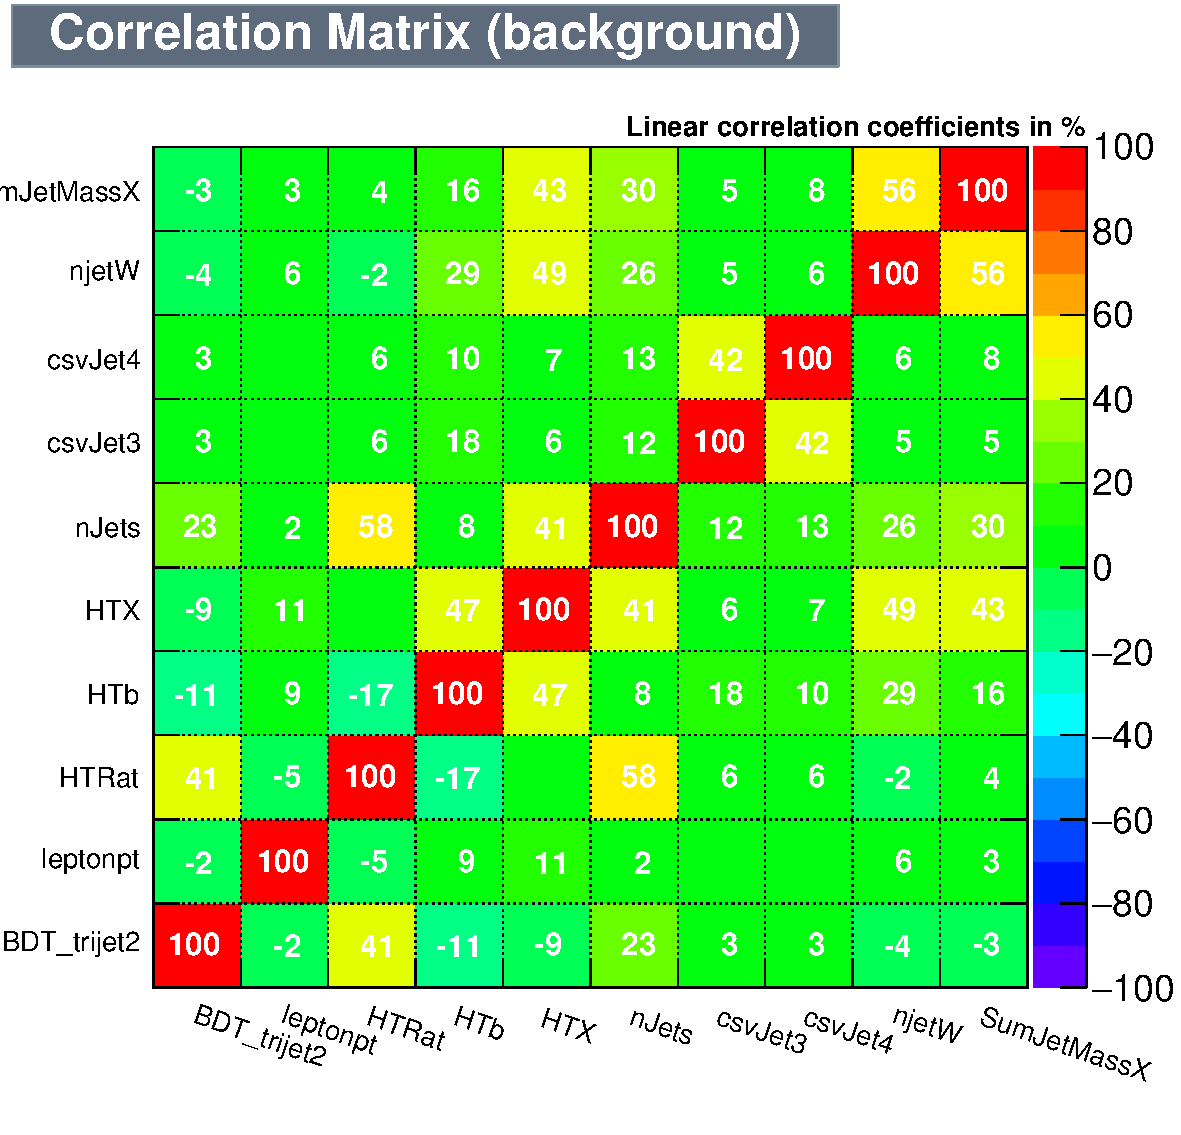
\includegraphics[width=0.48\textwidth]{images/Run2/CorrelationMatrixB.pdf}
    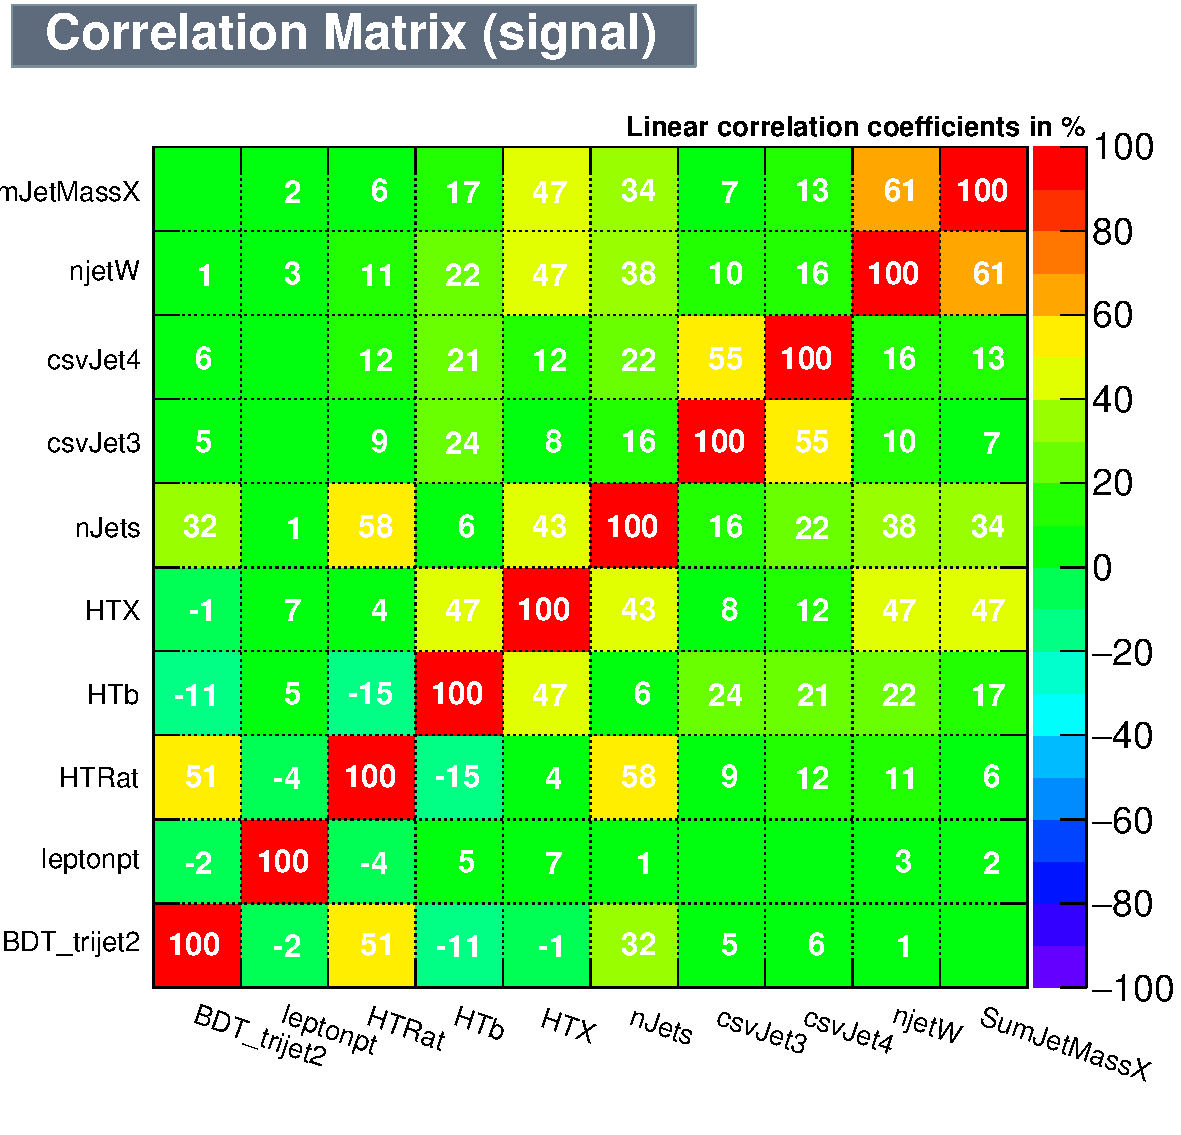
\includegraphics[width=0.48\textwidth]{images/Run2/CorrelationMatrixS.pdf}
    \caption{The correlation matrices for background (left) and signal (right).}
    \label{fig:corrMat}
\end{figure}

Correlation matrices were used when choosing which variables to include in the final set which was used to train the BDT for this analysis. Highly correlated variables were removed as they are largely superfluous.

\subsubsection{Overtraining tests}

Figure~\ref{fig:ROC} shows the BDT distribution from training and testing (left) and the associated ROC curve for this training. The training sample is shown as a filled histogram and the testing sample is shown as overlaid data points for the signal \tttt (blue) and background \ttbar for red. It can be seen that there is good agreement between the training and testing samples with Kolmogorov-Smirnov values of 0.159 for background and 0.998 for signal. This suggest that the BDT has not been overtrained.

\begin{figure}
    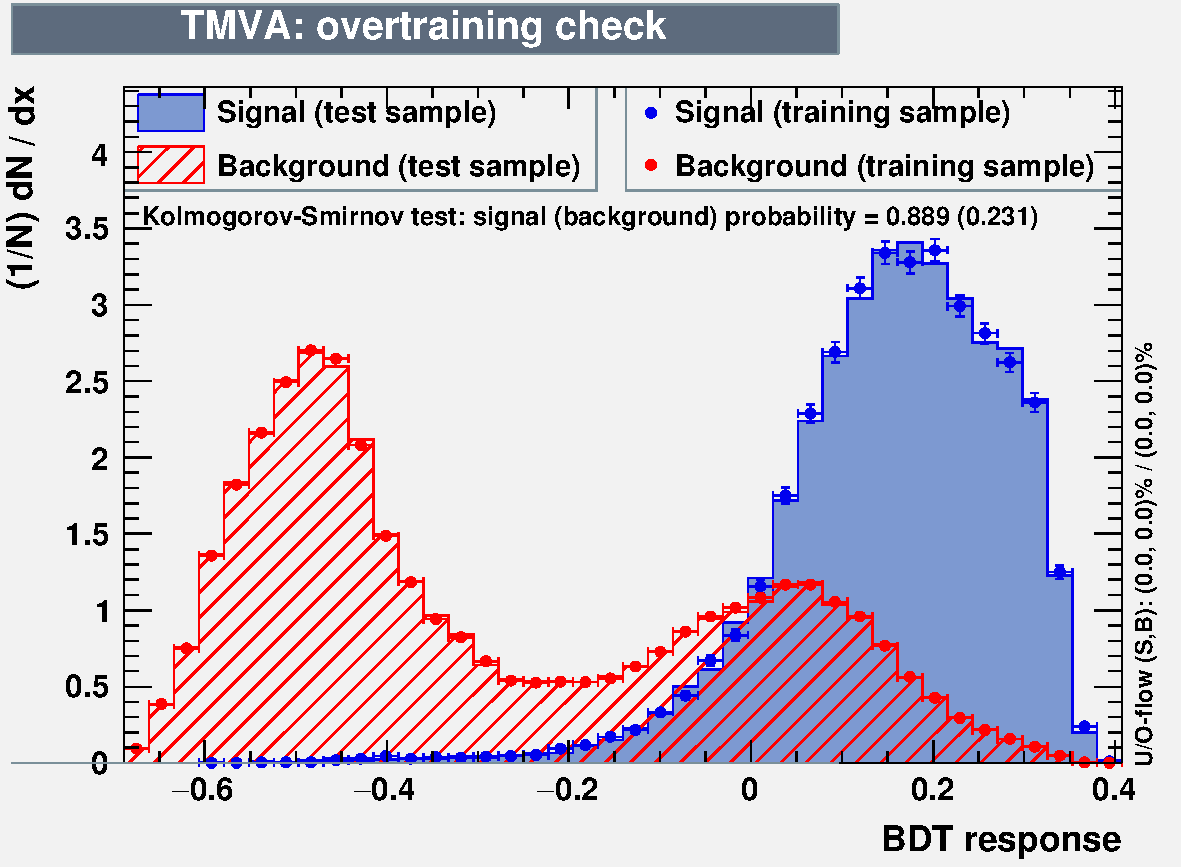
\includegraphics[width=0.48\textwidth]{images/Run2/overtrain_BDT.pdf}
    \includegraphics[width=0.48\textwidth]{images/Run2/rejBvsS.pdf}
    \caption{The over-training test for the BDT (left) and the rejection of background \ttbar (red) vs signal \tttt (blue) (right).}
    \label{fig:ROC}
\end{figure}


\section{Systematic uncertainties}
\label{sec:uncertainties13}
All systematic uncertainties are described in Section~\ref{sec:uncertainties} and some further details about them are given below. The systematic shape templates can be found in Appendix~\ref{app:sysshapes}.

\begin{itemize}
\item \textbf{Luminosity}\\
The CMS Luminosity Group gave a recommendation of 2.7$\%$ uncertainty on the luminosity~\cite{CMS-PAS-LUM-15-001} which is applied to all simulated backgrounds.
\item \textbf{Monte Carlo cross sections}\\
The uncertainty on the main background of \ttbar is ${}^{+2.5\%}_{-3.4\%}$ renormalisation and factorisation scale and ${}^{+6.2\%}_{-6.4\%} \left( \textrm{PDF} \right)$~\cite{PhysRevLett.110.252004}. The MC cross section uncertainties for the other background processes are modelled by assigning a $4\%$ uncertainty and a $10\%$ uncertainty is assigned to the signal process.
\item \textbf{Lepton SF}\\
The lepton SF is applied to all backgrounds. The uncertainty on these SFs is 1.3$\%$ in muon channel and 3.6$\%$ in electron channel
\item \textbf{Matrix Element Factorisation and renormalisation scales}\\
Weights are available in the \ttbar and \tttt samples which correspond to the factorisation and renormalisation scale $\left(\mu_{f},~\mu_{s}\right)$ being individually varied through 1/2u, u and 2u, where u represents the central value. This gives nine weights however the extreme unphysical values of (1/2u, 1/2u) and (2u, 2u) are not included. Applying these weights individually gives six alternative event-level BDT histograms to the central histogram, which uses (u,u). 
\item \textbf{Parton Shower Factorisation and renormalisation scales}\\
The effect of the parton showering (PS) scale in the \PYTHIA~8 generator is evaluated by using alternative \ttbar samples with the PS scale (u$_{PS}$) varied by 2u$_{PS}$, 1/2u$_{PS}$. This shift in the PS scale is equivalent to modifying the value of $\alpha_{S}$ hence the alternative parton shower histogram shapes have been inflated by a factor of 1.5 relative to the nominal template to take into account the uncertainty on the jet multiplicity modelling.
\item \textbf{\ttbar generator}\\
The \POWHEG generator was used to produce the nominal \ttbar sample for this analysis. The dependence of the generator can be estimated by running the analysis with the \MLM and \MADGRAPH\aMCATNLO~FxFx \ttbar samples. A symmetric envelope is formed around the nominal by symmetrising the difference in event counts in each bin between the alternative and nominal samples. The \MLM sample was found to produce the most conservative uncertainty for this effect and so it was used to produce the symmetric up and down histograms.
\item \textbf{JES}\\
The JES uncertainty is derived by varying the JES by $\pm1\sigma$ for the \ttbar and \tttt samples.
\item \textbf{JER}\\
The JER uncertainty is derived by varying the smearing by $\pm1\sigma$ for the \ttbar and \tttt samples.
\item \textbf{b tagging}\\
As detailed in Section~\ref{sec:Calibrations13}, the difference between b-tagging efficiency in data and simulation is accounted for by the application of scale factors to simulated events via an event weighting procedure. This is the event weighting procedure was developed for Ref.~\cite{CMS-PAS-HIG-16-004}, details of which are documented here~\cite{CMS-NOTE-2013-130}. Given the significant uncertainty on these scale factors and that the CSV distributions are input variables to the BDT algorithm, a significant systematic effect is expected. Light flavour contamination, `lf', and linear statistical and quadratic statistical fluctuations, `hfstats1' and `hfstats2', are applied to heavy flavour jets. Heavy flavour contamination, `hf', and linear statistical and quadratic statistical fluctuations, `lfstats1' and `lfstats2', are applied to light flavour jets. Linear and quadratic uncertainties, `cferr1' and `cferr2', are applied to charm flavour jets. A b-tagging JES systematic is applied to light and heavy flavour jets when the standard jet energy scale systematics are applied and hence it is incorporated into the alternative JES systematic shapes. The b-tagging systematic is studied for the \ttbar and \tttt samples.
\item \textbf{Pile up}\\
The PU systematic uncertainty is found by varying the MinBias cross section by $\pm5\%$ and is applied to the \ttbar and \tttt samples.
\item \textbf{\heavyflavourone / \heavyflavourtwo modelling}
The uncertainty on the measurement of \heavyflavourone / \heavyflavourtwo by CMS~\cite{Khachatryan2015132} is $\pm 0.3 \left( \textrm{stat.} \right) \pm 0.6 \left(\textrm{sys.} \right)$. Alternative event weights are derived for \heavyflavourone / \heavyflavourtwo which are used to provide the alternative systematic up and down histograms.
\end{itemize}



\section{Template fit and upper limit}
\label{sec:limit13}
As no excess of events over the background expectation consistent with SM $\tttt$ production was observed, upper limits on $\sigma_{\tttt}^{SM}$ are calculated. 
The limit setting proceeds by simultaneously fitting the BDT output distributions of signal and backgrounds to the BDT distribution of data in both the $\mu$ + jets and $e$ + jets channels in all 12 \njets and \nMtags categories. The Higgs Combine Tool is used to perform the fit, assigning lognormal uncertainties to normalisation systematic uncertainties and the vertical morphing technique described in Section~\ref{sec:limitFit} for the shape systematic uncertainties. The fit produces a fitted shape and normalisation and best-fit values for all nuisance parameters and the parameter of interest. 
To avoid prohibitively large computing times, the approximate \emph{asymptotic} approach is used to calculate the \CLS limits, which can be found in Table~\ref{tab:limits} in units of $\sigma_{SM}$. 

\begin{table}[ht!]
\centering
\begin{tabular}{| l | c | c | c | c | c |}
  \hline
Channel  & Expected limit & Uncertainty & Observed limit\\
 \hline
$\mu$  &$20.6$ & $+12.9 -7.2$ & $20.8$ \\
 \hline
e  &  $26.4$ & $+16.6 -9.3$ & $33.5$ \\
 \hline
 Combined  &  $16.0$ & $+9.8 -5.5$ & $16.8$ \\
 \hline
\end{tabular}
 \caption{Extracted expected limits for \njets and \nMtags categorized templates in multiples of $\sigma_{SM}$.}
  \label{tab:limits}
  \end{table}

The combined expected limit is $147.2^{+90}_{-51}$~fb and the observed limit is 154.6~fb for the single lepton + jets channel.

\subsubsection{Nuisance parameters}

Figure~\ref{fig:datanuis} shows the variation of the post-fit nuisance parameters, $\theta$, with respect to their pre-fit values. As all of the parameters have not shifted outside of the pre-fit uncertainty, the number of uncertainties and their modelling is deduced to be appropriate for modelling the data. It can be seen that both the \ttbar ME scale uncertainty and the PS scale, denoted \emph{ttMEScale} and \emph{scaleH} respectively on the plot, have much smaller post-fit uncertainties with respect to their pre-fit uncertainties which suggests that they were larger than necessary.

\begin{figure}[h!]
\begin{center}
\subfloat{
\includegraphics[width=0.92\textwidth]{images/Run2/Nuisances.pdf}}
\hspace{0.2cm}
\end{center}
\caption{Post-fit nuisance parameters for data.}
\label{fig:datanuis}
\end{figure} 

% \section{Systematics studies and tests on analysis}

% \subsection{Ranking of variables in BDT}

% \begin{table}[ht!]
% \centering
% \begin{tabular}{| l | l | l | p{5cm} |}
%   \hline
% Rank & Variable & Importance \\
%  \hline
% 1 & \njets & 1.340e-01\\
% 2 & third highest CSV &1.180e-01\\
% 3 & \htrat & 1.133e-01\\
% 4 & BDT$_{trijet2}$ & 1.091e-01 \\
% 5 & \njetsw &1.082e-01\\
% 6 & \redhadmass& 1.026e-01\\
% 7 & HTX & 9.867e-02\\
% 8 & \htb & 8.650e-02 \\
% 9 & fourth highest CSV & 7.630e-02\\
% 10 & leadleppt & 5.334e-02  \\

% \hline
% \end{tabular}
%  \caption{Ranking of variables in order of discrimination power within the BDT.}
%   \label{tab:BDTrankings}
%   \end{table}



% \subsection{Correlation matrices for fit nuisance parameters}


% The correlation matrix for the fit nuisance parameters in the background only scenario can be see in Fig.~\ref{fig:FitCorr}. There is some correlation between the various b-tagging scale factors and also a correlation between the heavy flavour \heavyflavourone / \heavyflavourtwo modelling and the \ttbar ME scale, where the \heavyflavourone / \heavyflavourtwo is expected to be related to the choice of ME scale.

% \begin{figure}[ht!]
%     \includegraphics[width=0.9\textwidth]{images/Run2/FitCorr.pdf}
%     \caption{The correlation matrices for background only for the fit parameters.}
%     \label{fig:FitCorr}
% \end{figure}




% \subsection{Studies of impact of systematic uncertainties}

% The impact of each systematic uncertainty on the expected limit is shown in Table~\ref{tab:sysRemoved} by removing each systematic from the fit and recalculating the expected limit. The systematic uncertainties which have the largest impact are the \ttbar ME scale, \ttbar PS scale and the JES scale, which is applied to both \ttbar and \tttt. The \ttbar ME scale has a large impact on the modelling of the signal process whereas the \ttbar PS scale has a big effect on the modelling of the additional jets produced in high jet multiplicity \ttbar events which pass the baseline event selection.

% \begin{table}[ht]
% \centering
% \caption{Expected limits on \tttt production which each systematic removed in turn}
% \label{tab:sysRemoved}
% \begin{tabular}{|l|l|}
% \hline
% % \rule{0pt}{4ex}    
% % \rule[-1.2ex]{0pt}{0pt}
% Systematic uncertainty removed & Expected limit ($\times$\sigmattttsm) \T \B\\ 
% % \rule{0pt}{4ex}    

% \hline
% None                           & 16.0000                                                         \\ \hline
% \ttbar ME scale                & 16.0625                                                         \\ \hline
% \tttt ME scale                 & 14.4375                                                         \\ \hline
% JER                            & 15.9375                                                         \\ \hline
% JES                            & 15.3125                                                         \\ \hline
% PS scale                       & 15.0625                                                         \\ \hline
% PU                             & 16.0625                                                         \\ \hline
% Generator uncertainty          & 15.9531                                                         \\ \hline
% \ttbar heavy flav              & 15.5625                                                         \\ \hline
% Luminosity                     & 16.0625                                                         \\ \hline
% Lepton SF Mu                   & 16.0625                                                         \\ \hline
% Lepton SF El                   & 15.9062                                                         \\ \hline
% \ttbar norm                    & 16.0000                                                         \\ \hline
% \tttt norm                     & 15.9062                                                         \\ \hline
% EW norm                        & 16.0000                                                         \\ \hline
% Single top norm                & 16.0000                                                         \\ \hline
% % b-tag light SF                 & 12.5625                                                         \\ \hline
% btagWeightCSVCFErr1            & 16.0625                                                         \\ \hline
% btagWeightCSVCFErr2            & 16.0625                                                         \\ \hline
% btagWeightCSVHF                & 15.5625                                                         \\ \hline
% btagWeightCSVHFStats1          & 15.9375                                                         \\ \hline
% btagWeightCSVHFStats2          & 15.9531                                                         \\ \hline
% btagWeightCSVLF                & 15.9375                                                         \\ \hline
% btagWeightCSVLFStats1          & 16.0625                                                         \\ \hline
% btagWeightCSVLFStats2          & 15.9062                                                         \\ \hline
% \end{tabular}
% \end{table}

% The impact of each systematic uncertainty on the expected and observed limit is shown in Table~\ref{tab:sysRemoved} but removing each systematic from the fit.

% \begin{table}[ht]
% \centering
% \caption{Limits on \tttt production which each systematic removed in turn}
% \label{tab:sysRemoved}
% \begin{tabular}{|l|l|l|}
% \hline
% Systematic uncertainty removed & Expected limit ($\times$\sigmattttsm) & Observed limit ($\times$\sigmattttsm) \\ \hline
% None                           & 16.0000                             & 16.8340                             \\ \hline
% \ttbar ME scale                & 16.0625                             & 16.4804                             \\ \hline
% \tttt ME scale                 & 14.4375                             & 15.3639                             \\ \hline
% JER                            & 15.9375                             & 16.9774                             \\ \hline
% JES                            & 15.3125                             & 17.1332                             \\ \hline
% PS scale                       & 15.0625                             & 15.7623                             \\ \hline
% PU                             & 16.0625                             & 16.8574                             \\ \hline
% Generator uncertainty          & 15.9531                             & 16.6530                             \\ \hline
% \ttbar heavy flav              & 15.5625                             & 16.7846                             \\ \hline
% Luminosity                     & 16.0625                             & 16.7553                             \\ \hline
% Lepton SF Mu                   & 16.0625                             & 16.7646                             \\ \hline
% Lepton SF El                   & 15.9062                             & 16.1287                             \\ \hline
% \ttbar norm                    & 16.0000                             & 16.7771                             \\ \hline
% \tttt norm                     & 15.9062                             & 16.7785                             \\ \hline
% EW norm                        & 16.0000                             & 16.8358                             \\ \hline
% Single top norm                & 16.0000                             & 16.8370                             \\ \hline
% b-tag light SF                 & 12.5625                             & 15.8688                             \\ \hline
% btagWeightCSVCFErr1            & 16.0625                             & 16.1875                             \\ \hline
% btagWeightCSVCFErr2            & 16.0625                             & 16.8263                             \\ \hline
% btagWeightCSVHF                & 15.5625                             & 15.5625                             \\ \hline
% btagWeightCSVHFStats1          & 15.9375                             & 16.7888                             \\ \hline
% btagWeightCSVHFStats2          & 15.9531                             & 16.6833                             \\ \hline
% btagWeightCSVLF                & 15.9375                             & 16.7457                             \\ \hline
% btagWeightCSVLFStats1          & 16.0625                             & 16.8998                             \\ \hline
% btagWeightCSVLFStats2          & 15.9062                             & 16.7752                             \\ \hline
% \end{tabular}
% \end{table}

\section{Alternative limit setting using \texorpdfstring{\HT}~~ distributions for template fitting}

The limit setting procedure was repeated using the \HT distributions to perform the template fit. This is to compare a simple discriminating variable between \ttbar and \tttt to the output BDT discriminator variable to estimate the gain of using a BDT. 

\begin{table}[ht!]
\centering
\begin{tabular}{| l | c | c | c | c | c |}
  \hline
Channel  & Categorized & Uncertainty \T \B \\
 \hline
$\mu$  &$26.4$ & $+16.2 -9.2$  \\
 \hline
e  &  $30.6$ & $+18.8 -10.7$  \\
 \hline
 Combined  &  $19.6$ & $+11.7 -6.7$ \\
 \hline
\end{tabular}
 \caption{Extracted expected limits for \njets and \nMtags categorized templates of \HT in multiples of $\sigma_{SM}$.}
  \label{tab:HTlimits}
  \end{table}

The results in Table~\ref{tab:HTlimits} correspond to a combined expected limit of $180.3^{+108}_{-62}$ fb using \HT to make the template fit compared to an expected limit of $147.2^{+90}_{-51}$ fb when using the event level BDT to make the template fit. Hence, using the BDT the expected limit is improved by $\approx20\%$.

Further studies of the expected limit with each systematic removed can be found in Appendix~\ref{app:sysminusone}. The correlation matrix for the fit nuisance parameters can be found in Appendix~\ref{app:corrFit}.



\section{Combination with OS dilepton channel and SS dilepton channel ~\label{sec:combo13}}

The sensitivity of the search for standard model four top quark production can be improved by combining with other search channels. An opposite-sign (OS) search was developed in parallel with the single lepton channel study described in this chapter~\cite{CMS-PAS-TOP-16-016}. The analysis selects events which contain any combination of $\mu^{+}\mu^{-}$, $\mu^{\pm} e^{\mp}$, $e^{+}e^{-}$. It uses the same hadronic top quark reconstruction as in Section~\ref{sec:topContent13} to identify the BDT value for highest-ranked top quark candidate, $BDT_{trijet1}$. This variable is fed into the event-level BDT along with other variables based on the event-topology, event activity and b-jet content. A simultaneous fit was made using the BDT histogram templates described above for the single lepton channel and the BDT histogram templates (which are split only in \njets categories due to statistical limitations) from the dilepton channel. All systematic uncertainties apart from the lepton scale factors were treated as correlated. The results of this fit can be found in Table~\ref{tab:limits_combined} in the row labelled \emph{Combined (single lepton and OS dilepton)}. It is clear that the OS dilepton channel alone is not as sensitive as the single lepton channel, which is due in part to it having a smaller branching ratio, however its combination with the single lepton channel improves the overall sensitivity.\\

The analysis was then further combined with a search for new physics in events with same-sign (SS) dileptons which places limits on the SM production of four top quarks~\cite{Khachatryan:2016kod}. This search benefits from very low numbers of events from background processes which gives rise to its good signal sensitivity. The luminosity, JES and PU systematic uncertainties were treated as correlated between the SS dilepton channel and the other two channels. The uncertainty in response of the CMS trigger system to events containing dileptons is also treated as correlated between the two dilepton analyses, whilst all other systematic uncertainties were treated as fully uncorrelated between the SS dilepton analysis and the other two search channels. The combination of all channels is listed in Table~\ref{tab:limits_combined} where it can be seen that this gives a significant improvement in the expected limit compared to any individual channel.

\clearpage

\begin{table}[ht!]
%NOTE: THE VALUES ARE DEFINED IN THE TOP-16-016.tex at the start - modify them there, not here.
    \caption{Expected and observed 95\% CL upper limits on the SM \tttt production as a multiple of \sigmattttSM and in fb. The values quoted on the expected limits are the $1$ standard deviation uncertainties and include all statistical and systematic uncertainties.}    
    \centering
    \footnotesize
    \begin{tabular}{ l | c  |  c | c  | c }
        Channel  & Expected Limit  & Observed Limit & Expected limit  & Observed Limit \T \B\\  
         & (x \sigmattttSM) & (x \sigmattttSM) & (fb) & (fb) \T \Bbig \\ \hline \hline
                Single lepton  & $\xsecmusingleptonexp^{\,+\,\xsecmusingleptonup}_{\,-\,\xsecmusingleptondown}$ & $\xsecmusinglepton$ & $\xsecfbsingleptonexp^{\,+\,\xsecfbsingleptonup}_{\,-\,\xsecfbsingleptondown}$ & $\xsecfbsinglepton$   \T \B  \\ 
                  & & & &  \\ \hline

                Dilepton  & $\xsecmudileptonexp^{\,+\,\xsecmudileptonup}_{\,-\,\xsecmudileptondown}$ & $\xsecmudilepton$ & $\xsecfbdileptonexp^{\,+\,\xsecfbdileptonup}_{\,-\,\xsecfbdileptondown}$ & $\xsecfbdilepton$ \T \B   \\ 
                (opposite sign) & & & &  \\
            \hline 
                 Combined (single lep & $\xsecmucomboexp^{\,+\,\xsecmucomboup}_{\,-\,\xsecmucombodown}$ & $\xsecmucombo$  & $\xsecfbcomboexp^{\,+\,\xsecfbcomboup}_{\,-\,\xsecfbcombodown}$ & $\xsecfbcombo$   \T \B  \\
                -ton and OS dilepton) & & & &  \\   \hline            
                Dilepton & $11.0^{\,+\,6.2}_{\,-\,3.8}$ & $12.9$ & $101^{\,+\,57}_{\,-\,35}$ & $119$   \T \B  \\
                (same sign) & & &  & \\ \hline
                Combined  & $\xsecmucomboallexp^{\,+\,\xsecmucomboallup}_{\,-\,\xsecmucomboalldown}$ & $\xsecmucomboall$  & $\xsecfbcomboallexp^{\,+\,\xsecfbcomboallup}_{\,-\,\xsecfbcomboalldown}$ & $\xsecfbcomboall$  \T \B   \\
                (all channels) & & & &  \\                
    \end{tabular}
    \label{tab:limits_combined}
\end{table}

\section{Summary and conclusion}
\label{sec:summary13}

The SM production of four top quarks at $\sqrt{s} =$~13~TeV has been studied with 2.6~\fbinv of data from the 2015 CMS dataset. In the absence of an excess, limits were placed on the SM cross section, which is 9.2~fb. The single lepton channel was primarily studied in the $\mu$ + jets and e + jets final states. Baseline selection requirements were implemented to suppress backgrounds and select the signal \tttt process. Good agreement was observed between the simulation and data in many variables after corrections were applied to the events. BDTs were employed to reconstruct hadronically decaying top quarks and then to increase the separation of the signal and background processes using several discriminating variables including those formed from the hadronic top quark BDT. Many tests were performed to check the performance of the BDTs, that it didn't suffer from overtraining and was stable with respect to changing hyperparameters. Categorisation of the histograms going into the template fit was optimised to enhance the sensitivity of the analysis and hence reduce the expected limit. The limit set on the SM production of four top quarks is $16.0^{+9.8}_{-5.5}\times \sigmattttSM$ expected and $16.8\times \sigmattttSM$ observed which equates to $147.2^{+90}_{-51}$ expected and 154.6 fb observed.

\section{Discussion of other searches for \tttt production studies at $\sqrt{s} =$~13~TeV}
\label{sec:ATLASresult13}

There are a number of searches for the production of four top quarks at $\sqrt{s}=13$~TeV in the single lepton, opposite-sign dilepton and same-sign dilepton channels, and at both the CMS and ATLAS experiments. A summary of the results is given in Table~\ref{tab:CmsAtlasSum} including three CMS analyses in three different channels using the 2015 CMS dataset and a combination of those results as discussed in Section~\ref{sec:combo13}. The table also includes two different ATLAS searches, ATLAS-CONF-2016-013 and ATLAS-CONF-2016-020, which place limits on four-top-quark production in the single lepton channel using the 2015 ATLAS dataset of 3.2~\fbinv. ATLAS-CONF-2016-104 is a progression from ATLAS-CONF-2016-013 that uses the 2015 and 2016 ATLAS datasets using a total of 13.2~\fbinv. Finally there is a same-sign dilepton search by ATLAS which uses the 2015 ATLAS dataset with 3.2~\fbinv also.

Of all the analyses the same-sign dilepton searches are the most sensitive. 
ATLAS-CONF-2016-020 is more sensitive than ATLAS-CONF-2016-013 as it categorises into more jet and b-tag categories. There is a significant reduction in the limit between ATLAS-CONF-2016-013 and ATLAS-CONF-2016-140 of $\approx 40\%$ by using four times more data. The results, between searches in the same channels in CMS and ATLAS are compatible with each other within the systematic errors. Overall the CMS combination has the strongest limit on four-top-quark production so far of 66~fb (69$^{+37}_{-23}$~fb) observed (expected).

\begin{table}[h!]
\centering
\begin{tabular}{l|l|l|l|l}
% \hline
\multicolumn{1}{c|}{Analysis} & \multicolumn{1}{c|}{Channel} & \multicolumn{1}{c|}{$\mathcal{L}$ (\fbinv)} & \multicolumn{1}{c|}{Expected}  & \multicolumn{1}{c}{Observed } \\ 
 & & & \multicolumn{1}{c|}{limit (fb)} & \multicolumn{1}{c}{limit (fb)} \B \\ \hline \hline 
CMS (This analysis)                 & Single lepton                & 2.6                                         & 147$^{+90}_{-51}$                                     & 155                                      \T \B \\ \hline
CMS                            & OS dilepton                  & 2.6                                         & 221$^{+150}_{-82}$                                      & 130                                      \T \B \\ \hline
CMS~\cite{Khachatryan:2016kod}                            & SS dilepton                  & 2.6                                         & 101$^{+57}_{-35}$                                      & 119                                      \T \B \\ \hline
CMS combination                & Above combined               & 2.6                                         & 69$^{+37}_{-23}$                                       & 66                                       \T \B \\ \hline
ATLAS-CONF-2016-013~\cite{ATLAS-CONF-2016-013}            & Single lepton                & 3.2                                         & 180                                      & 370                                      \T \B \\ \hline
ATLAS-CONF-2016-020~\cite{ATLAS-CONF-2016-020}            & Single lepton                & 3.2                                         & 143                                      & 190                                      \T \B \\ \hline
ATLAS-CONF-2016-032~\cite{ATLAS-CONF-2016-032}            & SS dilepton                  & 3.2                                         & 107                                      & 95                                       \T \B \\ \hline
ATLAS-CONF-2016-104~\cite{ATLAS-CONF-2016-104}            & Single lepton                & 13.2                                        & 110                                      & 130                                      \T \B \\ 
% \hline
\end{tabular}
\caption{Limits of four-top-quark production by a variety of searches in CMS and ATLAS at $\sqrt{s}=13$~TeV}
\label{tab:CmsAtlasSum}
\end{table}



